\documentclass[final]{fhnwreport}       %[mode] = draft or final
                                        %{class} = fhnwreport, article, 
                                        %          report, book, beamer, standalone
%%---Main Packages-----------------------------------------------------------------------
\usepackage[english, ngerman]{babel}	%Mul­tilin­gual sup­port for LaTeX
\usepackage[T1]{fontenc}				%Stan­dard pack­age for se­lect­ing font en­cod­ings
\usepackage[utf8]{inputenc}				%Ac­cept dif­fer­ent in­put en­cod­ings
\usepackage{lmodern}                    %The newer Font-Set
\usepackage{textcomp}					%LaTeX sup­port for the Text Com­pan­ion fonts
\usepackage{graphicx} 					%En­hanced sup­port for graph­ics
\usepackage{float}						%Im­proved in­ter­face for float­ing ob­jects
\usepackage{ifdraft}                    %Let you check if the doc is in draft mode

%%---Useful Packages---------------------------------------------------------------------
\usepackage[pdftex,dvipsnames]{xcolor}  %Driver-in­de­pen­dent color ex­ten­sions for LaTeX
\usepackage{csquotes}                   %Simpler quoting with \enquote{}
\usepackage{siunitx} 					%A com­pre­hen­sive (SI) units pack­age
\usepackage{listings}					%Type­set source code list­ings us­ing LaTeX
\usepackage[bottom]{footmisc}			%A range of foot­note op­tions
\usepackage{footnote}					%Im­prove on LaTeX's foot­note han­dling
\usepackage{verbatim}					%Reim­ple­men­ta­tion of and ex­ten­sions to LaTeX ver­ba­tim
\usepackage[textsize=footnotesize]{todonotes} %Mark­ing things to do in a LaTeX doc­u­ment

%%---Tikz Packages-----------------------------------------------------------------------
\usepackage{standalone}
\usepackage{tikz}
\usepackage{circuitikz}
\usetikzlibrary{arrows}
\usetikzlibrary{calc}
\usetikzlibrary{intersections}

%%---Math Packages-----------------------------------------------------------------------
\usepackage{amsmath}					%AMS math­e­mat­i­cal fa­cil­i­ties for LaTeX
%\usepackage{amssymb}					%Type­set­ting symbols (AMS style)
%\usepackage{array}						%Ex­tend­ing the ar­ray and tab­u­lar en­vi­ron­ments
%\usepackage{amsthm}					%Type­set­ting the­o­rems (AMS style)

%%---Table Packages----------------------------------------------------------------------
\usepackage{tabularx}					%Tab­u­lars with ad­justable-width columns
%\usepackage{longtable}
\usepackage{multirow}					%Create tab­u­lar cells span­ning mul­ti­ple rows
\usepackage{multicol}					%In­ter­mix sin­gle and mul­ti­ple columns

%%---PDF / Figure Packages---------------------------------------------------------------
\usepackage{pdfpages}					%In­clude PDF doc­u­ments in LaTeX
\usepackage{pdflscape}					%Make land­scape pages dis­play as land­scape
\usepackage{subfig}					    %Fig­ures di­vided into sub­fig­ures

%%---Other Packages----------------------------------------------------------------------
%\usepackage{xargs}                     %De­fine com­mands with many op­tional ar­gu­ments

%%---Bibliography------------------------------------------------------------------------
\usepackage[style=ieee,urldate=comp,backend=biber]{biblatex}
\addbibresource{literature/bibliography.bib}

%%---Main Settings-----------------------------------------------------------------------
\graphicspath{{./graphics/}}			%Defines the graphicspath
%\geometry{twoside=false}				    %twoside=false disables the "bookstyle"
\setlength{\marginparwidth}{2cm}
\overfullrule=5em						%Creates a black rule if text goes over the margins => debugging


%%---User Definitions--------------------------------------------------------------------
%%Tabel-Definitions: (requires \usepackage{tabularx})
\newcolumntype{L}[1]{>{\raggedright\arraybackslash}p{#1}}    %column-width and alignment
\newcolumntype{C}[1]{>{\centering\arraybackslash}p{#1}}
\newcolumntype{R}[1]{>{\raggedleft\arraybackslash}p{#1}}

%%---Optional Package Settings-----------------------------------------------------------
%Listings-Settings: (requires \usepackage{listings}) => Example with Matlab Code
\lstset{language=Matlab,%
    basicstyle=\footnotesize\ttfamily,
    breaklines=false,%
    morekeywords={switch, case, otherwise},
    keywordstyle=\color{Blue},%
    tabsize=2,
    %morekeywords=[2]{1}, keywordstyle=[2]{\color{black}},
    identifierstyle=\color{Black},%
    stringstyle=\color{Purple},
    commentstyle=\color{Green},%
    showstringspaces=false,%without this there will be a symbol in the places where there is a space
    numbers=left,%
    numberstyle={\tiny \color{black}},% size of the numbers
    numbersep=9pt, % this defines how far the numbers are from the text
    %emph=[1]{word1, word2,...},emphstyle=[1]\color{red}
}										                %loads all packages, definitions and settings												
\title{Drahtlose Energie- und Datenübertragung}          %Project Title
\author{P5 Fachbericht}          		%Document Type => Technical Report, ...
\date{Windisch, {\today}}             	%Place and Date

\begin{document}

%%---TITLEPAGE---------------------------------------------------------------------------
\selectlanguage{ngerman}                %ngerman or english
\maketitle

\vspace*{-1cm}						    %compensates the space after the date line.
\vfill
\begin{figure}[H]
\centering
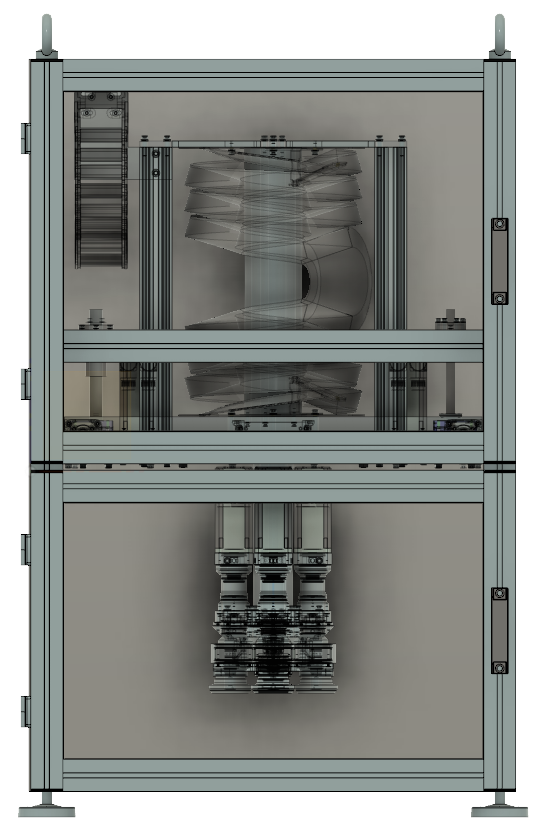
\includegraphics[width=0.4\linewidth]{mit_geruest}
\end{figure}
\vfill

{
\renewcommand\arraystretch{2}
\begin{center}
\begin{tabular}{>{\bf}p{4cm} l}
Hochschule                 &    Hochschule für Technik - FHNW\\
Studiengang                &    Elektro- und Informationstechnik\\
Autor   		           & 	Adrian Annaheim und Simon Zoller\\
Betreuer                   &    Schleuniger Pascal\\
Auftraggeber               &    Ferrum AG\\
Version                    &    1.0 %Normally not used!
\end{tabular}
\end{center}
}

\clearpage
			
%%---ABSTRACT----------------------------------------------------------------------------
%\selectlanguage{ngerman}				%ngerman or english
%\thispagestyle{empty}
%\begin{abstract}
Das Institut für Automation entwickelt einen neuen Dosenverschliesser in Zusammenarbeit mit der Ferrum AG. Weil eine Schleppkette zur Kabelführung für industrielle Maschinen weniger geeignet ist, soll diese ersetzt werden. Ziel dieser Arbeit ist es, ein Konzept zur berührungslosen Daten- und Energieübertragung zu entwickeln, welches die Schleppkette ablösen kann. Dafür ist eine Leistung von mindestens \SI{300}{W}/\SI{48}{V} und eine Geschwindigkeit von \SI{31.25}{MHz} notwendig. In dieser Arbeit werden durch Simulationen und Versuchsaufbauten wichtige Erkenntnisse für die spätere Umsetzung gesammelt. Die Energieübertragung wird durch ein induktives Verfahren realisiert. Die Datenübertragung findet über den optischen Weg statt.
\newline
Die Schaltungstopologie des Flybacks zur Energieübertragung eignet sich nicht für diese Anwendung, weil durch den geringen Kopplungsfaktor hohe Verluste verursacht werden. Die Testschaltung zur Datenübertragung kann ein Rechtecksignal mit \SI{45}{MHz} übertragen und übertrifft somit die geforderte Geschwindigkeit. Acrylglas eignet sich als lichtleitendes Material und kann somit als Kanal verwendet werden.
\\
\paragraph{Keywords:} Acrylglas, Ethernet, Flyback, induktive Energieübertragung, Infrarot, Kopplungsfaktor, optische Datenübertragung, Photodiode, Transimpedanzverstärker, VARAN-Bus, 
\end{abstract}



%%---TABLE OF CONTENTS-------------------------------------------------------------------
\pagenumbering{Roman}		
\selectlanguage{ngerman}				%ngerman or english
\tableofcontents
\clearpage

%%---TEXT--------------------------------------------------------------------------------
\pagenumbering{arabic}
\section{Einleitung}


\begin{figure}
\centering
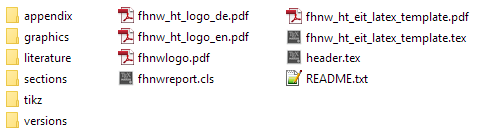
\includegraphics[width=0.8\linewidth]{ordner_struktur.png}
\caption{Minimalstruktur des \LaTeX -Projekts.}\label{fig:Struktur}
\end{figure}


\section{Grundlagen}\label{sec:Grundlagen}

-aktuelle Situation mit Bild (Maschine)
-Probleme dieser Lösung
-Konzept neu / alt Bild(Konzept)
-ev. Vorteil
Power-Kabel soll durch Induktive Übertagung und Daten-Bus soll durch optische Übertragung gelöst werden.


\subsection{Grundlagen zur Energieübertragung}
In diesem Unterkapitel werden die Grundlagen zur Energieübertragung erläutert. Das Kernstück der induktiven Übertragung ist ein Transformator. Dieser muss mit einer Schaltung angesteuert werden, damit sich das Magnetfeld ändert und Energie übertragen werden kann. Mittels dieser Grundlagen soll die Theorie des Transformators und der Schaltung vermittelt werden.

\paragraph{Transformator}
Ein Transformator besteht im wesentlichen aus zwei eng gekoppelten Wicklungen oder Induktivitäten die meistens auf einem gemeinsamen Kern aus Eisen liegen. 

Der Kopplungsfaktor gibt Aufschluss darüber, wie stark die gegenseitige magnetische Beeinflussung zweier oder mehreren benachbarten Drahtschleifen durch Induktion infolge einer magnetischen Flussänderung ist. Die Schleifen, wie in Abbildung \ref{eq:kopplungsfaktor}, nennt man ideal gekoppelt, weil der magnetische Fluss der einen Drahtschleife vollständig von der anderen umschlossen wird. \textcolor{red}{[Technische Elektrizitätslehre]}

\begin{figure}[H]
	\centering
	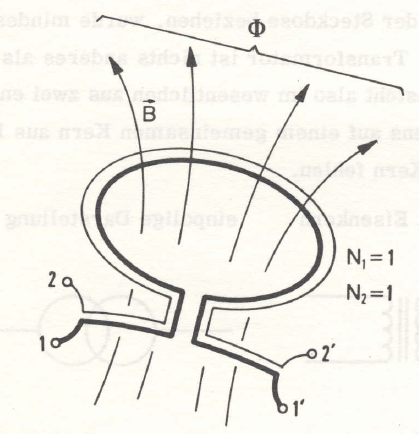
\includegraphics[width=0.4\linewidth]{kopplungsfaktor}
	\caption{Zwei ideal gekoppelte Einzelschleifen}\label{fig:kopplungsfaktor}
\end{figure}
Wenn sich in einer der beiden Schleifen der Strom ändert, induziert dieser sowohl in der eigenen als auch in der anderen Schleife dieselbe Spannung. Daher gilt Induktivität $ L_{1}$ = Induktivität $L_{2}$ = gesamte Gegeninduktivität $M$.
So lässt sich der Kopplungsfaktor $ k $ wie folgt definieren:
\begin{equation}
k=\frac{M}{\sqrt{L_{1}\cdot L_{2}}} = 1
\label{eq:kopplungsfaktor}
\end{equation}

In der Abbildung \ref{fig:trafo} ist ein ideal gekoppelter Transformator abgebildet. Die Ausgangsklemmen 2-2' sind offen was bedeutet, dass sich die Sekundärseite im Leerlauf befindet. 
\begin{figure}[H]
	\centering
	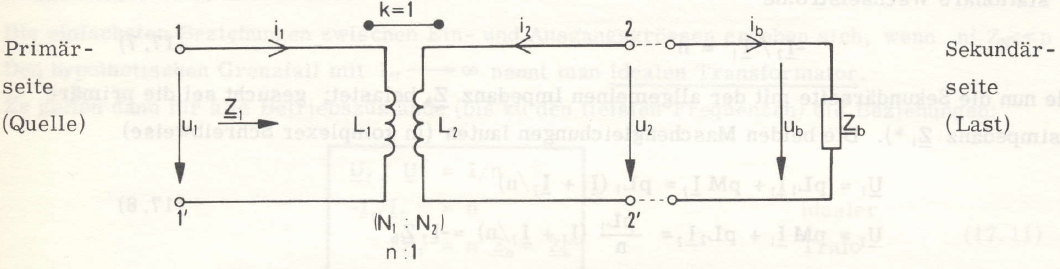
\includegraphics[width=1\linewidth]{grundlagen_trafo}
	\caption{Transformator mit ideal gekoppelten Spulen}\label{fig:trafo}
\end{figure}
In diesem Fall kann die Spannung $ u_{1} $ wie folgt berechnet werden.
\begin{equation}\label{eq:induktionsspannung}
u_{1}=L \cdot \frac{\mathrm{d} i_{L}}{\mathrm{d} t}
\end{equation}
Das Übersetzungsverhältnis ist beim idealen Transformator folgendermassen definiert.
\begin{equation}\label{eq:übertragung}
ü= \frac{N_{1}}{N_{2}} = \frac{U_{2}}{U_{1}}
\end{equation}

Lässt man nun die Voraussetzung der ideal gekopplten Spulen fallen, verhalten sich die induzierten Spannungen an zwei Induktivitäten nicht mehr wie die Windungszahlen. Die beiden Induktivitäten werden nun in einen ideal gekoppelten Teil und einen überhaupt nicht gekoppelten Teil aufgespaltenen. Der nicht gekoppelte Teil wird als Streuinduktivität bezeichnet. Sie hat Auswirkungen auf die Funktionsweise (Überspannung, Schwingungen nach Abschaltvorgängen) und Verluste von leistungselektronischen Schaltungen. Aus diesem Grund ist es wichtig einen möglichst idealen Kopplungsfaktor zu erreichen damit die Streuinduktivität klein ist. 
\newpage

\paragraph{Flyback-Converter}
Um eine Magnetfeldänderung zu erzeugen wird eine Schaltung benötigt. Die verwendete Schaltung wird Flyback-Converter oder auf Deutsch Eintakt-Sperrwandler genannt. Sie gehört zu den primär getakteten Wandlern. Die Eingangs- und Ausgangsseite sind galvanisch getrennt. Er wird in Schaltnetzteilen von kleiner bis mittleren Leistung (ca. 500W), z.B. für PC-Netzteilen, Drucker und Fernsehgeräte eingesetzt. \textcolor{red}{[Speerwandler, schulz]}
\\\\
Die Schaltung besteht aus wenigen Bauteile. Dies sind ein Schalter, ein Speichertransformator, eine Diode und ein Kondensator. Der Schalter, z.B. ein MOSFET, wird mit einem konstanten Tastgrad und Frequenz gesteuert. \textcolor{red}{[bachelor]}

\centering
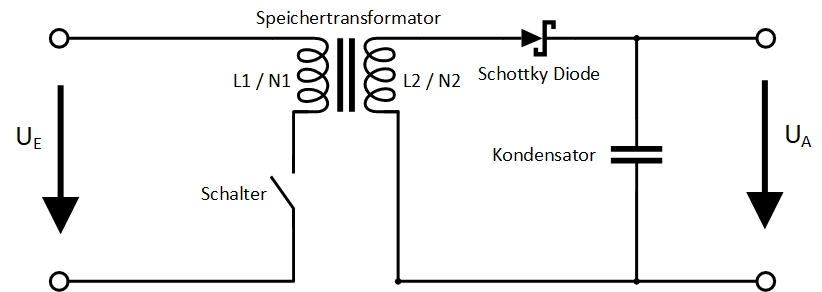
\includegraphics[width=1\linewidth]{flyback_schaltung}
\caption{Grundschaltung Flyback}\label{fig:flyback_schaltung}
\end{figure}

Wie man in Abbildung \ref{fig:flyback_schaltung} erkennen kann, beinhaltet die Schaltung einen Speichertransformator. Er dient zur dynamischen Energiespeicherung sowie für die Potenzialtrennung. Im Speichertransformator wird die gesamte übertragene Energie zwischen den einzelnen Zuständen im Magnetfeld zwischengespeichert. Aus diesem Grund benötigt er einen Luftspalt im Kern, da in diesem Teil die meiste magnetische Feldenergie gespeichert wird. Die beiden Wicklungen der Primär- und Sekundärseite müssen sehr gut magnetisch gekoppelt sein, damit die eingespeicherte Energie wieder abgegeben werden kann. Im Gegensatz dazu wird wegen der gleichzeitigen Leistungsaufnahme und -abgabe bei gewöhnlichen Transformatoren nur wenig Energie im Kern gespeichert.  \textcolor{red}{[schulz, speerwandler]}
Der Flyback überträgt basierend auf diesem Prinzip seine Energie erst auf die Sekundärseite, wenn der Schalter auf der Primärseite geöffnet wird. Der Flyback ist prinzipiell kurzschlussfest, da die Diode auf der Sekundärseite sperrt, sobald der Schalter geschlossen wird. Die genauere Funktionsweise ist in der Tabelle \ref{tab:funktionsweise} aufgeführt. \textcolor{red}{[schulz]}

	\centering
	\begin{tabular}{L{7cm}| L{7cm} }
		\multicolumn{1}{c|}{\textbf{Schalter geschlossen}}
		& \multicolumn{1}{c}{\textbf{Schalter geöffnet}} \\ \hline\hline
		$ \bullet $ Induktivität des Transformator lädt sich auf & $ \bullet $ Endmagnetisierung über die Sekundärwicklung \\ 
		$ \bullet $ Transformator ist im Leerlauf & $ \bullet $ Laden des Kondensators auf $ U_{A} $ \\ 
		$ \bullet $ Diode ist in Sperrrichtung &  \\ \hline
	\end{tabular}
	\caption{Funktionsweise des Flybacks \textcolor{red}{[schulz]}}\label{tab:funktionsweise}
\end{table}

	\centering
	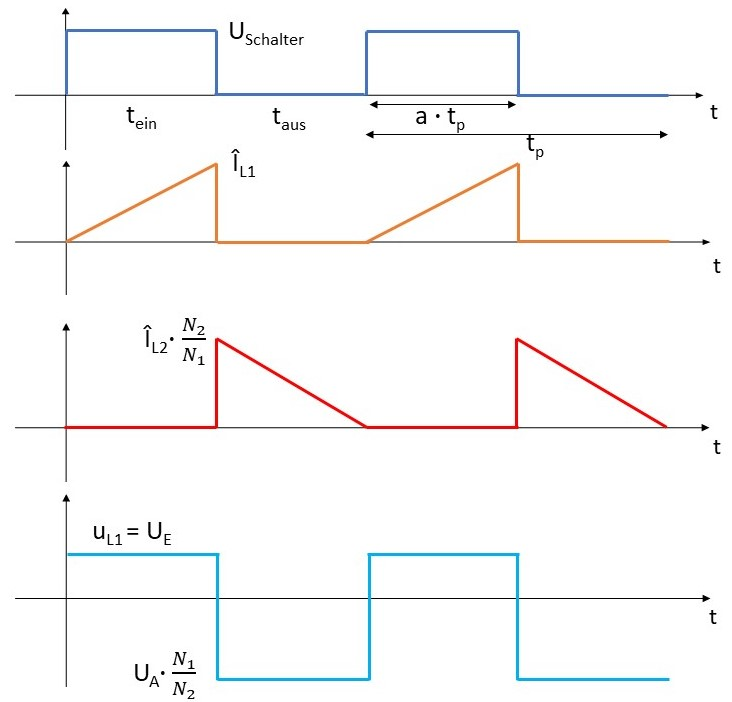
\includegraphics[width=0.9\linewidth]{kurven}
	\caption{Strom und Spannungsverlauf des Speichertrafos}\label{fig:kurven}
\end{figure}

Die Abbildung \ref{fig:kurven} zeigt, dass während der Leitphase des MOSFET die Primärspannung $ u_{L1} $ des Trafos gleich der Eingangsspannung $ U_{E} $ ist. In dieser Zeit steigt der Strom $ i_{L1} $ linear an. Die Primärspannung wird mit der Formel \ref{eq:induktionsspannung} beschrieben. Die Primäspannung $ u_{L1} $ lässt sich in diesem Fall mit der Eingangsspannung $ U_{E} $  und $ \mathrm{d} t $ mit $ a \cdot T_{p} $ darstellen. Nun kann die Formel wie folgt nach $ \^{I}_{L1} $ umgeformt werden.

\begin{equation}\label{eq:strom}
\^{I}_{L1}=\frac{U_{E}}{L}\cdot a \cdot T_{p}
\end{equation}

Um die nachfolgenden Formeln zu vereinfachen, wird das Übersetzungsverhältnis $ ü $ aus der Formel \ref{eq:übertragung} eingesetzt. Die Primärspannung $ u_{L1} $ muss im stationärem Betrieb einen Mittelwert gleich Null haben. Ansonsten würde der Strom auf unermesslich hohe Werte ansteigen. Das Tastverhältnis hat den Kennbuchstaben $ a $. Daraus folgt $ 0= U_{E} \cdot a + ü \cdot (-U_{A}) \cdot (1-a) $. Diese Gleichung lässt sich auch wie folgt schreiben:

\begin{equation}\label{eq:ausgangsspannung}
U_{A}= \frac{1}{ü} \cdot \frac{a}{1-a} \cdot U_{E}
\end{equation}

Die Energie, welche pro Periode übertragen wird, ist wie folgt zu berechnen:

\begin{equation}\label{eq:energie}
E= \frac{1}{2} \cdot L \cdot \^{I}_{p}\!^{2}
\end{equation}

Die übertragene Leistung hängt von der zwischengespeicherten Energie pro Periode und der Schaltfrequenz ab. Dies ergibt folgende Formel:

\begin{equation}\label{eq:Leistung}
P= f_{p} \cdot E = \frac{U_{2}\!^{2}}{R}
\end{equation}

\paragraph{Snubber}
Eine elektrische Schaltung, welche störende Spannungsspitzen neutralisieren soll, wird Snubber genannt. Solche Spannungsspitzen treten beim Schalten von induktiven Lasten auf, wenn der Strom abrupt unterbrochen wird. Dies ist auch beim Flyback der Fall, wenn der Schalter geöffnet wird. Aufgrund der Streuinduktivität des Speichertransformator steigt die Drain-Source-Spannung am MOSFET stark an. Diese Spannung kann den MOSFET beschädigen. Um diese Überspannung zu verhindern, gibt es verschiedene Möglichkeiten.

Ein Snubber zu dimensionieren, ist nicht ganz einfach den neben der Spannungsbegrenzung müssen noch weitere Probleme gelöste werden. Folgende Punkte müssen gelöst werden:
\begin{itemize}
	\item Spannungsbelastung des MOSFET auf ein aktzeptables Mass begrenzen
	\item Streuinduktivität möglichst zügig entladen, um den Wirkungsgrad hoch zu halten
	\item Schaltverluste dürfen nur minimal erhöht werden durch das Hinzufügen des Snubber-Glieds
	\item Auswirkungen auf das dynamische Verhalten des Netzteils zu vermeiden
\end{itemize}
Nachfolgend werden zwei Typologien vorgestellt.

	\centering
	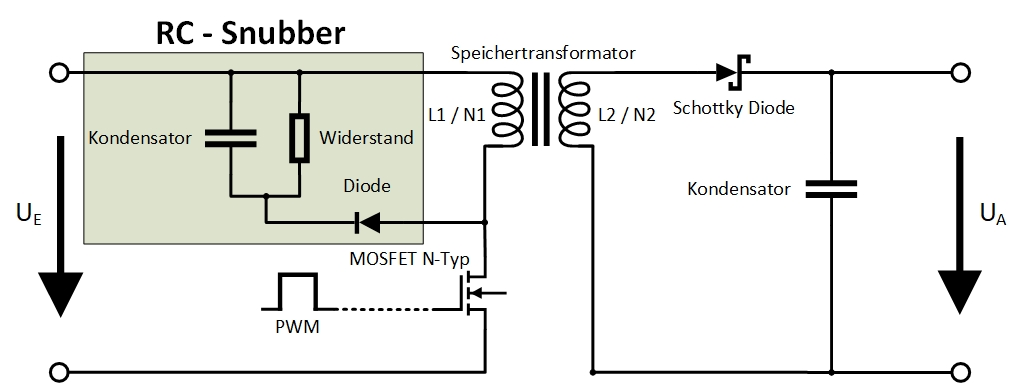
\includegraphics[width=0.9\linewidth]{Flyback_RC}
	\caption{Snubberschaltung mit RC-Glied}\label{fig:Flyback_RC}
\end{figure}

In der Abbildung \ref{fig:Flyback_RC} wird die Snubberschaltung mit einem Widerstand, einem Kondensator und einer Diode realisiert. Diese Schaltung basiert darauf, dass die überschüssige Energie aus der Streuinduktivität des Übertrags in den Snubber-Kondenstor geleitet wird. Die Differenz zwischen der Begrenzungs- und der Rest-Spannung ist gleich der Spannung über die Streuinduktivität. Die im Widerstand umgesetzte Verlustleistung und der Energiebetrag in der Streuinduktivität legen die Begrenzungsspannung dieser Schaltung fest. Ein kleiner Widerstand setzt die Begrenzungsspannung herab, jedoch entsteht eine höhere Verlustleistung. 

Der Nachteil dieser Schaltung ist, je weiter die Begrenzungsspannung gesenkt wird, desto mehr Energie wird der Gesamtleistung entzogen. Daher entsteht ein schlechterer Wirkungsgrad. \textcolor{red}{[power-tipps 17]}

	\centering
	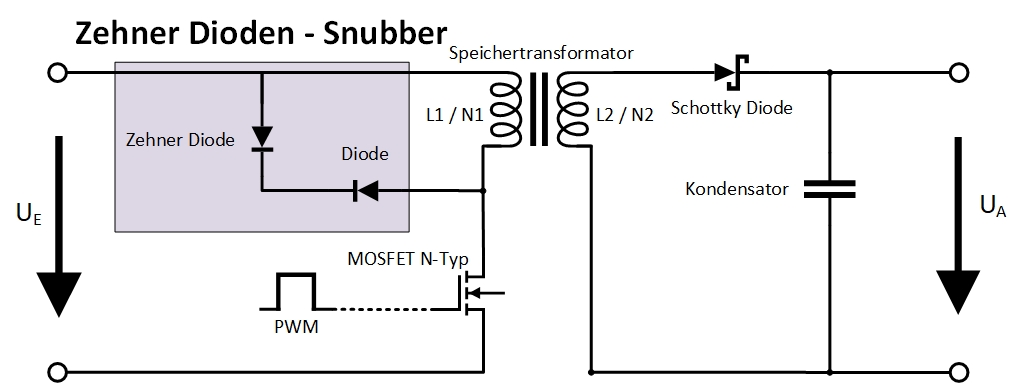
\includegraphics[width=0.9\linewidth]{Flyback_zehner}
	\caption{Snubberschaltung mit Zener- Diode}\label{fig:Flyback_zehner}
\end{figure}

Die zweite Snubber-Schaltung (Abbildung \ref{fig:Flyback_zehner}) besteht aus einer Zener-Diode und einer Diode. Die Drain-Spannung steigt nach dem Abschalten des MOSFET an, bis die Dioden leitend werden und die Streuinduktivität des Übertrags damit entladen. Die Differenz der reflektierten Ausgangspannung und der Zenerspannung bestimmt die Entladerate. Je schneller die Energie aus der Streuinduktivität abgebaut werden kann, desto besser ist der Wirkungsgrad. Die Werte der Dioden hängen von der zulässigen Spannungsbelastung des MOSFET ab. Nachdem die Streuinduktivität entladen ist, sollte die Z-Diode nicht mehr leiten. Aus diesem Grund sollte die Zenerspannung grösser als die reflektierte Ausgangsspannung sein. \textcolor{red}{[power-tipps 54]}

\subsection{Grundlagen zur Datenübertragung}
In diesem Unterkapitel werden einige Grundlagen zur Datenübertragung erläutert. Mittels dieser Grundlagen sollen die Eigenschaften des zu übertragenden Datenbussystems und Grundkenntnisse zu Photodioden und Empfängerschaltungen vermittelt werden. Es soll dem Leser als Basis für das Kapitel \textbf{\ref{sec:Daten} \nameref{sec:Daten}} dienen.

\paragraph{VARAN-Bus}
Der VARAN-Bus ist ein Echtzeit-Bussystem für die industrielle Automatisierung. Der Bus ist ein offener, herstellerunabhängiger Standard. Er verbindet Anlagen, Maschinen und Komponenten in der modernen Industrie. Das Bussystem arbeitet nach dem Manager-/Client-Prinzip. Weil der Manager die Kommunikation initialisiert, sind Paketkollisionen ausgeschlossen. Die Übertragungsschicht basiert auf dem Ethernet-Standard nach IEEE 802.3. Die verwendete 100TX-Standard-Ethernet-Technologie erlaubt eine maximale Übertragungsgeschwindigkeit von 100MBit pro Sekunde.\textcolor{red}{[Varan-bus.net]}

\paragraph{Ethernet}
Ethernet ermöglicht den kabelgebundenen Datenaustausch in Form von Datenframes zwischen Geräten in einem lokalen Netz. Dabei gibt es verschiedene Standards für unterschiedliche Übertragungsraten. Der 100Base-TX Standard (Fast Ethernet) des VARAN-Bus erlaubt eine maximale Datenrate von 100MBit/s. Statt der Manchesterkodierung, wie beim 10MBit/s-Ethernet, wird der effizientere 4B5B-Code eingesetzt. Dadurch wird eine Taktrückgewinnung aus dem Signal möglich. Durch eine zusätzliche MLT-3 Kodierung wird der Gleichspannungsanteil entfernt. \textcolor{red}{[itwissen.info]}

\paragraph{4B5B Code:}
Der Leitungscode 4B5B bildet vier Nutzdatenbits auf fünf Codebits ab. Dadurch erhöht sich die codierte Bitrate um 25\%. Beim verwendeten Ethernet-Standard beträgt die codierte Symbolrate somit 125MBit/s. Bei der Abbildung auf fünf Codebits werden lange '0'-oder '1'-Folgen vermieden. Dadurch wird die Taktrückgewinnung aus dem Signal verbessert. \textcolor{red}{[itwissen.info]}

\paragraph{MLT-3 Code:}
Multilevel Transmission Encoding (MLT-3) ist ein Leitungscode mit drei Spannungspegeln. Diese werden mit den Symbolen (+,\ 0,\ -) bezeichnet. Bei einer logischen '1' ändert sich der Spannungspegel nach der fixen Folge [0,\ +,\ 0,\ -]. Wird eine logische '0' übertragen, ändert sich der Zustand der Leitung nicht. Abbildung \ref{fig:MLT3code} zeigt eine beliebige Datenfolge mit der dazugehörigen MLT-3 Codierung. \textcolor{red}{[itwissen.info]}
\begin{figure}[h]
\centering
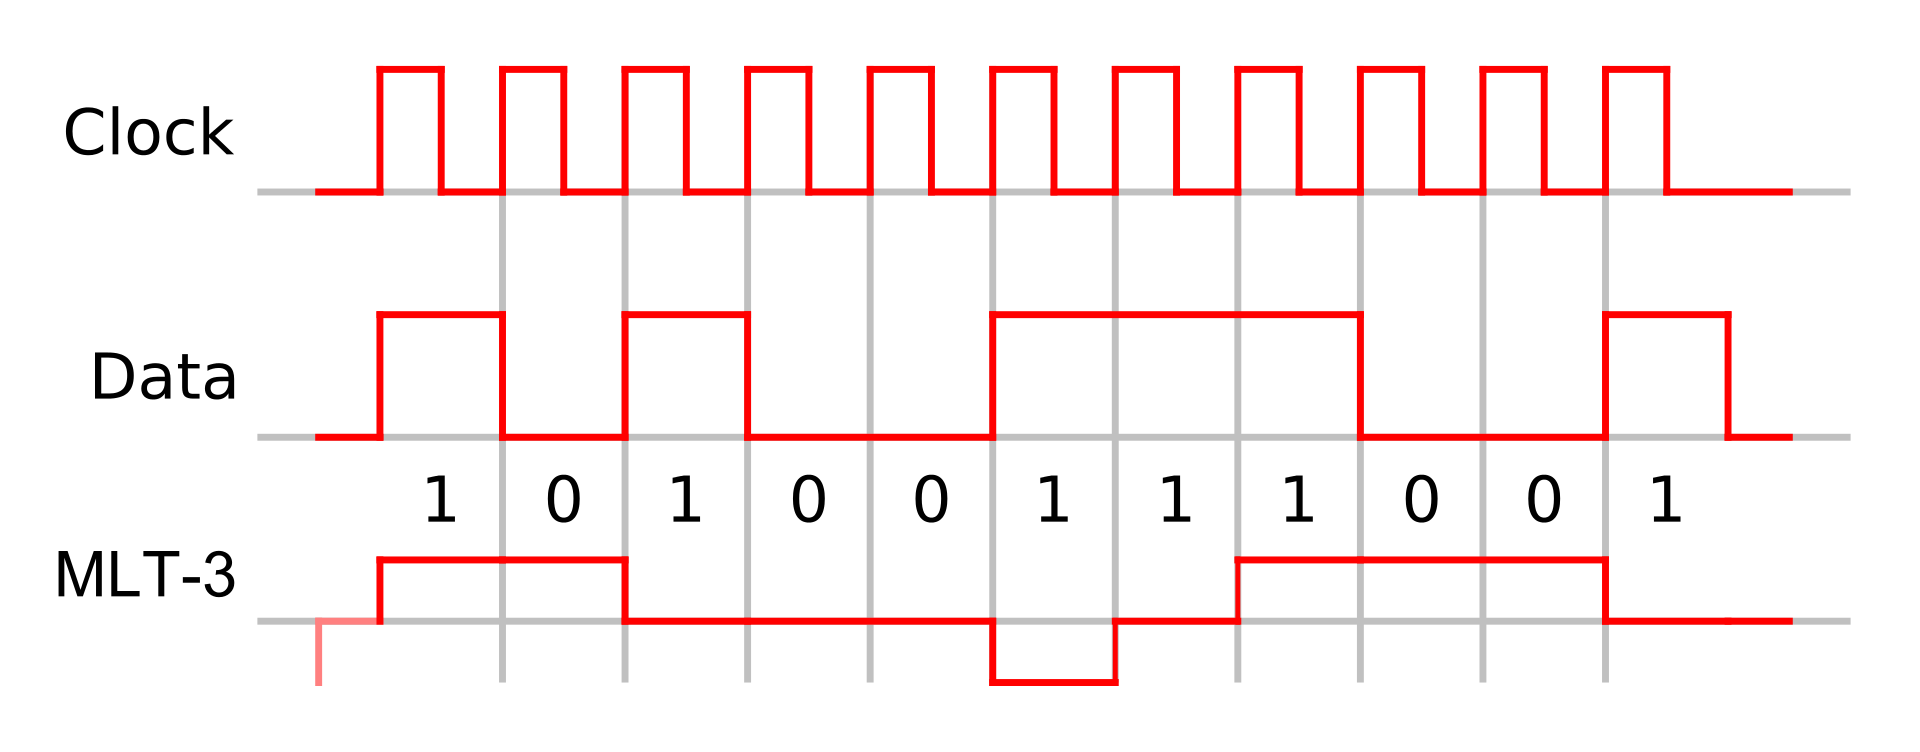
\includegraphics[width=0.8\linewidth]{MLT3encoding.png}
\caption{MLT-3 codierte Datenfolge}\label{fig:MLT3code}
\end{figure}

In einer Übertragungsschwingung werden 4 Bit übertragen. Damit reduziert sich die eigentliche Übertragungsfrequenz auf einen Viertel der Symbolrate. Die maximale Übertragungsfrequenz auf der Leitung beträgt demnach: 
\begin{equation}\label{eq:MLT3}
f_{max}=\frac{Symbolrate}{4 Bit}=\frac{125Mbit/s}{4 Bit}=31.25 MHz
\end{equation}
Um die Datenrate von \SI{100}{MBit/s} zu erreichen, dürften also \SI{31.25}{MHz} ausreichen.

\paragraph{Photodioden-Verstärker}
Photodioden sind Halbleiter-Dioden, die auftreffende Photonen in einen elektrischen Strom umwandeln. Abbildung \ref{fig:Kenn_Photodiode} zeigt die typische U-I-Kennlinie einer Photodiode.
\begin{figure}[h]
	\centering
	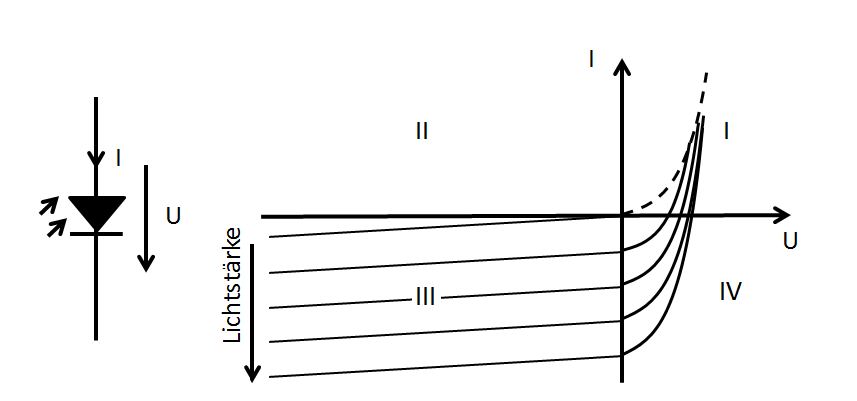
\includegraphics[width=0.8\linewidth]{Kennlinie_Photodiode.png}
	\caption{typische Kennlinie einer Photodiode}\label{fig:Kenn_Photodiode}
\end{figure}
Da im dritten Quadranten ein linearer Zusammenhang zwischen Lichtstärke und Photostrom erkennbar ist, eignet sich dieser Bereich für Sensoranwendungen und in unserem Fall auch Signalübertragungen.
Eine reale Photodiode besteht aus einer idealen Diode und einer parallel geschalteten Stromquelle. Der Strom ist abhängig von der Lichtstärke. Ein hochohmiger Widerstand stellt den Dunkelstrom der Photodiode dar. Die parasitäre Kapazität hängt primär von der Geometrie der Diode ab.
 \begin{figure}[H]
 	\centering
 	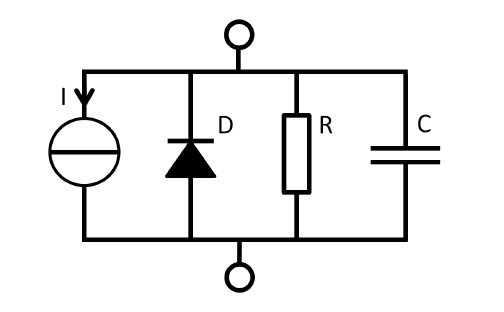
\includegraphics[width=0.8\linewidth]{Ersatzschaltbild_Photodiode.png}
 	\caption{Ersatzschaltbild einer Photodiode}\label{fig:Ersatz_Photodiode}
 \end{figure}
Für eine richtige Dimensionierung einer Schaltung, sind diese Parameter des Ersatzschaltbildes unbedingt zu beachten. Vor allem bei höheren Frequenzen hat die parasitäre Kapazität einen starken Einfluss. Der Widerstand ist normalerweise im Mega- oder Gigaohm-Bereich und kann vernachlässigt werden. \newline

Der Photostrom liegt meist im Nanoampere-Bereich und muss entsprechend verstärkt werden. Mit Hilfe eines Photodioden-Verstärkers wird der Photostrom in eine proportionale Spannung gewandelt. Meist werden dafür Transimpedanzverstärkerschaltungen eingesetzt.
\begin{figure}[h]
	\centering
	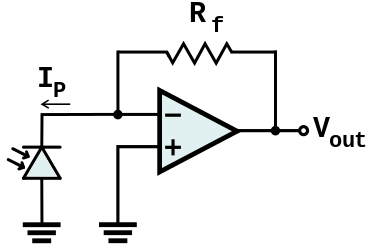
\includegraphics[width=0.5\linewidth]{Photo_Amp.png}
	\caption{Transimpedanzverstärker \textcolor{red}{[electronics.stackexchange]}}\label{fig:Photo_Amp}
\end{figure}

Da die Eingänge des Verstärkers hochimpedant sind, fliesst der Photostrom $ I_{p} $ nur durch den Rückkopplungswiderstand $ R_{f} $. Am Ausgang des Verstärkers stellt sich eine positive Spannung proportional zum Strom $ I_{p} $ ein. Die Ausgangsspannung beträgt:
\begin{equation}\label{eq:Vout_Photo}
V_{out}=R_{f} \cdot I_{p}
\end{equation}

Aus der Formel \ref{eq:Vout_Photo} ist leicht ersichtlich, dass $ R_{f} $ dem Verstärkungsfaktor der Transimpedanzverstärkerschaltung entspricht.

Die Bandbreite eines Photodiodenverstärkers ist begrenzt und hängt vom Gain-Bandwidth Product $GBWP$ des Operationsverstärkers, dem Rückkopplungswiderstand $ R_{f} $ und den parasitären Kapazitäten von Operationsverstärker $ C_{opamp} $ und Photodiode $ C_{photo} $ ab. Mit folgender Formel \ref{eq:Bandwidth} kann die Bandbreite berechnet werden:

\begin{equation}\label{eq:Bandwidth}
B=\sqrt{\frac{GBWP}{2\pi\cdot R_{f}\cdot (C_{opamp}+C_{photo})}}
\end{equation}

Wie man in der Formel erkennen kann, begrenzt unter anderem die Kapazität $ C_{photo} $ der Photodiode die Bandbreite der Schaltung. Durch Anlegen einer negativen Biasspannung an der Anode der Photodiode, kann $ C_{photo} $ reduziert werden.

Für eine Anwendung mit hoher Bandbreite, wie in dieser Arbeit verlangt, ist also ein Operationsverstärker mit hohem Gain-Bandwidth Product $GBWP$ und kleiner Eingangskapazität $ C_{opamp} $ gewünscht. Ausserdem wird idealerweise eine Photodiode mit kleiner parasitärer Kapazität $ C_{photo} $ verwendet und diese zusätzlich durch Anlegen einer negativen Biasspannung reduziert. \textcolor{red}{[schleuniger]}

\section{Energieübertagung}\label{sec:energie}
In diesem Kapitel wird aufgezeigt, wie die Energie übertragen werden soll. Zudem werden die Schaltung auf der Primär- und der Sekundärseite entworfen.

\subsection{Konzept}
In der Abbildung \ref{fig:konzept_energie} sind die wichtigsten Komponenten der induktiven Energieübertragung aufgeführt. Rot umrandet sind die Komponenten, die entwickelt werden müssen. Die Spannungsquelle und der Treiber für den Motor sind extern. Der Treiber bestimmt die zu übertragende Leistung von 300W und einer Gleichspannung von 48V.

\begin{figure}[h]
	\centering
	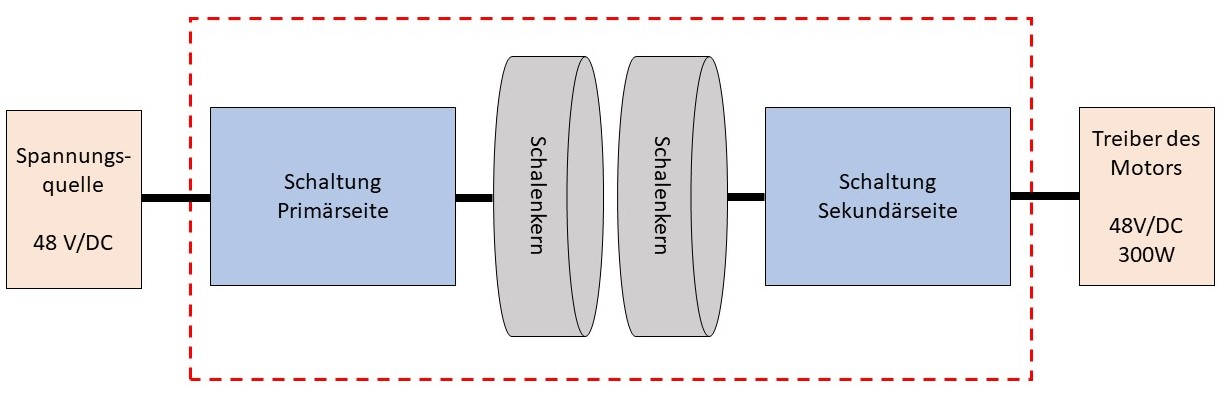
\includegraphics[width=1\linewidth]{konzept_energie}
	\caption{Konzept der induktiven Energieübertragung}\label{fig:konzept_energie}
\end{figure}

Die beiden Schalenkerne werden benötigt, um einen guten Kopplungsfaktor zu erreichen. Es sind Ferritkerne, welche aus dem Material BFM8 bestehen und eine Anfangspermeabilität $ \mu_{i} $ von 2400 aufweisen.\\ Die Schaltung auf der Primärseite hat die Aufgabe aus der Gleichspannung eine gepulste Spannung zu erzeugen, da keine konstante Spannung an der Spule anliegen darf. Wäre dies nicht der Fall, könnte man keine Energie übertragen. Denn das Magnetfeld der Spule würde sich nicht ändern und es würde kein Strom in der zweiten Spule induziert. \\
Auf der sekundären Seite wird wieder eine gepulste Spannung erhalten. Aus dieser gepulsten Spannung soll die Sekundärschaltung wieder eine Gleichspannung kreieren.

\paragraph{Auswahl der Schaltungstopologie}
Für die Energieübertragung kommen verschiedene Typologien zu Frage. Der Flyback bringt interessante Vorteile mit sich. Im Vergleich zu anderen Schaltungen, welche eine galvanische Trennung beinhalten, benötigt er weniger Bauteile. Zusätzlich eignet sich die Schaltung für einen Leistungsbereich bis zu ca. 500W. Im Gegensatz zum Resonanzwandler muss der benötigte Transformator bestimmte Anforderungen erfüllen, da er gleichzeitig als Energiespeicher eingesetzt wird. Da es für einen Prototypen von Vorteil ist möglichst wenig Bauteile zu verwenden, fiel der Entscheid auf den Flyback-converter.\textcolor{red}{[Speerwandler, bachelor]}

In der Abbildung \ref{fig:konzept_flyback} wird die Schaltung des Flyback-Converters aufgesplittet in die Primärschaltung, die Sekundärschaltung und die Schalenkerne. Die Primärseite besteht hauptsächlich aus dem MOSFET und dem Snubber-Glied. Die beiden Schalenkerne bilden den Speichertransformator, der für den Flyback benötigt wird. Die Sekundärschaltung ist ein Gleichrichter, welcher aus einer Schottky-Diode und einem Kondensator gebildet wird.
\begin{figure}[h]
	\centering
	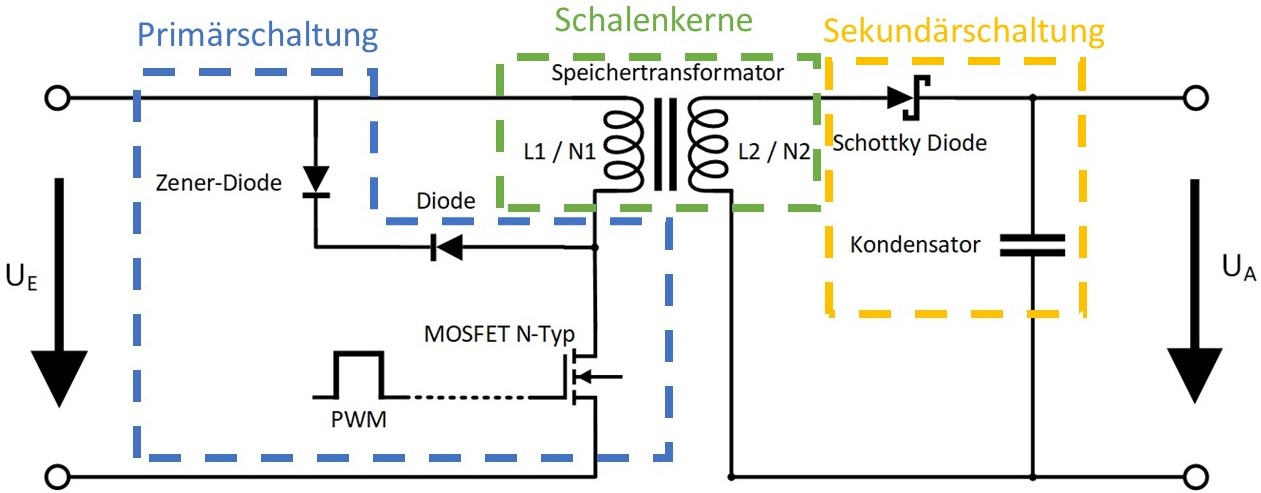
\includegraphics[width=0.9\linewidth]{konzept_flyback}
	\caption{Unterteilung der Flyback Schaltung}\label{fig:konzept_flyback}
\end{figure}


\subsection{Dimensionierung Flyback-Converter}

Um den Flyback-converter simulieren und später in einem Testaufbau realisieren zu können, müssen die wichtigsten Komponenten ausgelegt werden. In diesen Abschnitt wird die Dimensionierung der Induktivität des Speichertransformators, des MOSFET, der Schottky-Diode und der Snubber-Schaltung erklärt. Die genauere Dimensionierung des Speichertransformators wird im Abschnitt  \textbf{\ref{sec:simulation} \nameref{sec:simulation}} genauer beschrieben.

\paragraph{Berechnung der Induktivität}
Ein wichtiger Wert, um den Speichertransformator zu dimensionieren, ist die Induktivität. Mit den beiden Formeln \ref{eq:energie} und \ref{eq:Leistung} kann die übertragene Leistung $ P $ beschreiben werden. 

\begin{equation}\label{eq:zusammen}
P = \frac{1}{2} \cdot L \cdot \left (\frac{U_{E}}{L}\cdot a \cdot T_{p}\right ) ^{2} \cdot f_{p}
\end{equation}

Die Gleichung \ref{eq:zusammen} lässt sich nun nach der gesuchten Induktivität $ L $ umformen.

\begin{equation}\label{eq:induktivität}
L = \frac{a^{2}\cdot U_{E}\!^{2}\cdot T_{p}}{2 \cdot P}
\end{equation}

Mit einem Tastverhältnis $ a $ von 0.5, einer Eingangspannung $ U_{E} $ von 48V und der übertragenen Leistung $ P $ von 300W wird die Induktivität berechnet. Die Periodendauer $ T_{p} $ ist variabel.

\begin{equation}\label{eq:induktivität_berechnet}
L = \frac{0.5^{2}\cdot 48\mathrm{V}^{2}\cdot T_{p}}{2 \cdot 300\mathrm{W}}
\end{equation}

In der Tabelle \ref{tab:induktivität} sind die berechneten Resultate der Induktivität in Abhängigkeit zur Schaltfrequenz aufgeführt. Die Berechnungen geben Aufschluss darüber, dass die Induktivität kleiner werden muss, wenn die Frequenz erhört wird. Dies wird auch mit der Formel \ref{eq:strom} deutlich. In der Formel ist das Tastverhältnis, der Strom und die Spannung konstant. Wenn nun die Frequenz steigt, wird die Periodendauer kleiner und die Induktivität muss dementsprechend gesenkt werden.

\begin{table}[H]
	\centering
	\begin{tabular}{>{\tt}C{2.3cm}|  L{3cm}} 
		\normalfont\textbf{Frequenz} & \normalfont\textbf{Induktivität} \\ \hline\hline 
		10 kHZ & \SI{9.6e-05}{H}      \\ \hline
		20 kHZ & \SI{4.8e-05}{H}      \\ \hline
		30 kHZ & \SI{3.2e-05}{H}      \\ \hline
		40 kHZ & \SI{2.4e-05}{H}      \\ \hline
		50 kHZ & \SI{1.9e-05}{H}      \\ \hline
	\end{tabular}
\caption{Induktivität in Abhängigkeit der Schaltfrequenz }
\label{tab:induktivität}
\end{table}

\paragraph{Auslegung des MOSFET}
Die maximale Drain-Source-Spannung $ U_{DS} $ und der maximale Drain-Strom $ I_{D} $ sind wichtige Kenngrössen für die Auswahl des MOSFETs. Die grösste Spannung $ U_{DSmax} $, mit welcher der MOSFET belastet wird, berechnet sich mit der Formel \ref{eq:sperrspannung_mosfet}. Die Drain-Source-Spannung muss auf jeden Fall grösser $ U_{DSmax} $ gewählt werden.
\begin{equation}\label{eq:sperrspannung_mosfet}
U_{DSmax} = U_{e} + U_{a} \cdot \frac{N1}{N2}
\end{equation}
\begin{equation}\label{eq:sperrspannung_mosfet_berechnet}
U_{DSmax}= 48\mathrm{V} + 48\mathrm{V} \cdot 1 = 96\mathrm{V}
\end{equation}

\paragraph{Auslegung des Ausgangsdiode}
Die Sperrspannung $ U_{R} $ der Schottky-Diode muss folgendermassen ausgelegt werden.
\begin{equation}\label{eq:sperrspannung_diode}
U_{R} = U_{a} + U_{e} \cdot \frac{N2}{N1} = 48\mathrm{V} + 48\mathrm{V} \cdot 1 = 96\mathrm{V}
\end{equation}

\paragraph{Auslegung  Snubber Schaltung}
Im Kapitel \textbf{\ref{sec:Grundlagen} \nameref{sec:Grundlagen}} wurden zwei Snubber Schaltungen vorgestellt. Da der Aufbau mit einer Zener-Diode und einer Diode (Abbildung \ref{fig:Flyback_zehner}) effizienter und zusätzlich unabhängig von der Streuinduktivität ist, ist diese Topologie gewählt worden. Die Durchbruch-Spannung $ U_{Z} $ der Zener-Diode kann mit folgenden zwei Bedingungen festgelegt werden.  

\begin{equation}\label{eq:sperrspannung_zener1}
U_{Z} < U_{DS} - U_{E}
\end{equation}
\begin{equation}\label{eq:sperrspannung_zener1_berechnet}
U_{Z} <  150\mathrm{V} - 48\mathrm{V}  = 102\mathrm{V}
\end{equation}
\begin{equation}\label{eq:sperrspannung_zehner2}
U_{Z} > (U_{A} + U_{F}) \cdot \frac{N_{1}}{N_{2}}
\end{equation}
\begin{equation}\label{eq:sperrspannung_zehner2_berechnet}
U_{Z} >(48\mathrm{V} + 0.7\mathrm{V}) \cdot 1 = 48.7\mathrm{V}
\end{equation}
Die Durchbruch-Spannung darf also maximal 102 V betragen und mindestens 48.7 V.




\subsection{Simulation}\label{sec:simulation}
Um die dimensionierten Werte zu überprüfen und dementsprechend anzupassen, sind zwei Simulationen erstellt worden. Mit dem Simulationstool FEMM kann der Speichertrafo genauer betrachtet werden. Die Schaltung des Flyback-Converters ist im LTspice aufgebaut.

\paragraph{FEMM}
FEMM ist ein Simulationstool mit dem elektromagnetische Probleme im zweidimensionalen Bereich gelöst werden können. Der Speichertransformator ist im FEMM achsensymmetrisch aufgebaut. Er besteht aus den zwei Ferrit-Schalenkerne. Diese sind anhand des Datenblattes aufgezeichnet. Die Anfangspermeabilität $ \mu_{i} $ des Ferrits beträgt 2400 $ \frac{H}{m} $ und die Sätigungsflussdichte ist 490 mT. In der ersten Simulation wird ermittelt wie viele Windungen für den Speichertransformator benötigt werden. Mit der darauffolgende Simulation wird der Kopplungsfaktor berechnet.

Damit der Transformator mit der benötigten Induktivität aufgebaut werden kann, muss die Anzahl Windungen bekannt sein. Die Resultate der Simulation für verschiedene Frequenzen und Distanzen sind in der Tabelle \ref{tab:windungen} aufgeführt. Um die simulierten Werte zu vergleichen sind in der zweiten Spalte die berechneten Resultate aus der Tabelle \ref{tab:induktivität} eingetragen. Aus der Tabelle ist ersichtlich, dass bei konstanter Windungszahl sich die Induktivität bei ändernder Frequenz gleich bleibt.

\begin{table}[h]
	\centering
	\begin{tabular}{C{1.5cm} C{2.3cm}|C{2cm} C{2.3cm} |C{2cm} C{2.3cm} }
		\multicolumn{2}{c|}{\textbf{}} & \multicolumn{2}{c|}{\textbf{1mm Distanz}}
		& \multicolumn{2}{c}{\textbf{0.1mm Distanz}} \\
		{Frequenz}& {Berechnet} &{Windungen}& {Induktivität} & {Windungen}& {Induktivität}\\ \hline\hline
		\multirow{2}{*}{10 kHz}  & \multirow{2}{*}{\SI{9.6e-05}{H}} & 11 & \SI{8.17E-05}{H}  & 4 & \SI{7.45E-05}{H}  \\
							    							      & & 12 & \SI{9.72E-05}{H}  & 5 & \SI{1.16E-04}{H}  \\ \hline
		\multirow{2}{*}{20 kHz}  & \multirow{2}{*}{\SI{4.8e-05}{H}} & 8 & \SI{4.33E-05}{H}  & 3 & \SI{4.19E-05}{H}  \\
												 & & 9 & \SI{5.48E-05}{H}  & 4 & \SI{7.45E-05}{H}  \\ \hline
		\multirow{2}{*}{30 kHz}  & \multirow{2}{*}{\SI{3.2e-05}{H}} & 6 & \SI{2.44E-05}{H}  & 2 & \SI{1.87E-05}{H}  \\
												 & & 7 & \SI{3.32E-05}{H}  & 3 & \SI{4.19E-05}{H}  \\ \hline
		\multirow{2}{*}{40 kHz}  & \multirow{2}{*}{\SI{2.4e-05}{H}} & \multirow{2}{*}{6} & \multirow{2}{*}{\SI{2.44E-05}{H}}  & 2 & \SI{1.87e-05}{H}  \\
											     & &  &   & 3 & \SI{4.19E-05}{H}  \\ \hline
		\multirow{2}{*}{50 kHz}  & \multirow{2}{*}{\SI{1.9e-05}{H}} & 5 & \SI{1.70E-05}{H}  & \multirow{2}{*}{2} & \multirow{2}{*}{\SI{1.87E-05}{H}}  \\
												 & & 6 & \SI{2.44E-05}{H}  & &   \\ \hline
	\end{tabular}
	\caption{Resultate der Simulation in FEMM}\label{tab:windungen}
\end{table}

Mit dieser Simulation kann auch überprüft werden, ob der Ferritkern in Sättigung gerät. In der Abbildung \ref{fig:saettigung} ist das Resultat der Simulation des Ferritkerns mit 3 Windungen, einem Abstand von 0.1mm und einer Frequenz von 20kHz dargestellt. Wie man in der Abbildung erkennen kann, ist das B-Feld an den inneren Kecken am stärksten. An diesem Punkt hat das B-Feld einen Wert von ca. 344 mT. Damit der Ferritkern in Sättigung geraten würde braucht es eine Flussdichte von 490 mT. Dies bedeutet, dass der Kern nicht in Sättigung geht.

\begin{figure}[h]
	\centering
	\subfloat[B-Feld-Plot des Ferritkerns ]{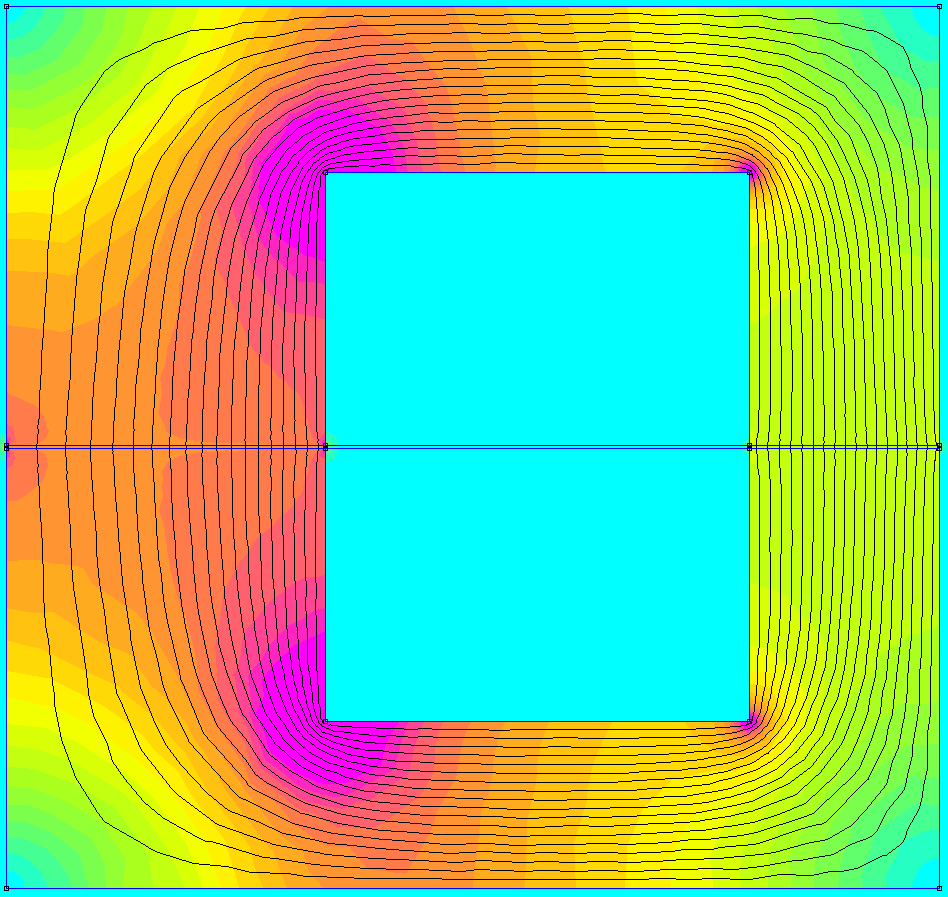
\includegraphics[width=0.45\linewidth]{saettigung_1}}\qquad
	\subfloat[Farbskala in Tesla]{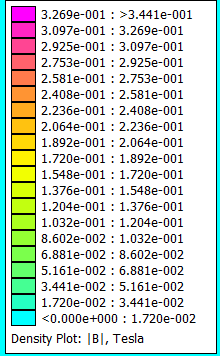
\includegraphics[width=0.25\linewidth]{saettigung_2}}
	\caption{Speichertransformator mit 0.1mm Abstand}
	\label{fig:saettigung}
\end{figure}
\newpage

Mit Hilfe der zweiten Simulation im FEMM soll der Koppelungsfaktor anhand der Formel \ref{eq:kopplungsfaktor} ermittelt werden. Um ihn berechnen zu können, benötigt man die Induktivitäten und die Gegeninduktivität.

\begin{figure}[H]
	\centering
	\subfloat[Strom durch primär Wicklung.]{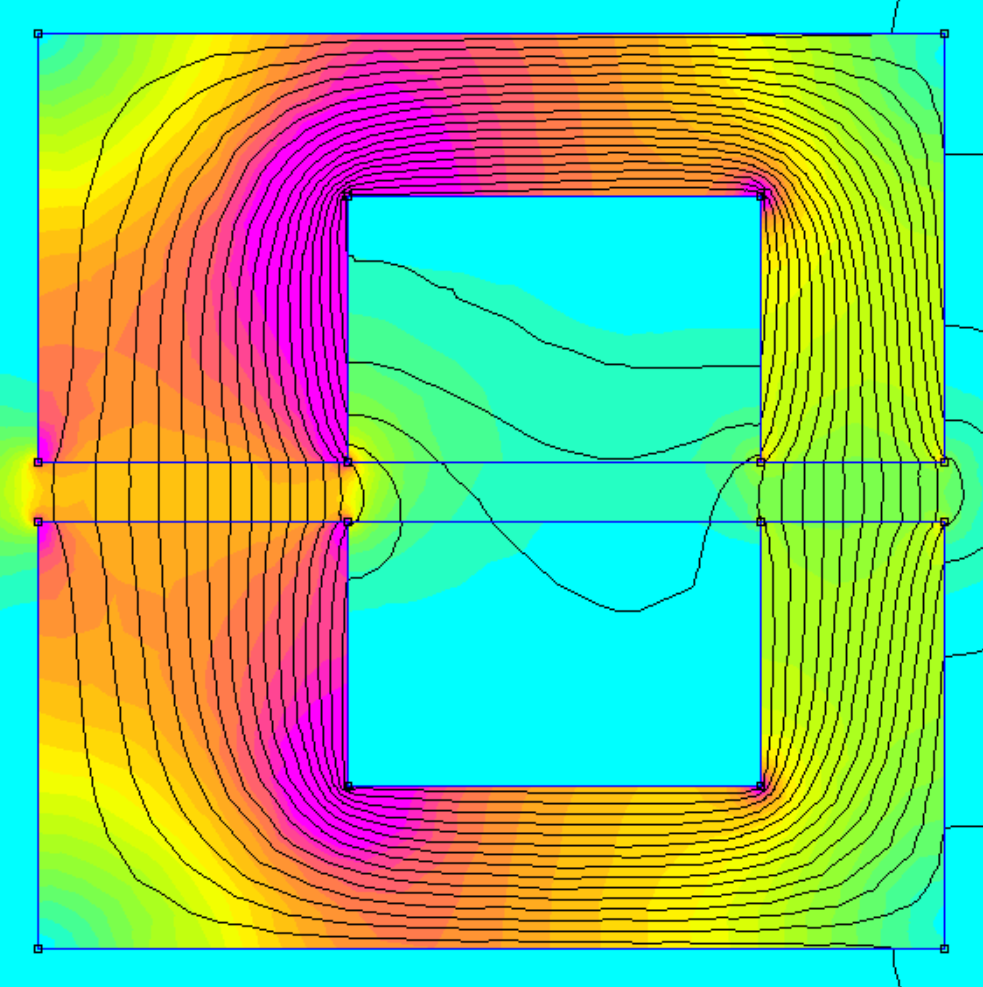
\includegraphics[width=0.45\linewidth]{femm_1.png}}\qquad
	\subfloat[Strom durch primär und sekundär Wicklung.]{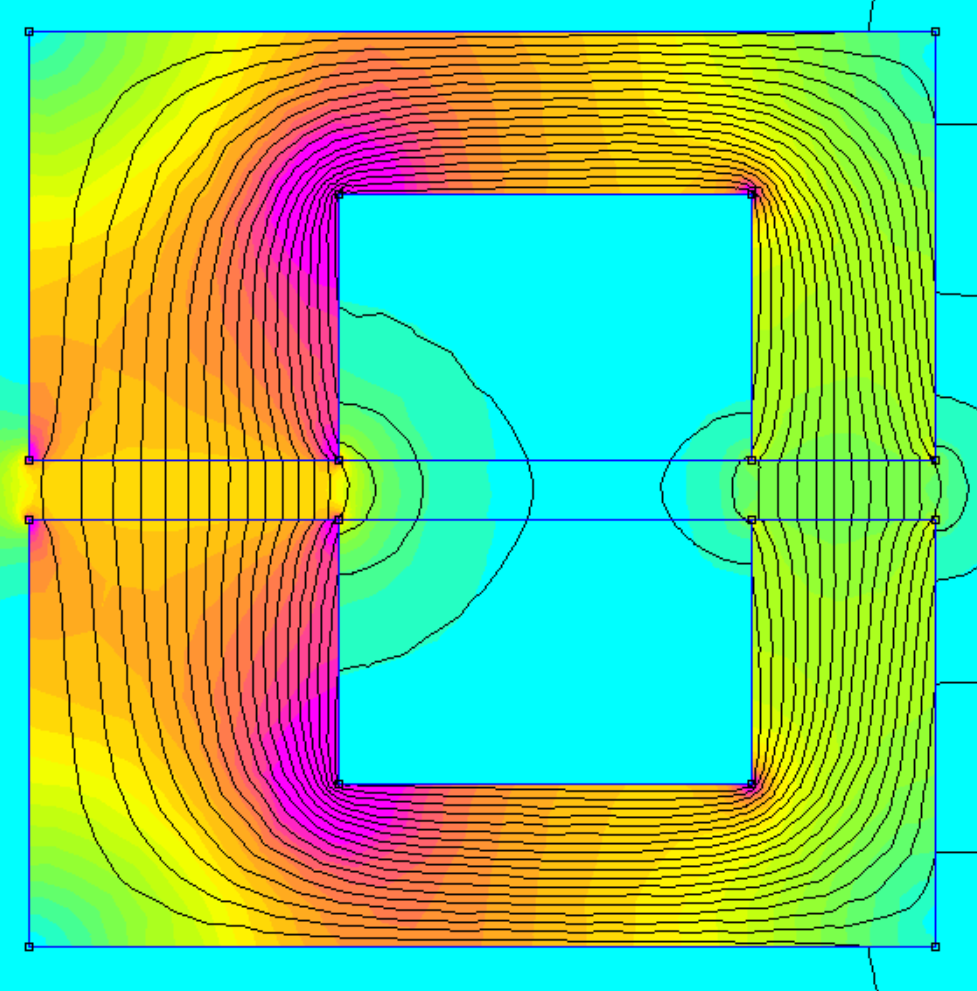
\includegraphics[width=0.45\linewidth]{femm_2.png}}
	\caption{Simulation des FEMM Models.}
	\label{fig:femmkopplung}
\end{figure}

In FEMM kann die Selbstinduktion der Primärspule simuliert werden, indem man einen Strom durch die Primär Wicklung lässt, wie in der Abbildung \ref{fig:femmkopplung}. Mit dem ermittelten Fluss $ \Psi_{11}  $ und dem Strom $ I_{1} $ kann die Induktivität $ L_{1} $ wie folgt berechnet werden. Das Simulationstool übernimmt diese Rechnung und kann die Induktivität direkt ausgeben.

\begin{equation}
L_{1}=\frac{\Psi_{11}}{I_{1}}
\label{eq:femm_l1}
\end{equation}

Mit der Formel \ref{eq:femm_M} wird die gesuchte Gegeninduktivität $ M $ berechnet.
Der dazu benötigte Fluss $ \Psi_{1} $ lässt sich in FEMM ermitteln indem man durch die Primär und Sekundär einen Strom fliesen lässt, wie in der Abbildung \ref{fig:femmkopplung}. 

\begin{equation}
M=\frac{\Psi_{1}-\Psi_{11}}{I_{1}}=\frac{\Psi_{12}}{I_{1}}
\label{eq:femm_M}
\end{equation}

Da $ L_{1} $ und $ L_{2} $ denselben Wert besitzen, kann man die Formel \ref{eq:kopplungsfaktor} vereinfachen, wodurch sich nun der Kopplungsfaktor $ k $ wie folgt definiert.

\begin{equation}
k=\frac{M}{\sqrt{L_{1}^{2}}}
\label{eq:kopplungsfaktor_neu}
\end{equation}

In der Tabelle \ref{tab:kopplung} sind die Resultate der Simulation eingetragen. In der letzten Spalte ist der Kopplungsfaktor mit der Formel \ref{eq:kopplungsfaktor_neu} berechnet. Die für die Berechnung benötigte Induktivität ist aus der Tabelle \ref{tab:windungen} aus der Spalte der simulierten Resultate entnommen worden. 

\begin{table}[h]
	\centering
	\begin{tabular}{>{\tt}C{2.0cm}| C{3cm} |  C{3cm} |  C{3cm} |  C{1.5cm}} 
		\normalfont\textbf{Frequenz} & \normalfont\textbf{Abstand} & \normalfont\textbf{$ \mathbf{\mathrm{\Psi_{11}}} $} & \normalfont\textbf{$ \mathbf{\mathrm{\Psi_{1}}} $} & \normalfont\textbf{k}\\ \hline\hline 
		\multirow{2}{*}{10 kHz} & \SI{0.1e-03}{m} & \SI{446.9e-06}{W} & \SI{889.2e-06}{W} &  \textbf{0.989}    \\ 
		& \SI{1e-03}{m} & \SI{583.3e-06}{W} & \SI{1100e-06}{W} & \textbf{0.934}     \\ \hline
		\multirow{2}{*}{20 kHz} & \SI{0.1e-03}{m} & \SI{ 251.5e-06}{W} & \SI{ 500.2e-06}{W} & \textbf{0.989}    \\ 
		       & \SI{1e-03}{m} & \SI{260e-06}{W}& \SI{502.1e-06}{W} &  \textbf{0.932}   \\ \hline
			\multirow{2}{*}{30 kHz} & \SI{0.1e-03}{m} & \SI{251.6e-06}{W} & \SI{500.4e-06}{W} & \textbf{0.988}     \\ 
		& \SI{1e-03}{m} & \SI{199.1e-06}{W} & \SI{384.5e-06}{W} &  \textbf{0.93}   \\ \hline
			\multirow{2}{*}{40 kHz} & \SI{0.1e-03}{m} & \SI{112.1e-06}{W} & \SI{222.7e-06}{W} &  \textbf{0.986}    \\ 
		& \SI{1e-03}{m} & \SI{146.5e-06}{W} & \SI{282.7e-06}{W} & \textbf{0.929}     \\ \hline
			\multirow{2}{*}{50 kHz} & \SI{0.1e-03}{m} & \SI{112.1e-06}{W} & \SI{222.7e-06}{W} &  \textbf{0.986}    \\ 
		& \SI{1e-03}{m} &\SI{102.02e-06}{W} & \SI{196.56e-06}{W}&  \textbf{0.926}   \\ \hline
	\end{tabular}
	\caption{Induktivität in Abhängigkeit der Schaltfrequenz }
	\label{tab:kopplung}
\end{table}

Der Kopplungsfaktor k beträgt etwas mehr als 0.9. Er wird grösser indem die Induktivität erhöht wird. Der beste Kopplungsdoktor ist daher bei der Frequenz 10kHz und einem Abstand von 0.1mm. 



\paragraph{Schaltung}
Das Ziel der Simulation ist es, verschiedene Erkenntnisse über die Schaltung des zu erhalten wie der Wirkungsgrad, die Ausgangsstrom oder die Ausgangsspannung. Die Schaltung ist im LTspice aufgebaut. Die Bauteile, welche für den Flyback-converter benötigt werden, wurden anhand der Dimensionierung ausgesucht.

Der Speichertransformator wurde für 20kHz ausgelegt. Dies bringt mehrere Vorteile mit sich. Als erstes hört man diese Frequenz nicht mehr, was das Arbeiten mit dem Testaufbau einiges angenehmer macht. Beim Abstand von 0.1mm hat die berechnete Induktivität fast die kleinste Differenz zur simulierten Induktivität einer ganzen Windung. Als letztes hat die Spule nicht nur zwei Windungen und bietet etwas mehr Flexibilität.

Der Widerstand kann mit der Formel \ref{eq:Leistung} berechnet werden indem sie nach R umgeformt wird. 

\begin{equation}\label{eq:Widerstand}
R= \frac{U_{2}\!^{2}}{P}=\frac{48^{2}V}{300 W} = 7.68\Omega
\end{equation}

In der Abbildung \ref{fig:LT_schema} ist der Flyback-converter mit einer Zener-Snubber-Schaltung aufgebaut. Mit dieser Schaltung sind die nachfolgenden Simulationen durchgeführt worden.

\begin{figure}[H]
	\centering
	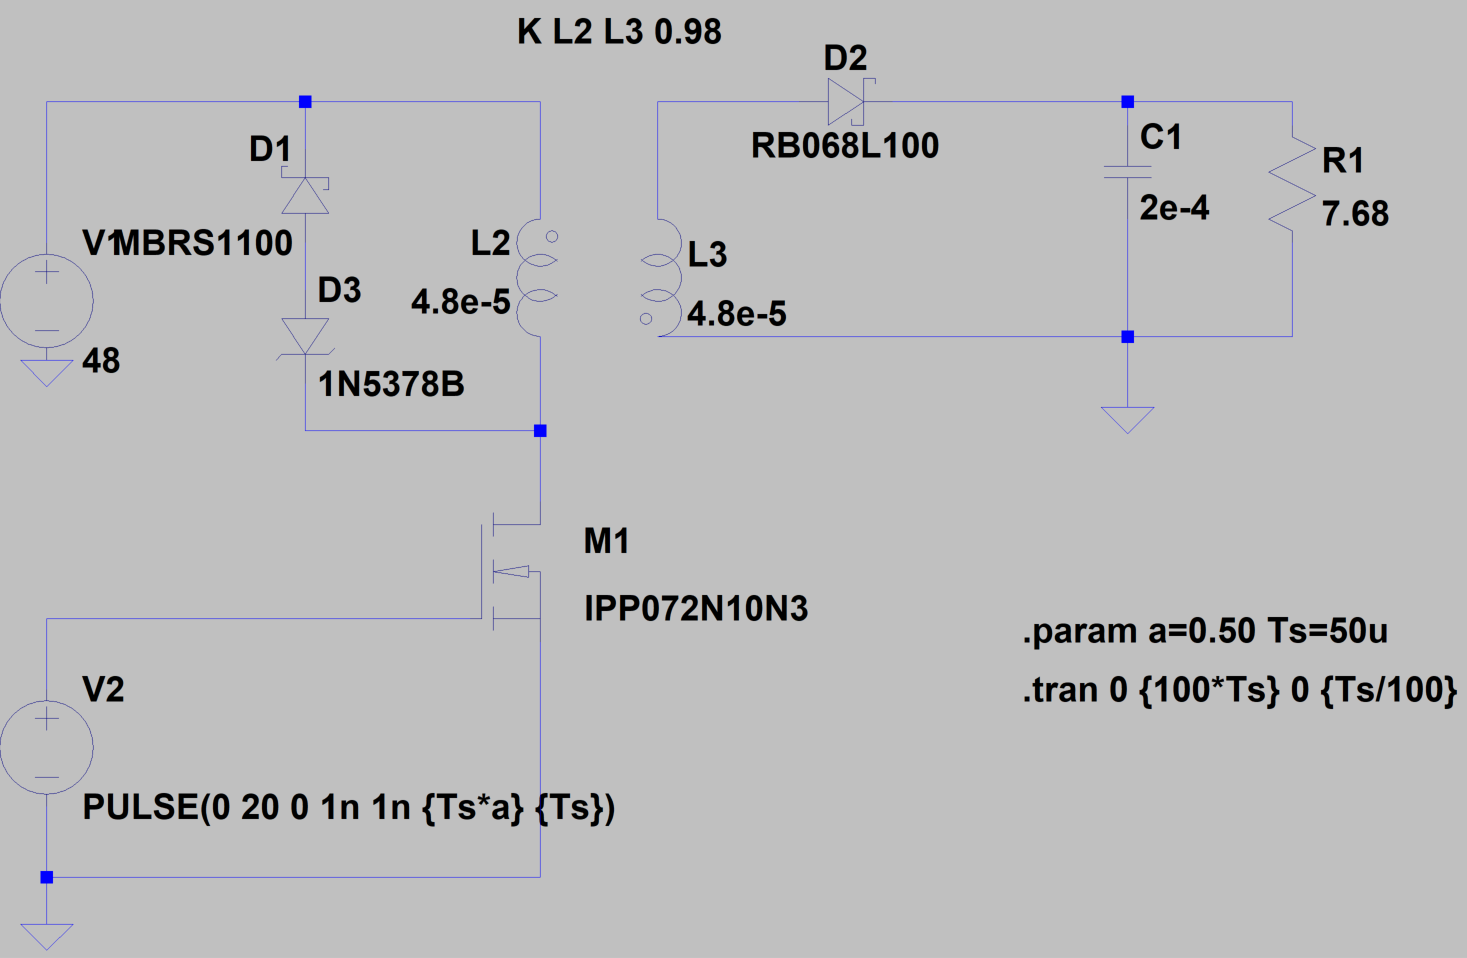
\includegraphics[width=1\linewidth]{LT_schaltung}
	\caption{Flyback-conveter im LTspice}\label{fig:LT_schema}
\end{figure}

Der Strom und die Spannung am Widerstand R1 sind in der Abbildung \ref{fig:ausgangsstrom} simuliert. Der Mittelwert und der RMS-Wert sind in der Tabelle \ref{tab:ausgang} eingetragen.

\begin{table}[h]
	\centering
	\begin{tabular}{>{\tt}C{2.3cm}|  C{3cm}|  C{3cm}} 
		\normalfont\textbf{Grösse} & \normalfont\textbf{Mittelwert} & \normalfont\textbf{RMS-Wert} \\ \hline\hline 
		Spannung & 47.6V & 48.4V   \\ \hline
		Strom & 6.2A &   6.3A   \\ \hline
		Leistung & 304.98W &      \\ \hline
	\end{tabular}
	\caption{Resultate der Simulation}
	\label{tab:ausgang}
\end{table}

Die Schaltung hat einen Wirkungsgrad von 52\% und lässt sich wie folgt berechne. 

\begin{equation}\label{eq:wirkungsgrand}
\eta=\frac{P_{ab}}{P_{zu}}=\frac{304.79W}{585.52W} = 0.52
\end{equation}

\begin{figure}[H]
	\centering
	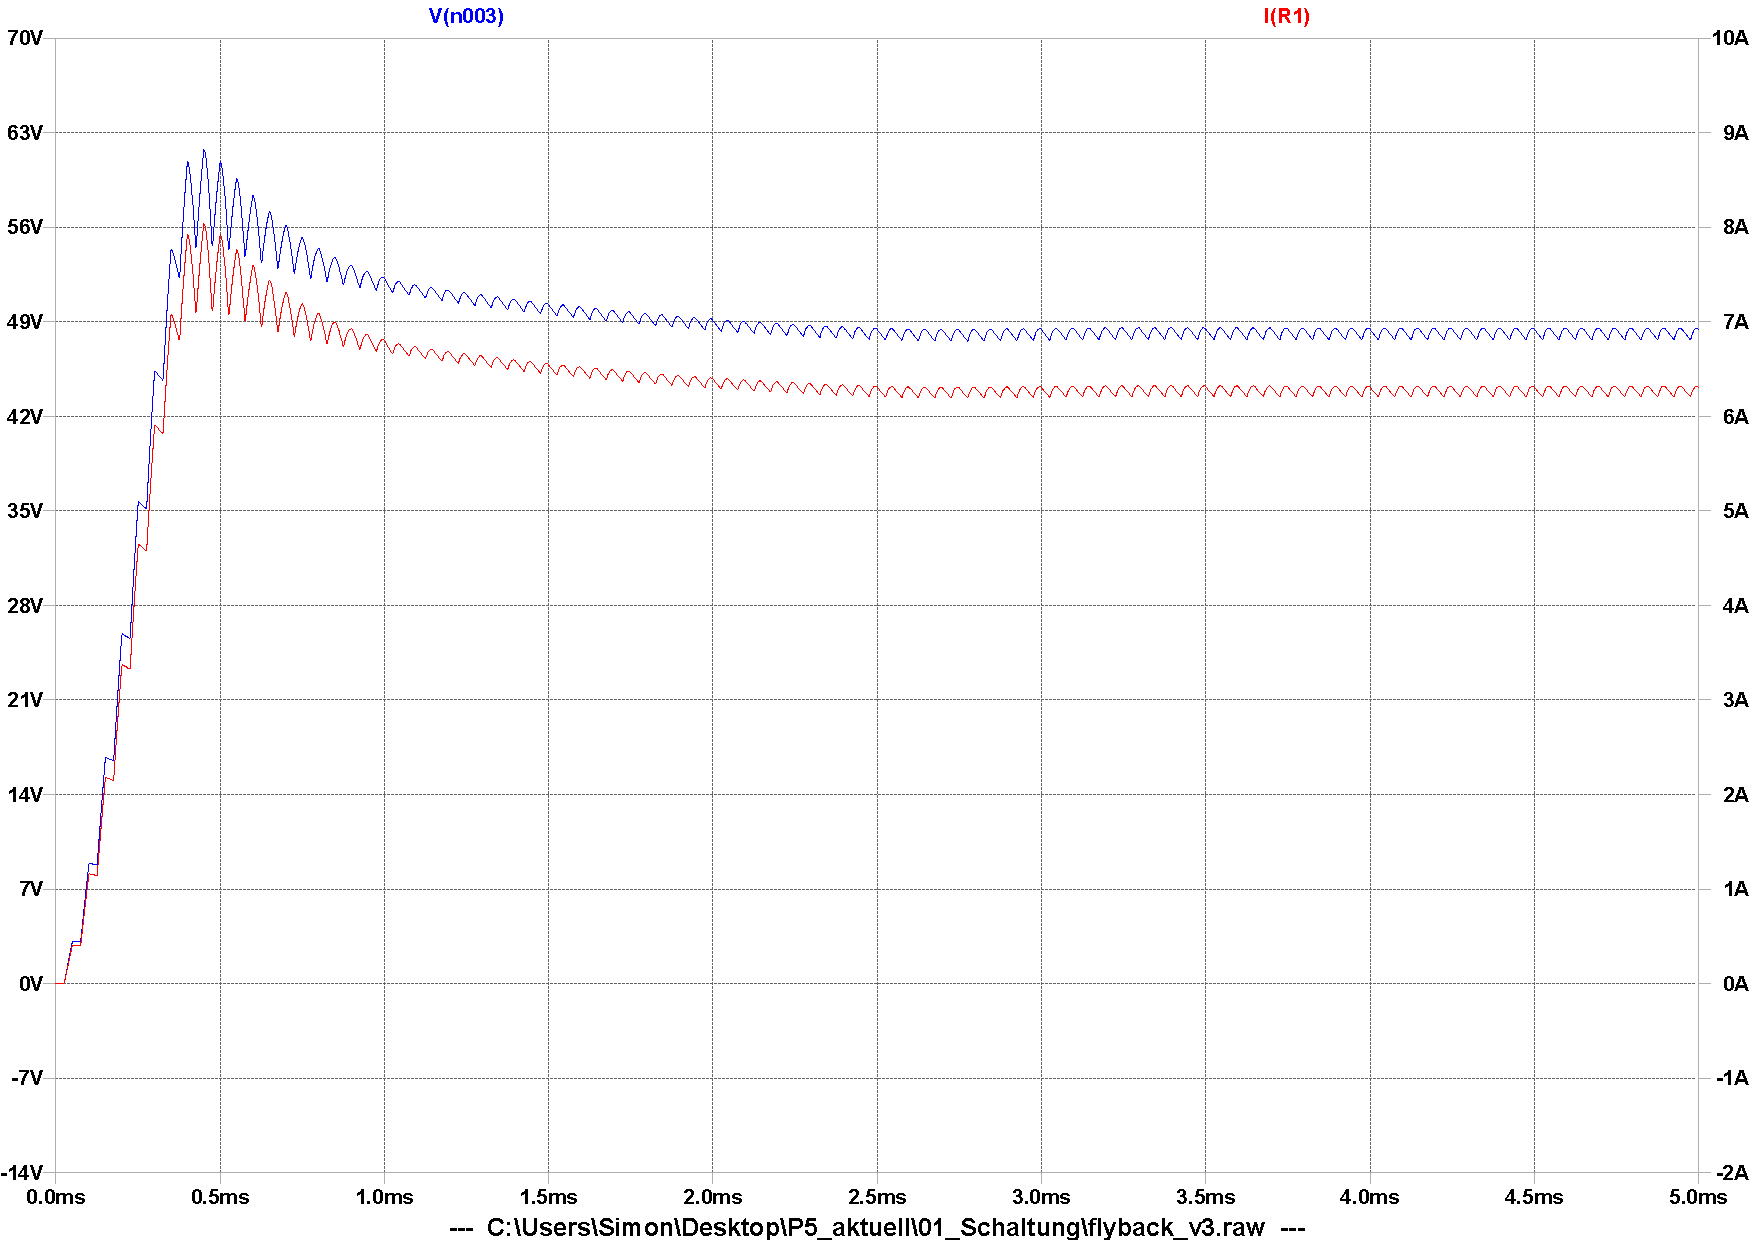
\includegraphics[width=0.8\linewidth]{flyback_v3_spannung}
	\caption{Storm () und Spannung () über dem Widerstand R1 }\label{fig:ausgangsstrom}
\end{figure}

Der Strom in der Spule L1 und der in Storm der Spule L2 mit dem PWM-Signal sind in der Abbildung \ref{fig:spule} dargestellt. Dieser Plot kann mit der Abbildung \ref{fig:kurven} verglichen werden. Zusätzlich ist die Spannung über der Spule L1 ist im Plot b abgebildet.

\begin{figure}[H]
	\centering
	\subfloat[B-Feld-Plot des Ferritkerns ]{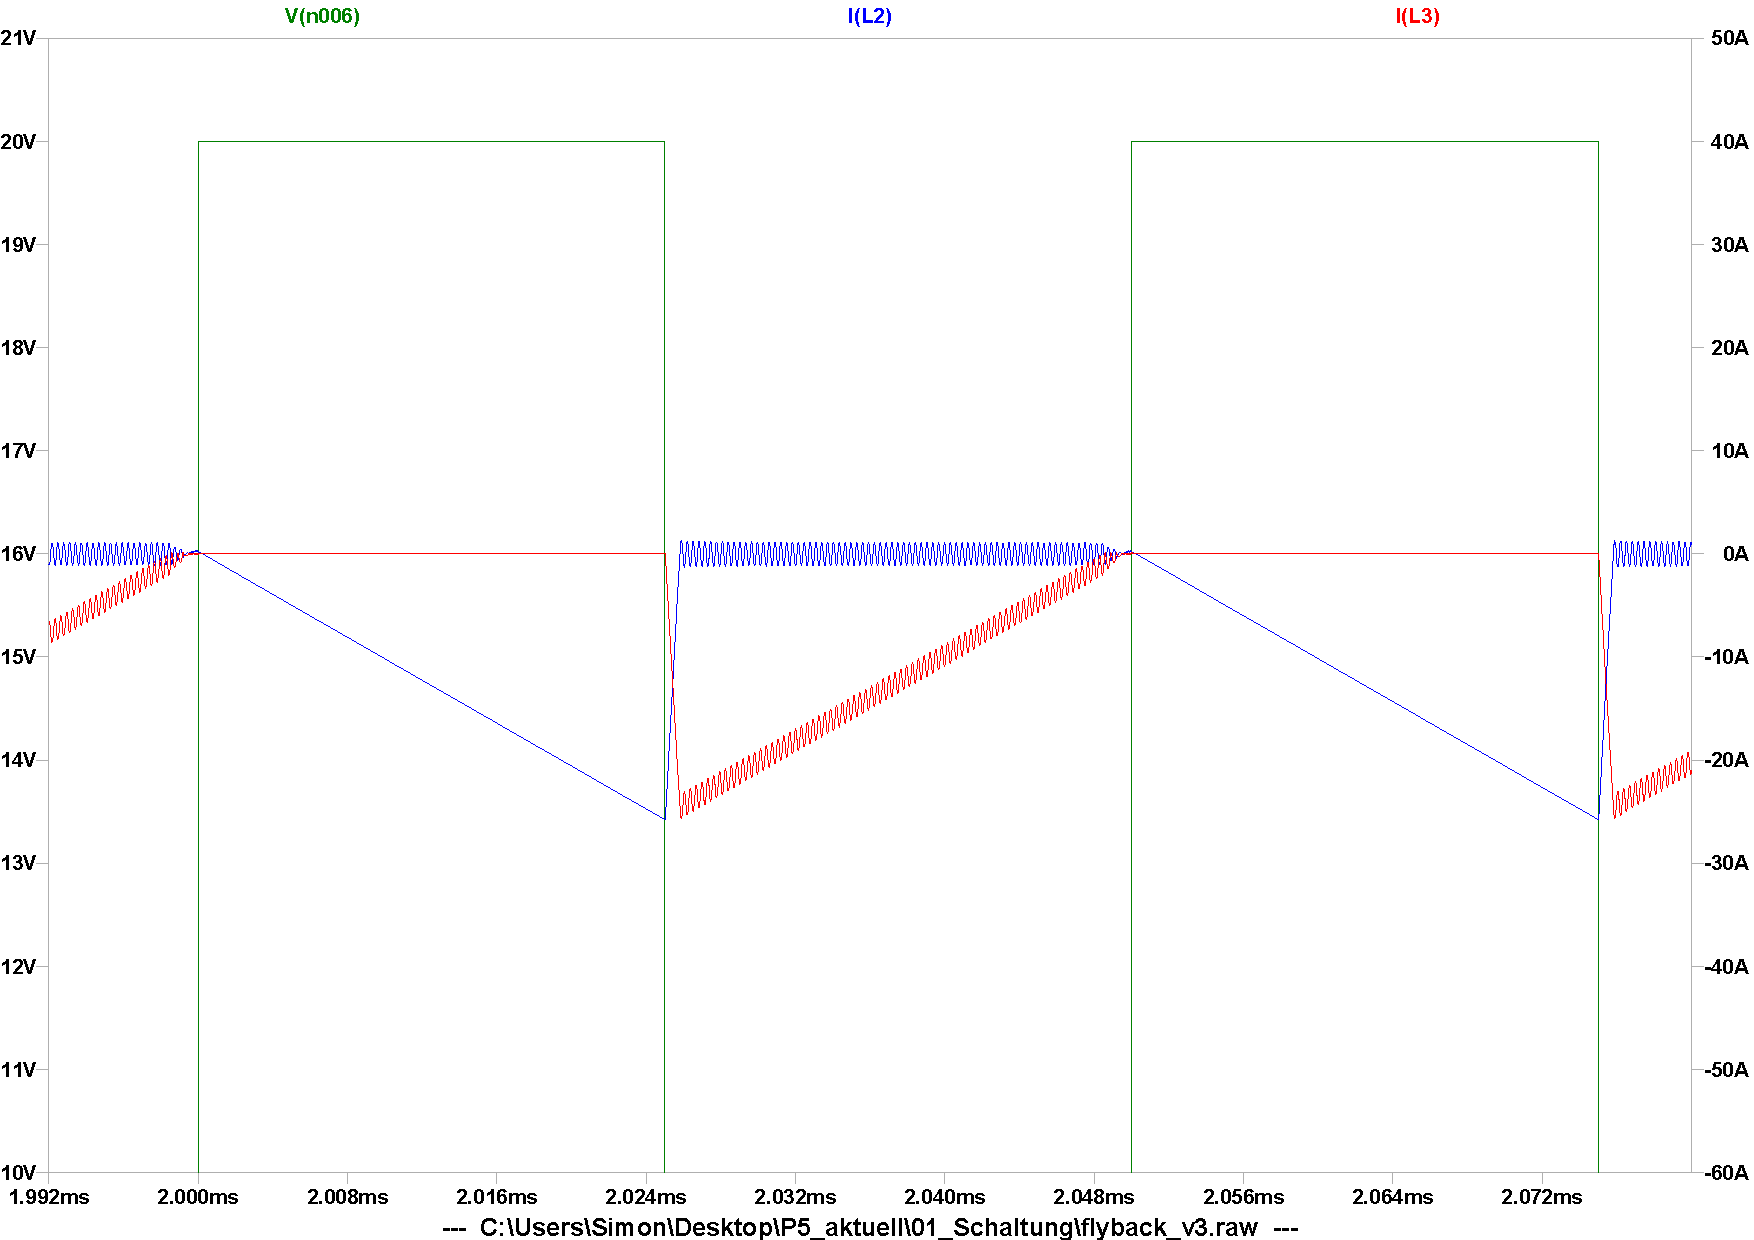
\includegraphics[width=0.7\linewidth]{flyback_v3_spule1}}\qquad
	\subfloat[Farbskala in Tesla]{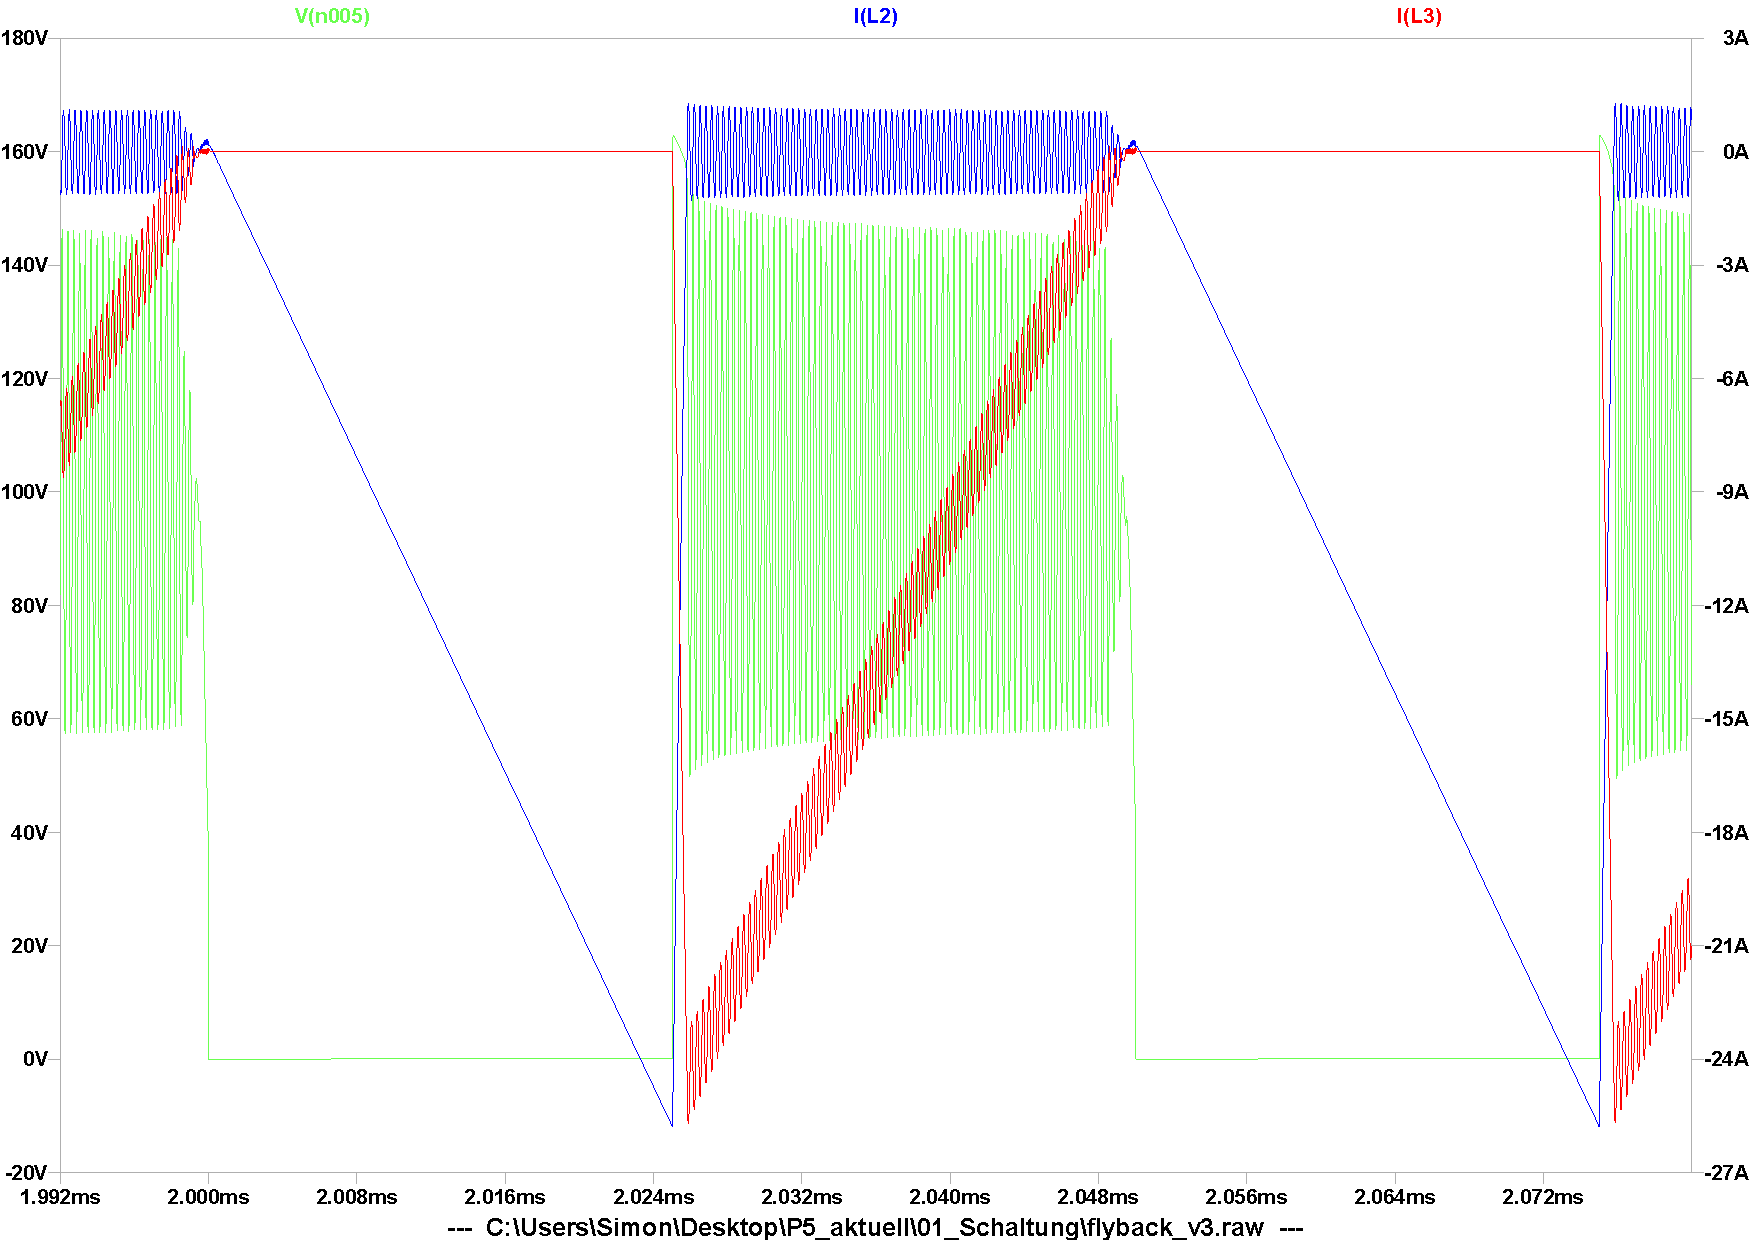
\includegraphics[width=0.7\linewidth]{flyback_v3_spule2}}
	\caption{Speichertransformator mit 0.1mm Abstand}
	\label{fig:spule}
\end{figure}

In der Abbildung wird der Strom und die Spannung über der Spule mit und ohne Snubber verglichen.

\begin{figure}[H]
	\centering
	\subfloat[B-Feld-Plot des Ferritkerns ]{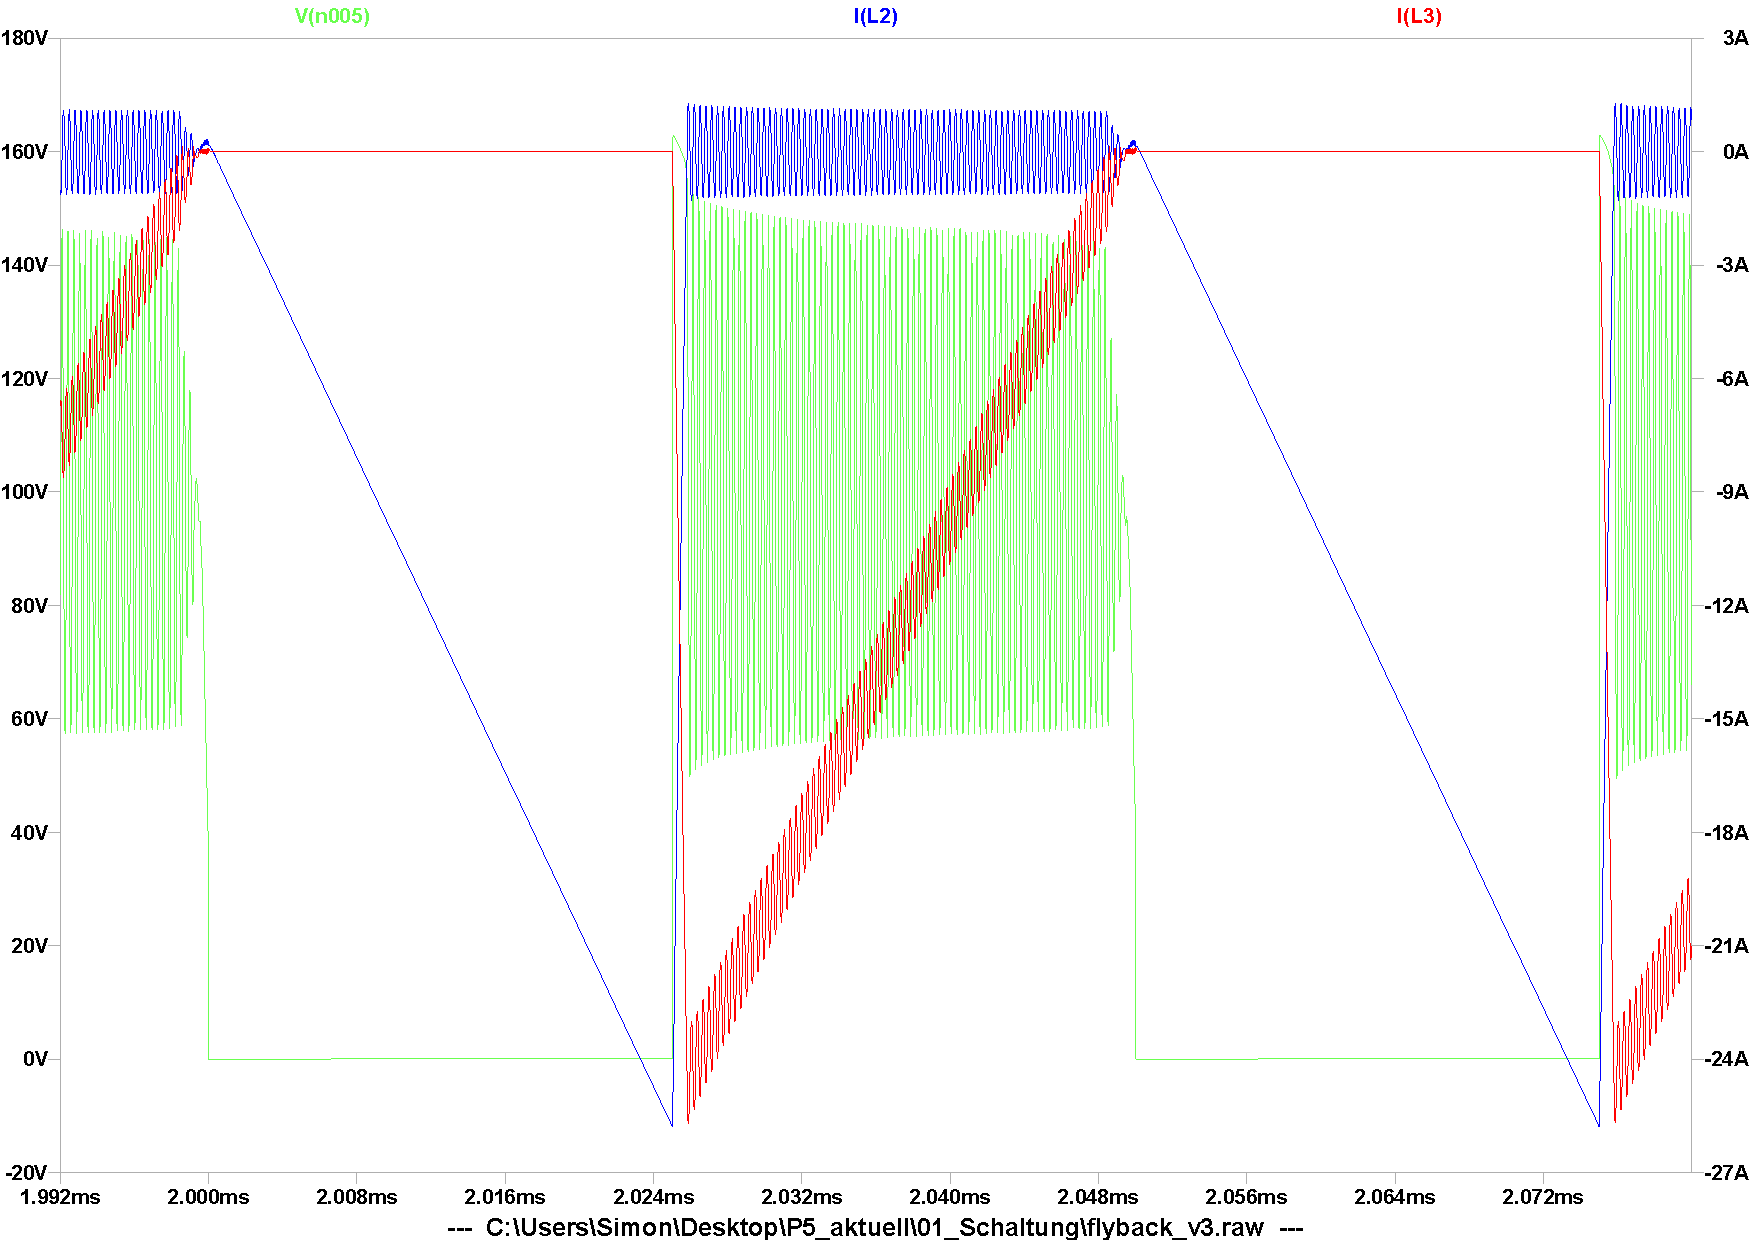
\includegraphics[width=0.6\linewidth]{flyback_v3_spule2}}\qquad
	\subfloat[Farbskala in Tesla]{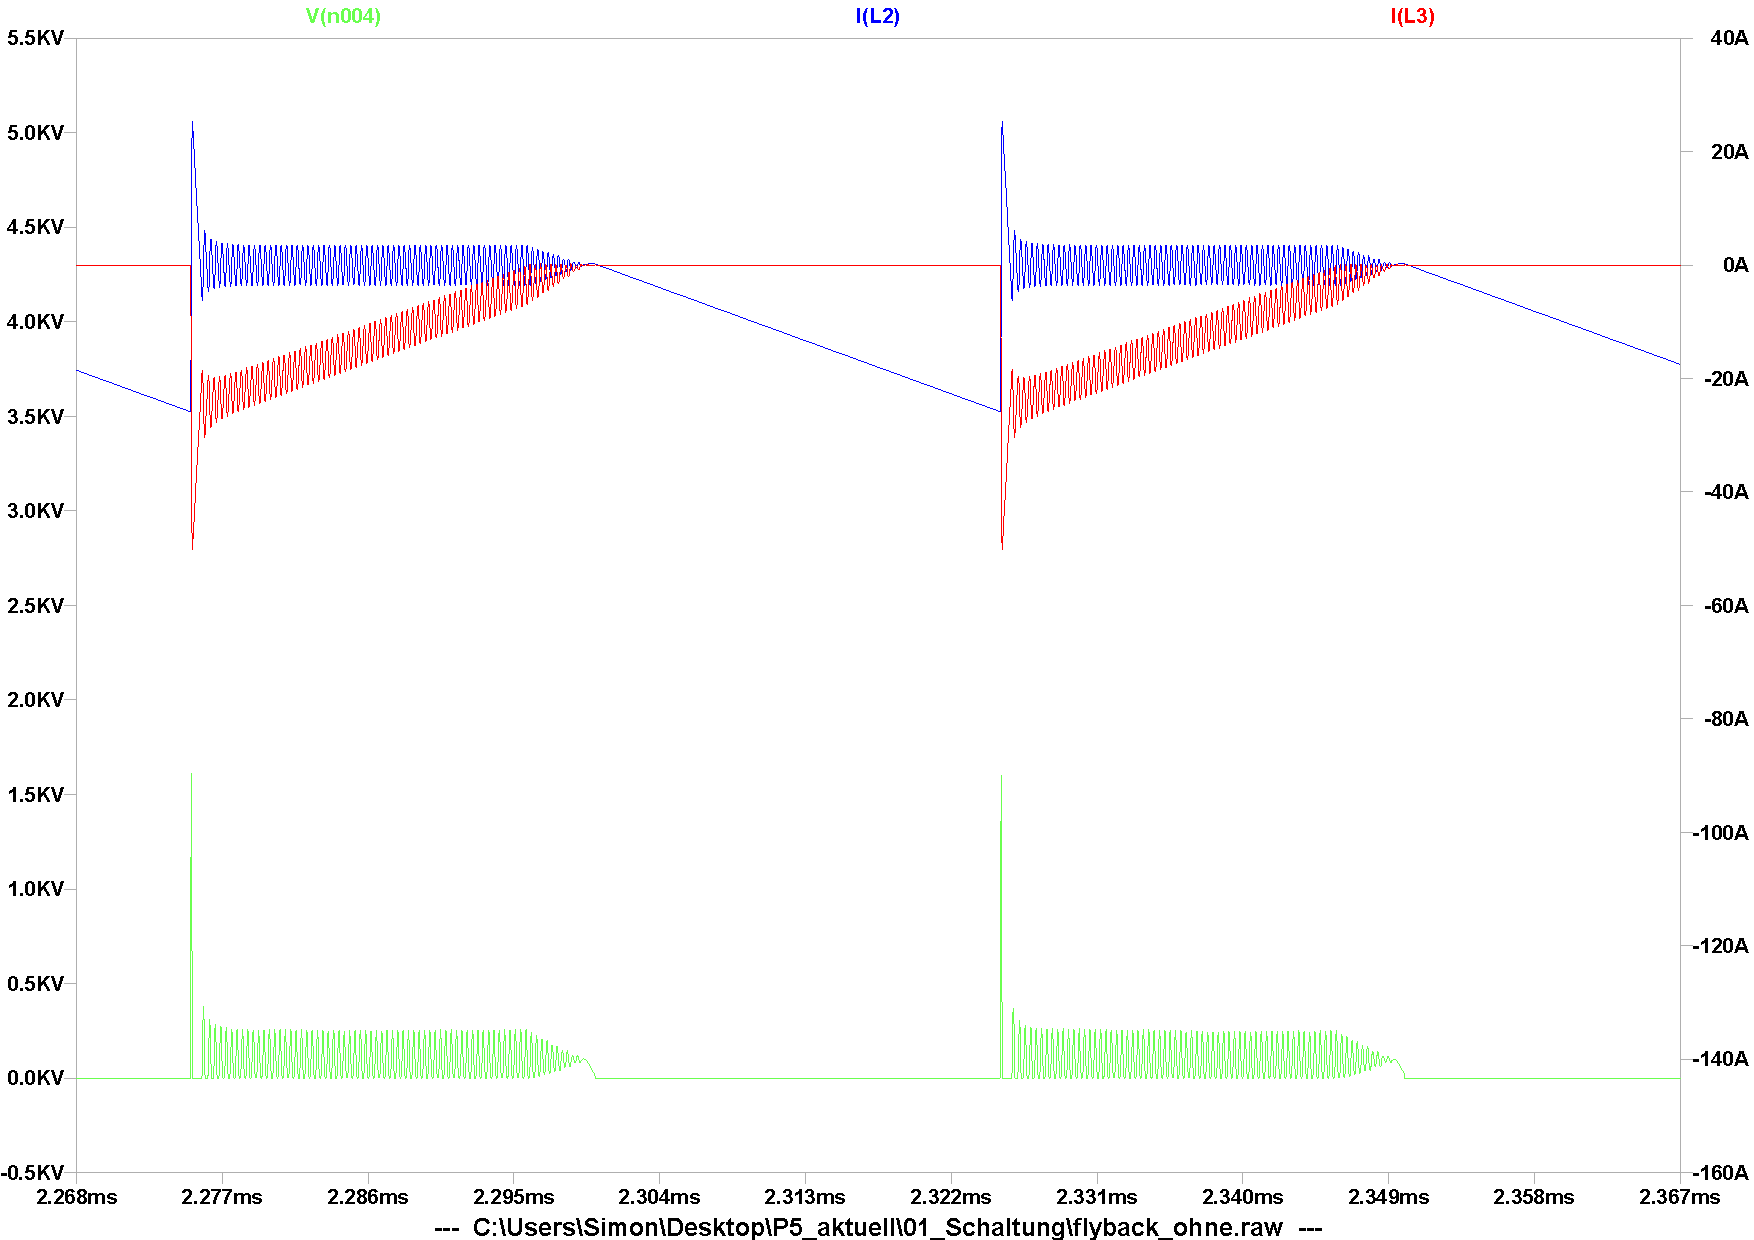
\includegraphics[width=0.6\linewidth]{flyback_ohne}}
	\caption{Speichertransformator mit 0.1mm Abstand}
	\label{fig:LT_snubber}
\end{figure}

Mit der Simulation in LTspice kann auch die Verlustleistung der Halbleiter ermittelt werden. Die Resultate sind in der Tabelle aufgeführt.

\begin{table}[h]
	\centering
	\begin{tabular}{>{\tt}C{2.3cm}| C{6cm}} 
		\normalfont\textbf{Bauteil} & \normalfont\textbf{Mittlere Verlustleistung} \\ \hline\hline 
		MOSFET M1 & 3.84W  \\ \hline
		Diode D1 & 197mW  \\ \hline
		Diode D2 & 26.47W \\ \hline
		Z-Diode D3 & 23.16W  \\ \hline
	\end{tabular}
	\caption{Resultate der Simulation}
	\label{tab:LT_verlsutleistung}
\end{table}

\subsection{Testaufbau}
\todo[inline]{Messung Induktivität, Widerstand, Freqeunzabhängig?}

\todo[inline]{Wirkungsgrad}
\todo[inline]{Energie}
\todo[inline]{Strom, Spannung}
\todo[inline]{Aufzeigen von Snubber}
\todo[inline]{Verlustleistung}

\subsection{Validierung}
Zur Energieübertragung wird der Kopplungsfaktor und die zu übertragene Leistung validiert. Auch der erreichte Wirkungsgrad wird betrachtet.

\todo[inline]{Vergleichen der Induktivität}
\todo[inline]{Vergleichen Kopplungsfaktor?}

\todo[inline]{Vergleichen der Schaltungssimulation - Realität:}
\todo[inline]{-Wirkungsgrad}
\todo[inline]{-Energie}
\todo[inline]{-Strom, Spannung}
\todo[inline]{-Aufzeigen von Snubber}
\todo[inline]{-Verlustleistung}
\section{Datenübertragung}
\label{sec:Daten}
Im folgenden wird ein Konzept beschrieben, um Daten des VARAN-Buses optisch und bidirektional zu übertragen. Ausserdem wird eine Sende- und Empfängerschaltung entworfen, um einen Teilbereich des Konzepts zu überprüfen und wichtige Erkenntnisse für die Fortsetzung der Arbeit zu sammeln.  
\subsection{Konzept}
In Abbildung \ref{fig:Konzept_Daten} wird grob das Konzept zur optischen Datenübertragung gezeigt.

\begin{figure}[h]
	\centering
	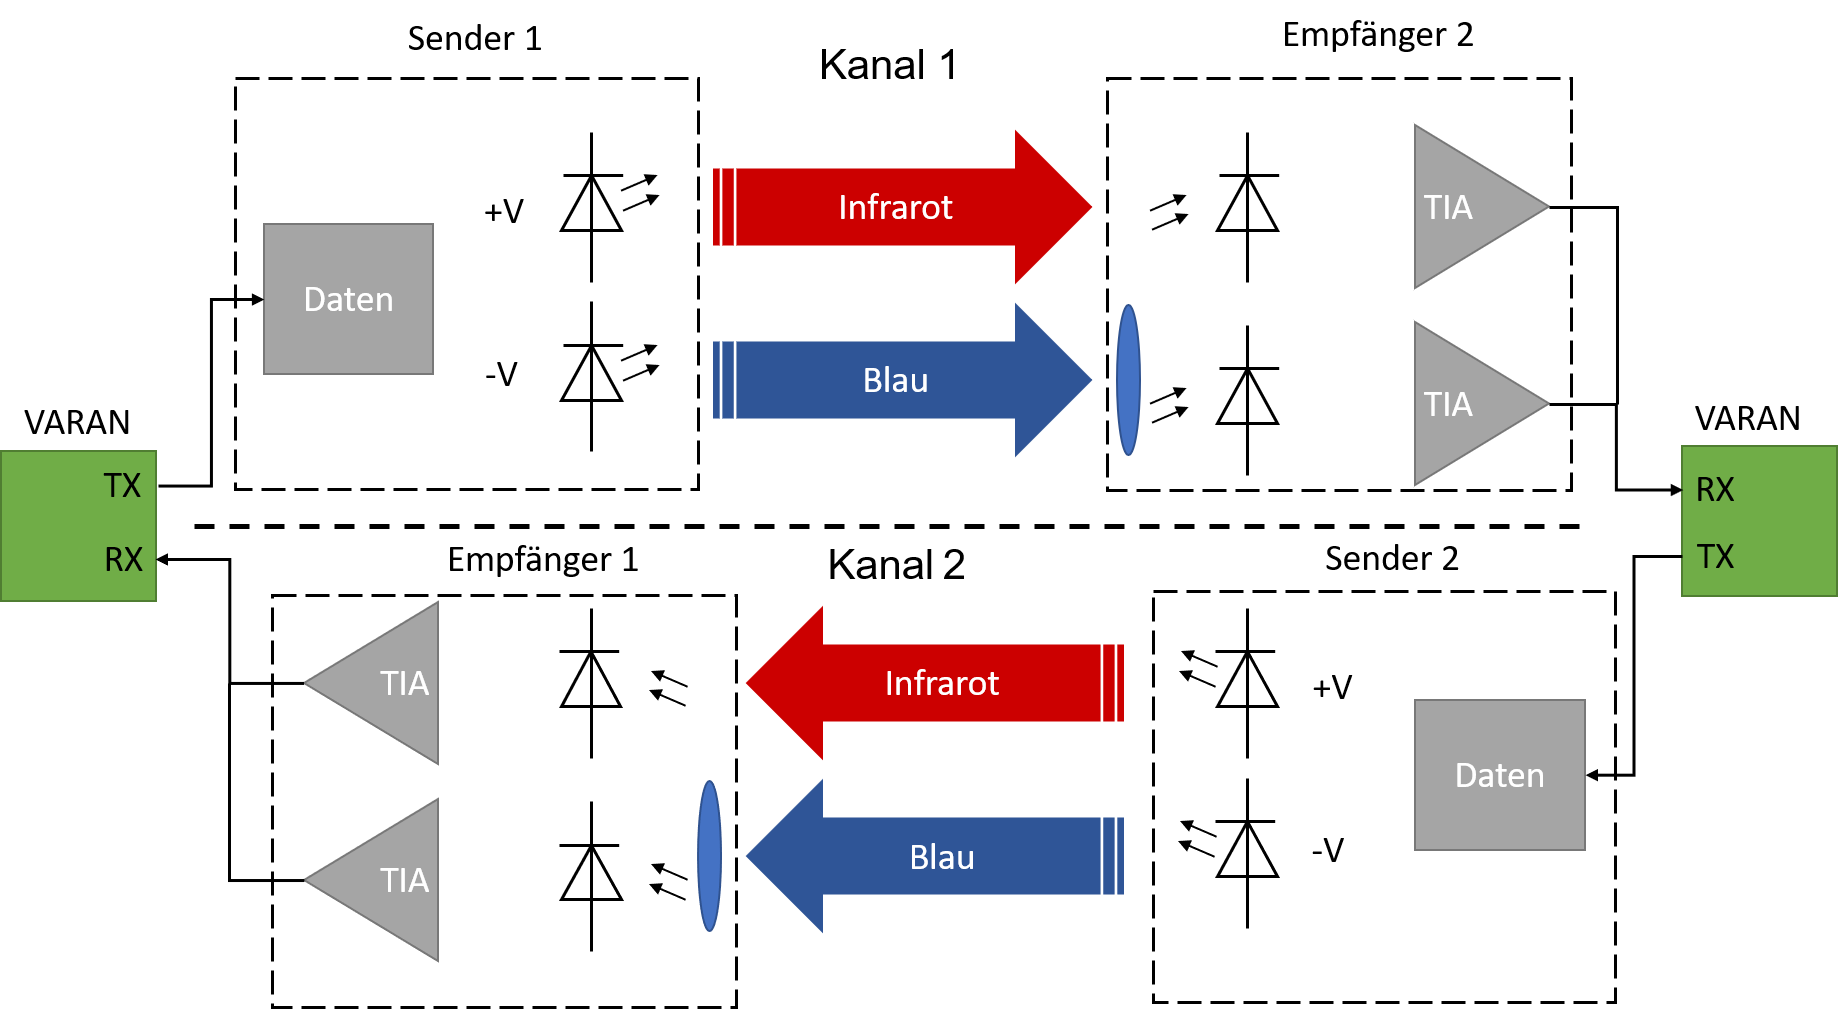
\includegraphics[width=\linewidth]{Konzept_Daten.png}
	\caption{Konzept der optischen Datenübertragung}\label{fig:Konzept_Daten}
\end{figure}

In der Abbildung sind die beiden Kanäle zu erkennen, welche optisch voneinander getrennt sind. Jeder Kanal überträgt dabei die Daten nur in jeweils eine Richtung. Beide Kanäle zusammen sorgen für die gewünschte Bidirektionalität. Auf der Primär- und Sekundärseite hat es jeweils eine Sende- und Empfangseinheit. Eine Sendeeinheit besteht aus der Datenerfassung und den Leuchtdioden. Da der VARAN-Bus MLT-3 codiert ist, müssen drei Zustände übertragen werden können. Die positiven Spannungspegel werden mit einer Infrarot-LED übertragen und die negativen Spannungspegel mit einer blauen LED. Der Zustand \glqq0\grqq steht an, wenn keine der LEDs leuchtet.
\newline
Eine Empfangseinheit besteht aus Photodioden, Verstärkerschaltungen und der Pegelanpassung. Im blauen Spektralbereich werden mit Hilfe eines optischen Filters vor der Photodiode die unerwünschten Spektralanteile herausgefiltert.
\newline Die beiden Sende- und Empfangseinheiten sind identisch aufgebaut und unterscheiden sich nur in der Übertragungsrichtung.

\paragraph{Sender}
In folgender Abbildung ist das Konzept einer Sendeeinheit detaillierter dargestellt.

\begin{figure}[H]
	\centering
	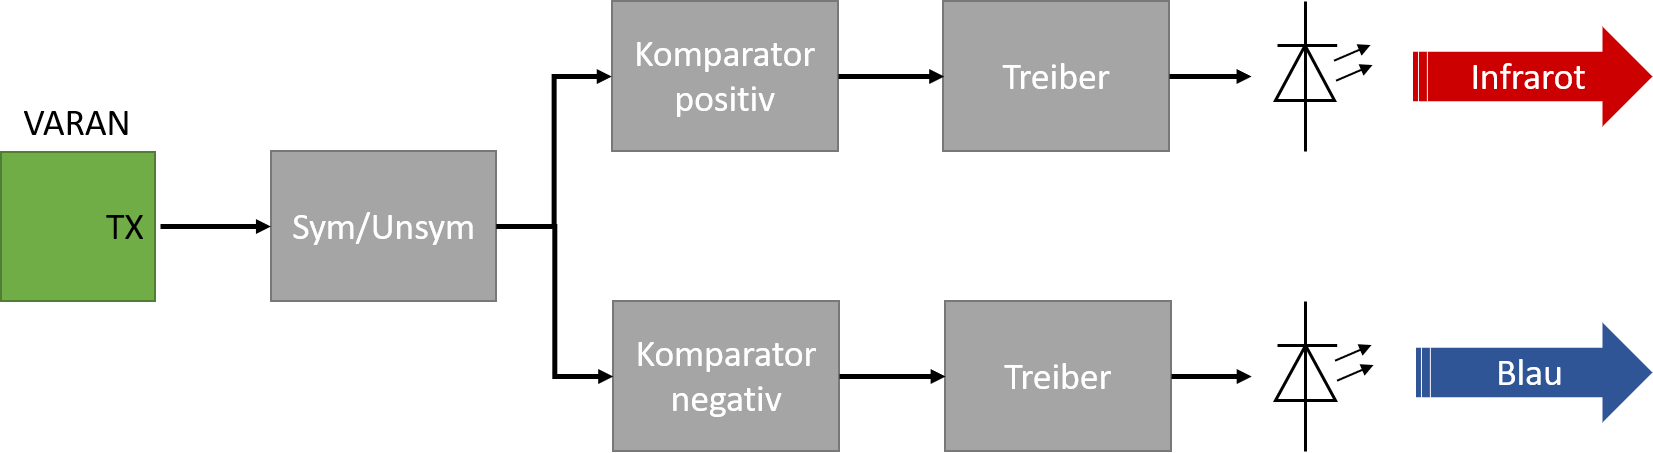
\includegraphics[width=\linewidth]{Konzept_Sender.png}
	\caption{Konzept der optischen Sendeeinheit}\label{fig:Konzept_Sender}
\end{figure}

Aus dem symmetrischen Signal des VARAN-Buses wird zuerst ein unsymmetrisches Signal erzeugt. Dafür kann ein Signal-Transformator eingesetzt werden. Das Signal hat nun einen Bezug zur Masse der restlichen Schaltung. Mit zwei Komparatoren wird unterschieden, ob es sich um einen positiven oder negativen Pegel handelt. Dafür werden Komparatoren mit möglichst kurzer Verzögerungszeit und ausreichender Bandbreite verwendet. Die Komparatoren steuern anschliessend die entsprechenden Treiber an. Als Treiber dient ein FET-Treiber Baustein mit hoher Treiberspannung für schnelle Anstiegs- und Abfallzeiten. Die LED wird mit einem N-Kanal-FET nach Masse geschaltet. Die Schaltzeiten der LED sind entscheidend um auf die geforderte Schaltfrequenz von \textgreater \SI{30}{MHz} zu kommen. Dafür wurde einerseits ein FET mit kleiner Gate-Kapazität gewählt und andererseits auf kurze Anstiegs- und Abfallzeiten der LED geachtet.
\newline
Mit einer kleinen Erweiterung der Beschaltung der LED können die Anstiegs- und Abfallzeiten nochmals reduziert werden. Folgende Abbildung zeigt die Ansteuerung der LED mitsamt der Erweiterung von $R_{2}$, $C$ und $L$.

 \begin{figure}[h]
 	\centering
 	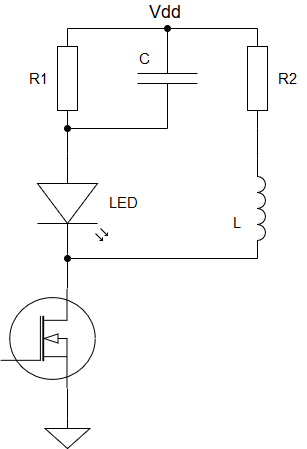
\includegraphics[width=0.3\linewidth]{Fast_LED.png}
 	\caption{Erweiterte Schaltung um Schaltzeiten zu verkürzen}\label{fig:Fast_LED}
 \end{figure}

Durch den Leckstrom des FET wird die LED auch im abgeschalteten Zustand mit einigen Ladungsträgern durchflossen, was die Anstiegszeit geringfügig verkürzt. Im Einschaltmoment sorgt der Kondensator $C$ für einen Kurzschluss und überbrückt den Vorwiderstand $R_{1}$. Es kommt zu einem Strompeak, der die Kapazität der LED schneller laden lässt. Die Anstiegszeit wird dadurch massiv verkürzt. Im Ausschaltmoment induziert das Magnetfeld in der Spule $L$ eine negative Spannung. Folglich werden die Ladungsträger aus der LED gezogen. Dadurch wird auch die Abfallzeit gegenüber dem \glqq einfachen\grqq Ausschalten verkürzt.

\paragraph{Empfänger}
In folgender Abbildung wird das Konzept einer Empfangseinheit detaillierter dargestellt.

\begin{figure}[h]
	\centering
	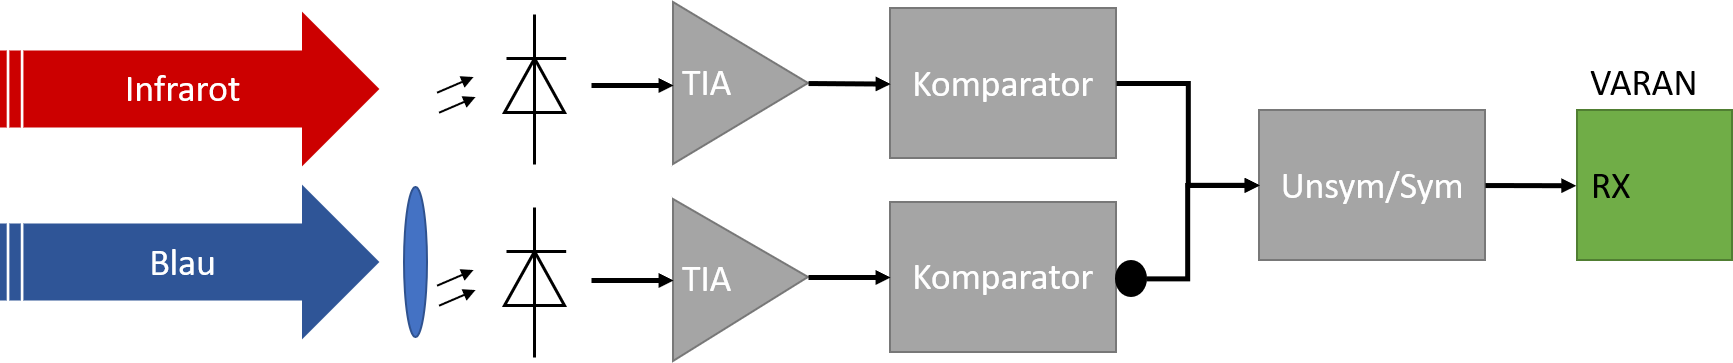
\includegraphics[width=\linewidth]{Konzept_Empfaenger.png}
	\caption{Konzept der optischen Empfangseinheit}\label{fig:Konzept_Empfaenger}
\end{figure}

Der von der Photodiode erzeugte Strom wird mit einer Transimpedanzverstärkerschaltung in eine Spannung gewandelt und verstärkt. Wie im Kapitel \nameref{sec:Grundlagen} bereits erwähnt, ist eine hohe Bandbreite bei der Verstärkerschaltung erforderlich. Deshalb ist ein Verstärker mit hohem Gain-Bandwidth Product und kleiner Eingangskapazität zu wählen. Auch die parasitäre Kapazität der Photodiode beeinflusst die Bandbreite, weshalb auch diese möglichst klein gewählt werden muss. Durch negative Biasspannung an der Anode kann die Kapazität nochmals reduziert werden.
\newline
Nach dem Transimpedanzverstärker werden mit Komparatoren die Pegel in Amplitude und Form angepasst. Das Signal vom blauen Spektralbereich, welches die negativen Pegel überträgt wird noch invertiert. Mit einem Signal-Transformator wird aus dem unsymmetrischen Signal wieder ein symmetrisches Signal generiert und dieses zurück an den VARAN-Bus geführt.

\paragraph{Kanal}
Da die optische Übertragung auf einer drehbaren Konstruktion stattfindet, ist keine direkte Verbindung sichergestellt. Deshalb bestehen die beiden Kanäle aus einem lichtstreuenden Werkstoff und sind optisch voneinander isoliert. Nachfolgende Abbildung zeigt den prinzipiellen Aufbau der Kanäle.

\begin{figure}[h]
	\centering
	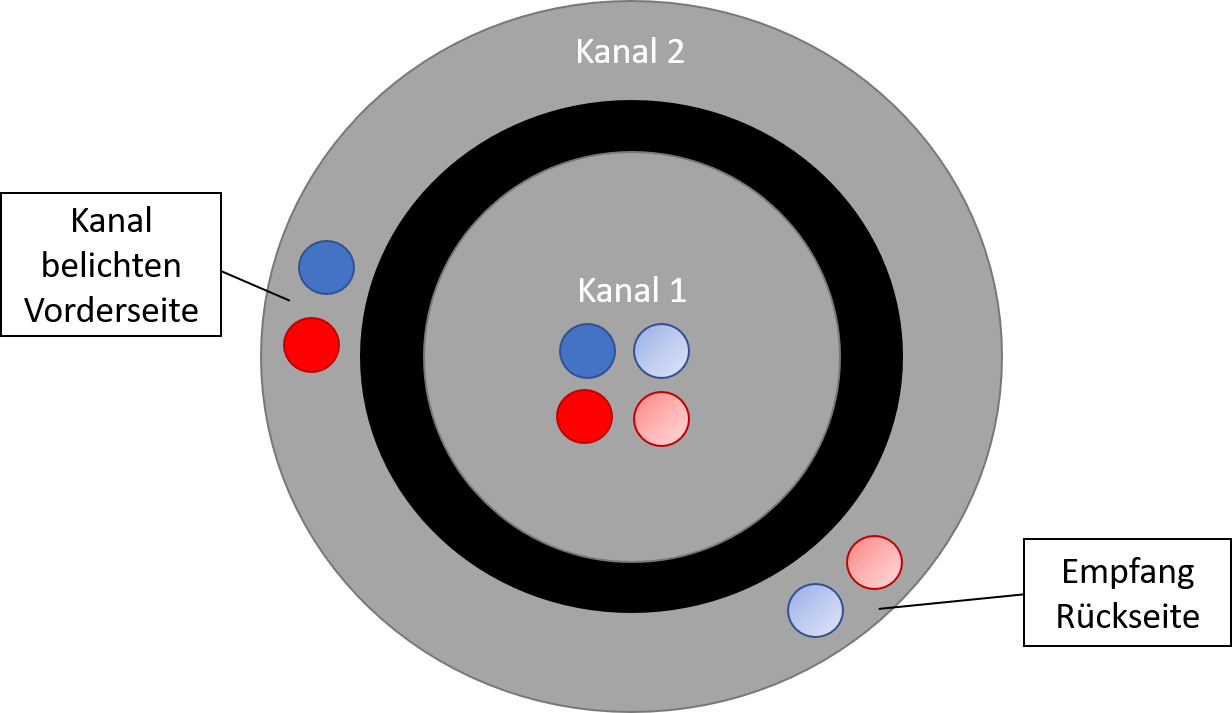
\includegraphics[width=0.6\linewidth]{Konzept_Kanal.png}
	\caption{Konzept der Kanäle}\label{fig:Konzept_Kanal}
\end{figure}

In der Abbildung ist die optische Isolation (schwarz) gut zu erkennen, welche die gegenseitige Beeinflussung der beiden Kanäle verhindert. Im Kanal 1 ist die Rotation der mechanischen Konstruktion unproblematisch, da sich Sender und Empfänger auf der Drehachse befinden. Der Kanal 2 nimmt das Licht auf der einen Seite auf und der lichtstreuende Werkstoff (grau) verteilt es im ganzen Kreisring. Nun spielt es auf der Empfängerseite keine Rolle mehr, in welchem Abschnitt auf dem Kreisring man sich befindet.

\subsection{Dimensionierung Testaufbau}
Um wichtige Erkenntnisse für den weiteren Projektverlauf zu gewinnen, wurde ein Testaufbau realisiert. Dieser beinhaltet eine Sende- und Empfangseinheit um ein Rechtecksignal im Infrarotbereich zu übertragen. 
In diesem Unterkapitel wird auf die wichtigsten Punkte zur Dimensionierung des Testaufbaus eingegangen. Das entsprechende Schema mit der Detailbeschaltung ist dem Anhang zu entnehmen.
\paragraph{Sender} 
Als Eingang beim Sender dient eine BNC-Buchse, um das Rechtecksignal einzuspeisen. Als Gatetreiber des FET wird der ISL55110 vom Hersteller Renesas verwendet. Dieser zeichnet sich durch kurze Anstiegs- und Fallzeiten von \SI{1.5}{ns} bei einer Last von \SI{100}{pF} aus.
Der gewählte N-Kanal-FET ist ein BSS316N vom Hersteller Infineon. Durch die kleine Eingangskapazität von \textless \SI{100}{pF} kann der FET in Kombination mit dem Gatetreiber sehr schnell geschaltet werden.
Als Infrarot-Emitter wurde die SFH4235 von OSRAM gewählt. Die Leuchtdiode kann mit Anstiegs- und Abfallzeiten von 7/\SI{14}{ns} mit \textgreater \SI{30}{MHz} betrieben werden und ist deshalb für diese Anwendung geeignet. Folgende Abbildung zeigt das Spektrum des Infrarot-Emitters.

\begin{figure}[h]
	\centering
	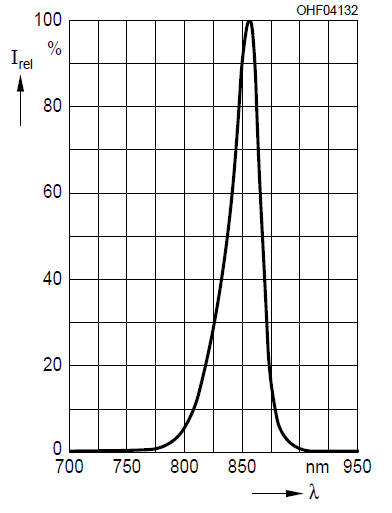
\includegraphics[width=0.4\linewidth]{Spektrum_Infra.png}
	\caption{Spektrum SFH4235}\label{fig:Spektrum_Infra}
\end{figure}

Wie in der Abbildung zu erkennen ist, hat das Spektrum den Peak bei \SI{860}{nm}. Die Photodiode auf der Empfängerseite muss dementsprechend passend zum Spektrum ausgewählt werden. Die im Konzept beschriebene Schaltungsergänzung wurde im Testaufbau vorbereitet. Weil die einfache Ansteuerung schnell genug ist, wird die Ergänzung vorerst nicht bestückt.

\paragraph{Empfänger}
Mit zwei Z-Dioden (SZBZX84C3V3 und BZD27C13) und einem Operationsverstärker (LM7321) als Buffer geschaltet, wird eine Speisung für die Empfängerschaltung generiert. Diese liefert die benötigten Spannungen von \SI{3.3}{V} für die integrierten Bauteile und \SI{-13}{V} um die Photodiode mit einer negativen Biasspannung vorzuspannen. Die Beschaltung ist im Schema im Anhang abgebildet.
\newline
Es wurden drei verschiedene Photodioden ausgewählt und analysiert.

\begin{table}[H]
\begin{tabular}{|l|l|l|l|}
	\hline 
	\textbf{Typ}&\textbf{$C_{p} (V_{R}=\SI{0}{V})$}  & \textbf{$C_{p} (V_{R}=\SI{-13}{V})$} & \textbf{Wellenlänge max. Sensitivität} \\ 
	\hline 
	SFH 203 FA Osram&\SI{11}{pF}  & \SI{2.5}{pF} & \SI{900}{nm} \\ 
	\hline 
	SFH 2701 Osram&\SI{3}{pF}  &\SI{1.7}{pF}  &\SI{820}{nm}  \\ 
	\hline 
	S5972 Hamamatsu&\SI{6}{pF}  &\SI{2.8}{pF}  &\SI{800}{nm}  \\ 
	\hline 
\end{tabular} 
\caption{Datenblattwerte der ausgewählten Photodioden}\label{tab:Tabelle_Photo}
\end{table}

Wie aus der Tabelle zu entnehmen ist, kann die parasitäre Kapazität aller ausgewählten Photodioden durch die negative Biasspannung auf einen Wert \textless \SI{3}{pF} gebracht werden. Dieser Wert dient als Ausgangslage für weitere Berechnungen und Simulationen.
\newline
Um einen Anhaltspunkt für den zu erwartenden Photostrom zu haben, wurden die Photodioden bei Bestrahlung mit dem Infrarot-Emitter ($I_{F}=\SI{280}{mA}$, konstant) ausgemessen.


\begin{tikzpicture}
\begin{axis}[
title={Photostrom in Abhängigkeit des Abstandes},
xlabel={Abstand [cm]},
ylabel={Photostrom [$\mu$ A]},
xmin=0, xmax=10,
ymin=0, ymax=1500,
ymode=log,
xtick={0,2,4,6,8,10},
%ytick={0,5,10,50,100,500,1000},
legend pos=north east,
ymajorgrids=true,
yminorgrids=true,
grid style=dashed,
]

\addplot[
color=blue,
mark=square,
]
coordinates {
	(0.5,300)(1,137)(1.5,82)(2,55)(2.5,32)(3,24)(3.5,19)(4,15)(4.5,12)(5,9)(7,5)(9,3.2)(10,2.6)
};

\addplot[
color=red,
mark=square,
]
coordinates {
	(0.5,1500)(1,1050)(1.5,650)(2,460)(2.5,340)(3,250)(3.5,200)(4,165)(4.5,138)(5,115)(7,63)(9,42)(10,32)
};

\addplot[
color=green,
mark=square,
]
coordinates {
	(0.5,400)(1,210)(1.5,90)(2,50)(2.5,30)(3,24)(3.5,17)(4,14)(4.5,11)(5,9)(7,4.5)(9,2.8)(10,2.2)
};
\legend{S5972,SFH203,SFH2701}

\end{axis}
\end{tikzpicture}

Aus der Grafik geht hervor, dass bei einer Distanz von \SI{4}{cm} mit einem Photostrom von \textgreater $\SI{10}{\mu A}$ gerechnet werden kann. Diese Distanz wurde abgeschätzt und hängt von der späteren mechanischen Konstruktion ab. Sie dürfte aber eher kleiner werden, weshalb diese Annahme getroffen wurde.
\newline
Als Transimpedanzverstärker wurde der LT6268 von Linear Technology gewählt. Dieser Verstärker ist durch sein hohes GBWP von \SI{4}{GHz} und der kleinen Eingangskapazität von \SI{0.45}{pF} für High-Speed Photoanwendungen geeignet.

Gemäss Formel \ref{eq:Bandwidth} ist mit diesem Verstärker in Kombination mit einer der ausgewählten Photodioden folgende Bandbreite möglich:

\begin{equation}\label{eq:Bandwidth2}
B=\sqrt{\frac{GBWP}{2\pi\cdot R_{f}\cdot (C_{opamp}+C_{photo})}}\approx \SI{96}{MHZ}
\end{equation}

Dabei wurde mit $R_{f}=\SI{20}{k\omega}$, $GBWP=\SI{4}{GHz}$, $C_{opamp}=\SI{0.45}{pF}$ und $C_{photo}=\SI{3}{pF}$ gerechnet.

Gemäss Datenblatt des Verstärkers braucht es eine Kapazität im Feedback-Loop für eine stabile Funktionalität im höheren Frequenzbereich. Dafür gelten folgende Bedingungen:
\begin{equation}\label{eq:Amp_Cf}
C{f}\textgreater \sqrt{\frac{C_{IN}}{\pi\cdot GBWP\cdot R_{f}}}
\end{equation}

\begin{equation}\label{eq:Cin_Cf}
\frac{C_{IN}}{C_{f}}\geq 10
\end{equation}

Mit den beiden Formeln \ref{eq:Amp_Cf} und \ref{eq:Cin_Cf} bekommt man folgende Bedingung für $C_{f}$: 
\begin{equation}\label{eq:Cfminmax}
\SI{150}{fF}\textgreater C_{f}\textgreater \SI{500}{fF}
\end{equation}

\todo[inline]{ Unterkapitel noch abschliessen und zur Simulation überleiten}

\subsection{Simulation}
Im Simulations-Abschnitt wird die Dimensionierung und das Konzept überprüft.
\subsection{Testaufbau}
In diesem Unterkapitel wird der Testaufbau beschrieben.
\section{Fazit}
\label{sec:Fazit}

In diesem Kapitel wird das Erreichte beschrieben. Es wird erklärt, welche Schlüsse gezogen wurden und mit welcher Ausgangslage das Projekt 6 gestartet werden könnte.

\todo[inline]{Simulation und Realität sehr nahe}

%%---BIBLIOGRAPHY------------------------------------------------------------------------
{\sloppypar
\printbibliography[heading=bibintoc]
\label{sec:lit}
}

%%---APPENDIX----------------------------------------------------------------------------
\begin{appendix} %Anhang

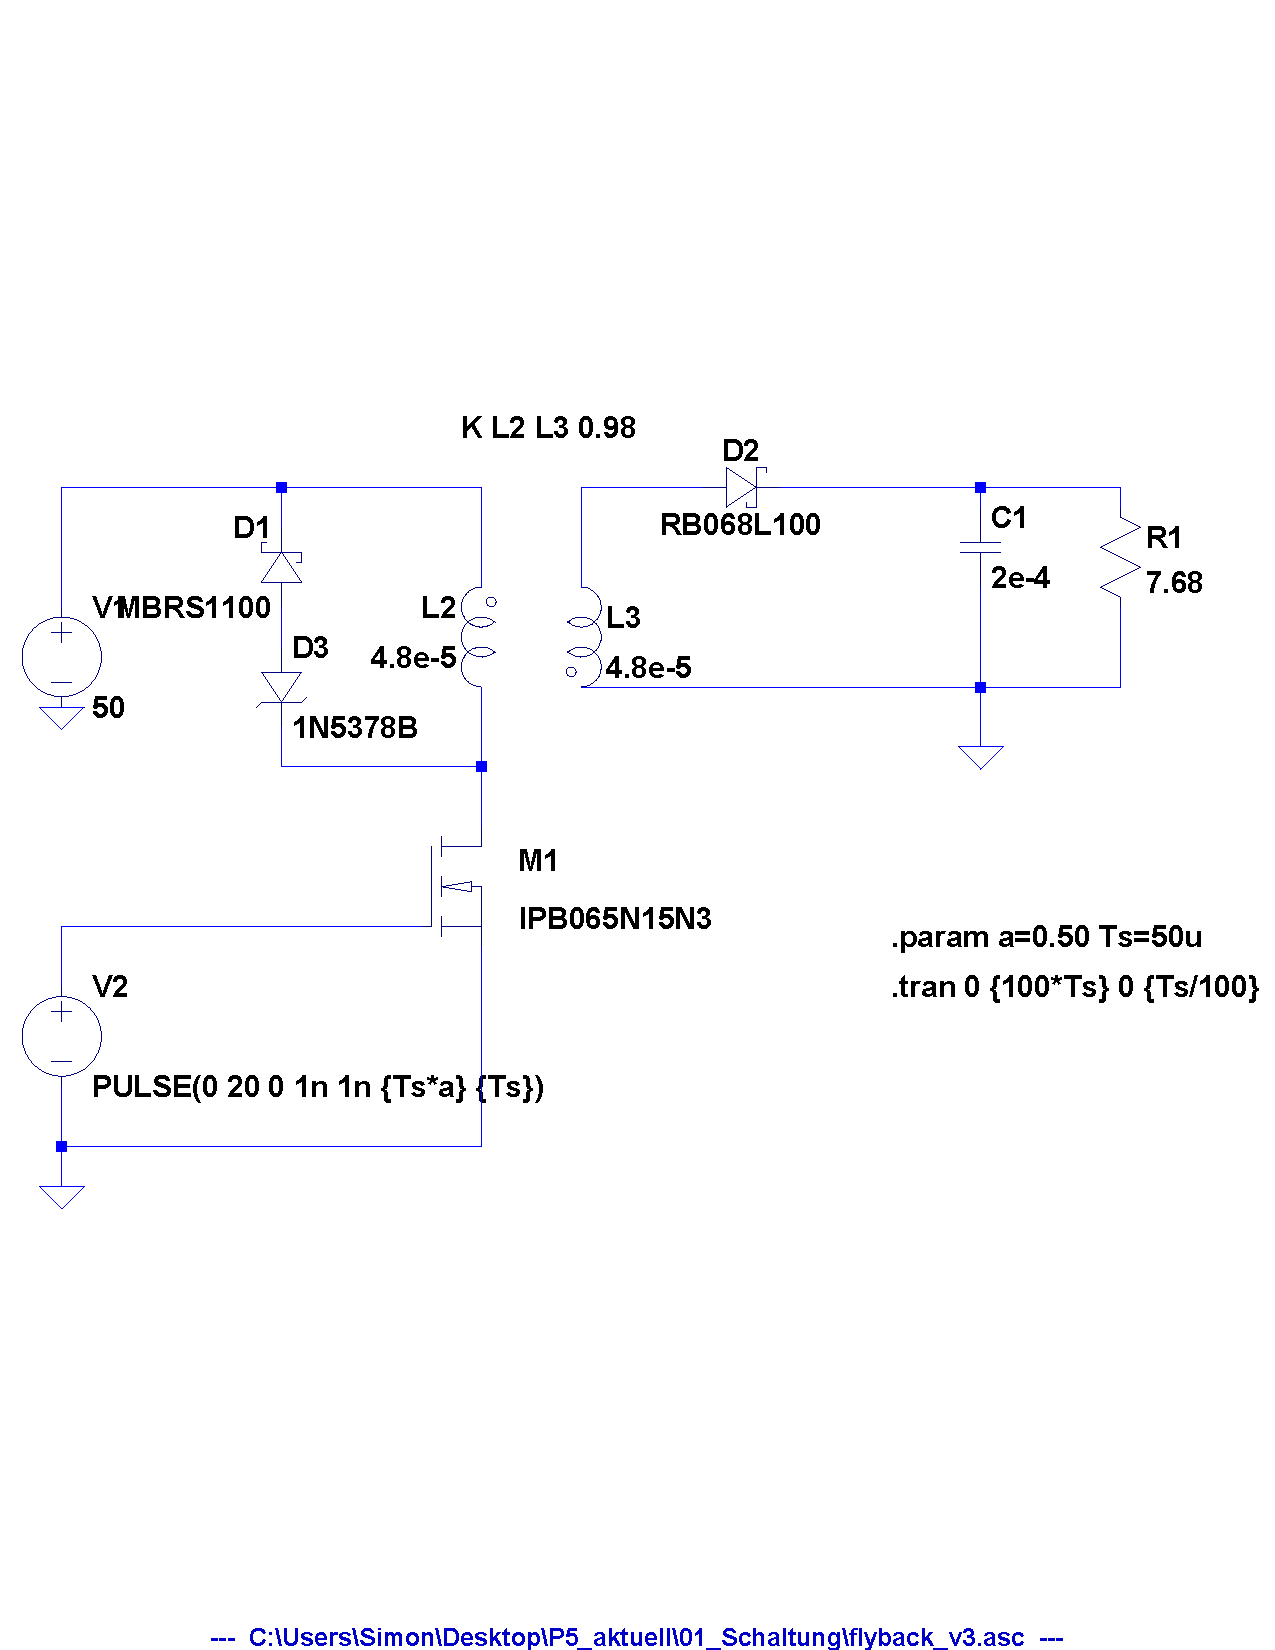
\includepdf[pages={1},nup=1x1,landscape=true,scale=0.85,offset=10 -40,pagecommand={\section{Simulation LTSpice Flyback-Converter}\label{app:Sim_LTSpice_Energie}\thispagestyle{myheadings}}]{appendix/Sim_LTSpice_energie.pdf} \newpage

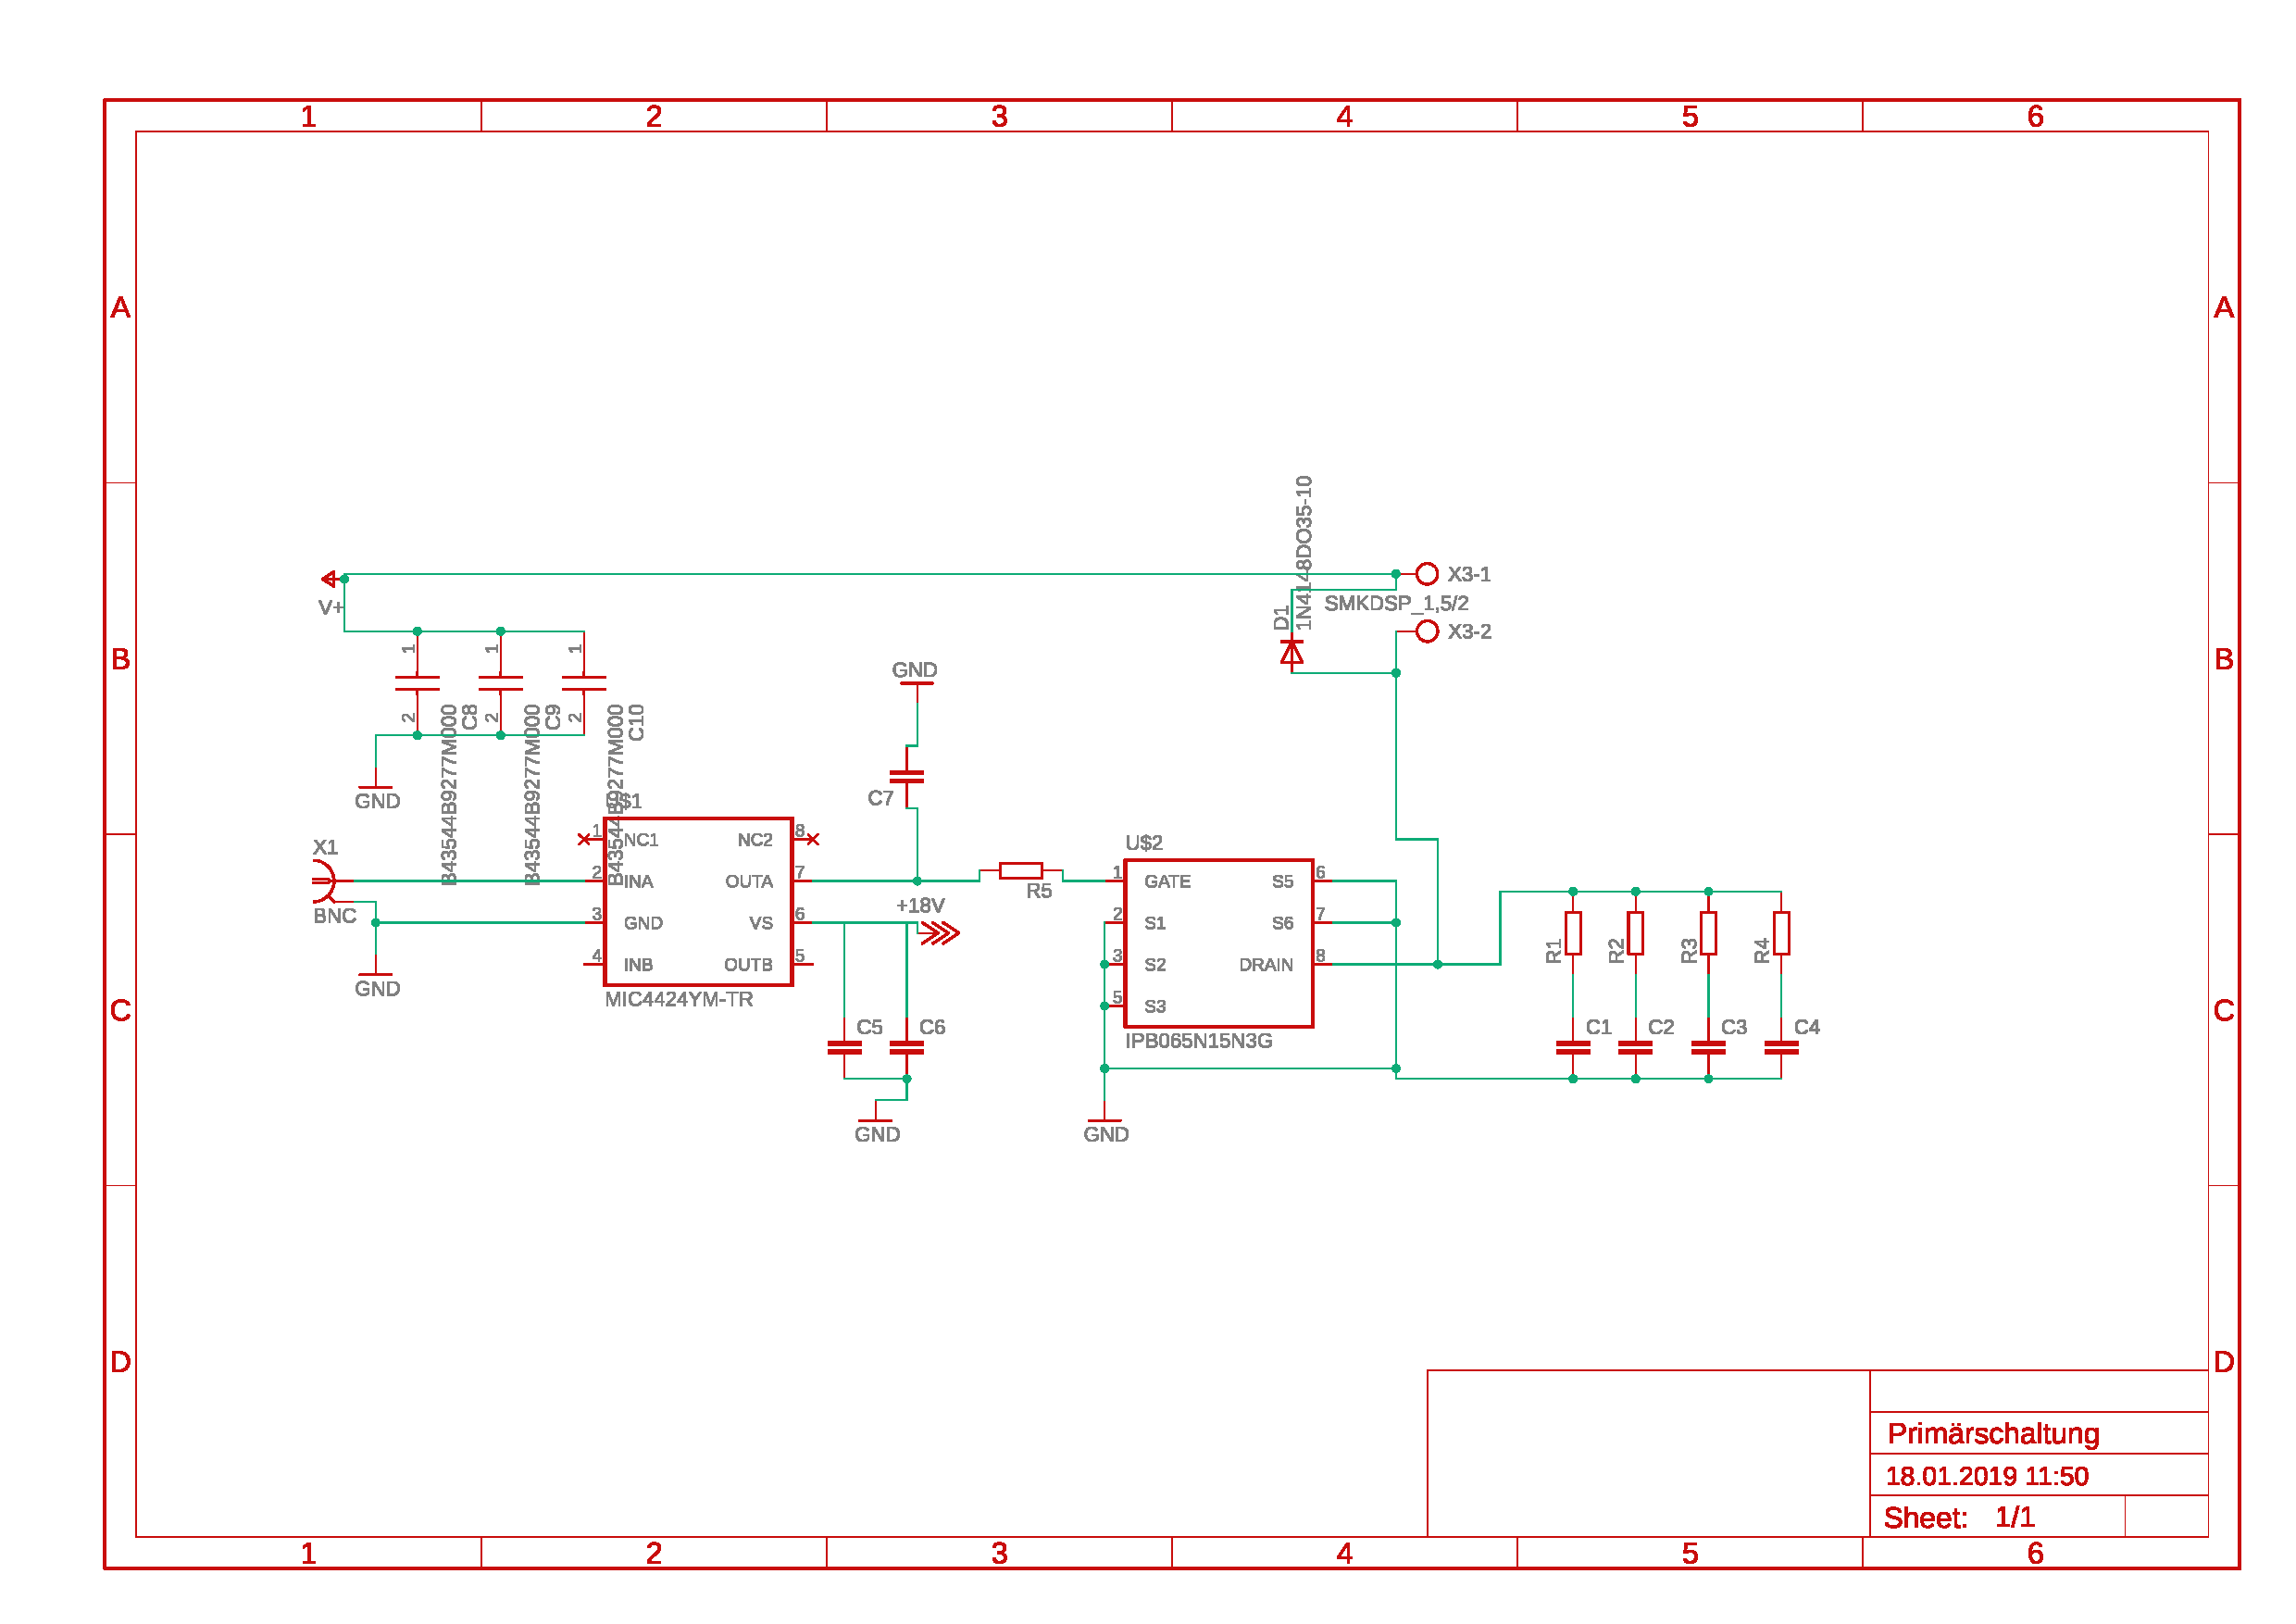
\includepdf[pages={1},fitpaper,nup=1x1,landscape=true,scale=0.85,offset=10 -40,pagecommand={\section{Schema Primärseite}\label{app:Schema_Primaer}\thispagestyle{myheadings}}]{appendix/schema_primaerschaltung.pdf} \newpage

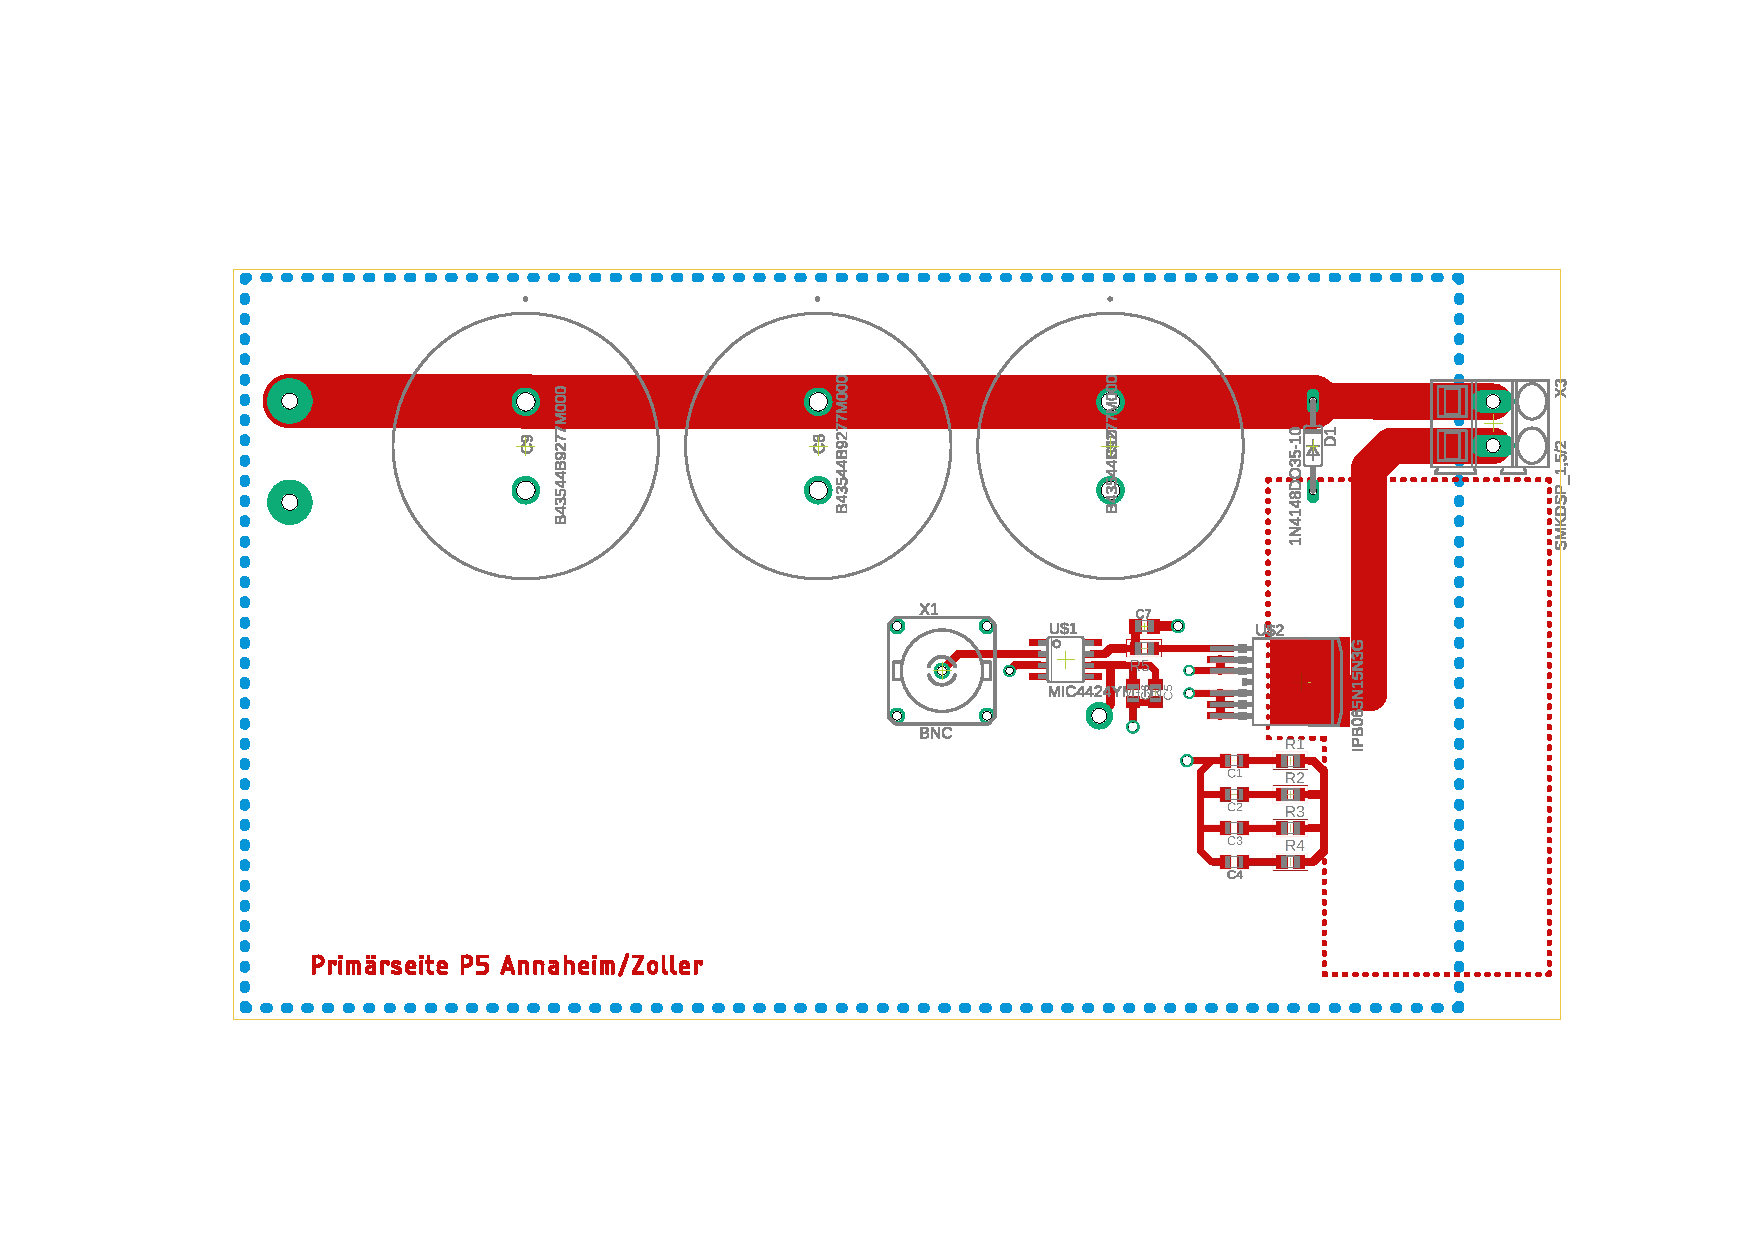
\includepdf[pages={1},nup=1x1,landscape=true,scale=0.85,offset=10 -40,pagecommand={\section{Layout Primärseite}\label{app:Layout_Primaer}\thispagestyle{myheadings}}]{appendix/layout_primaer.pdf} \newpage

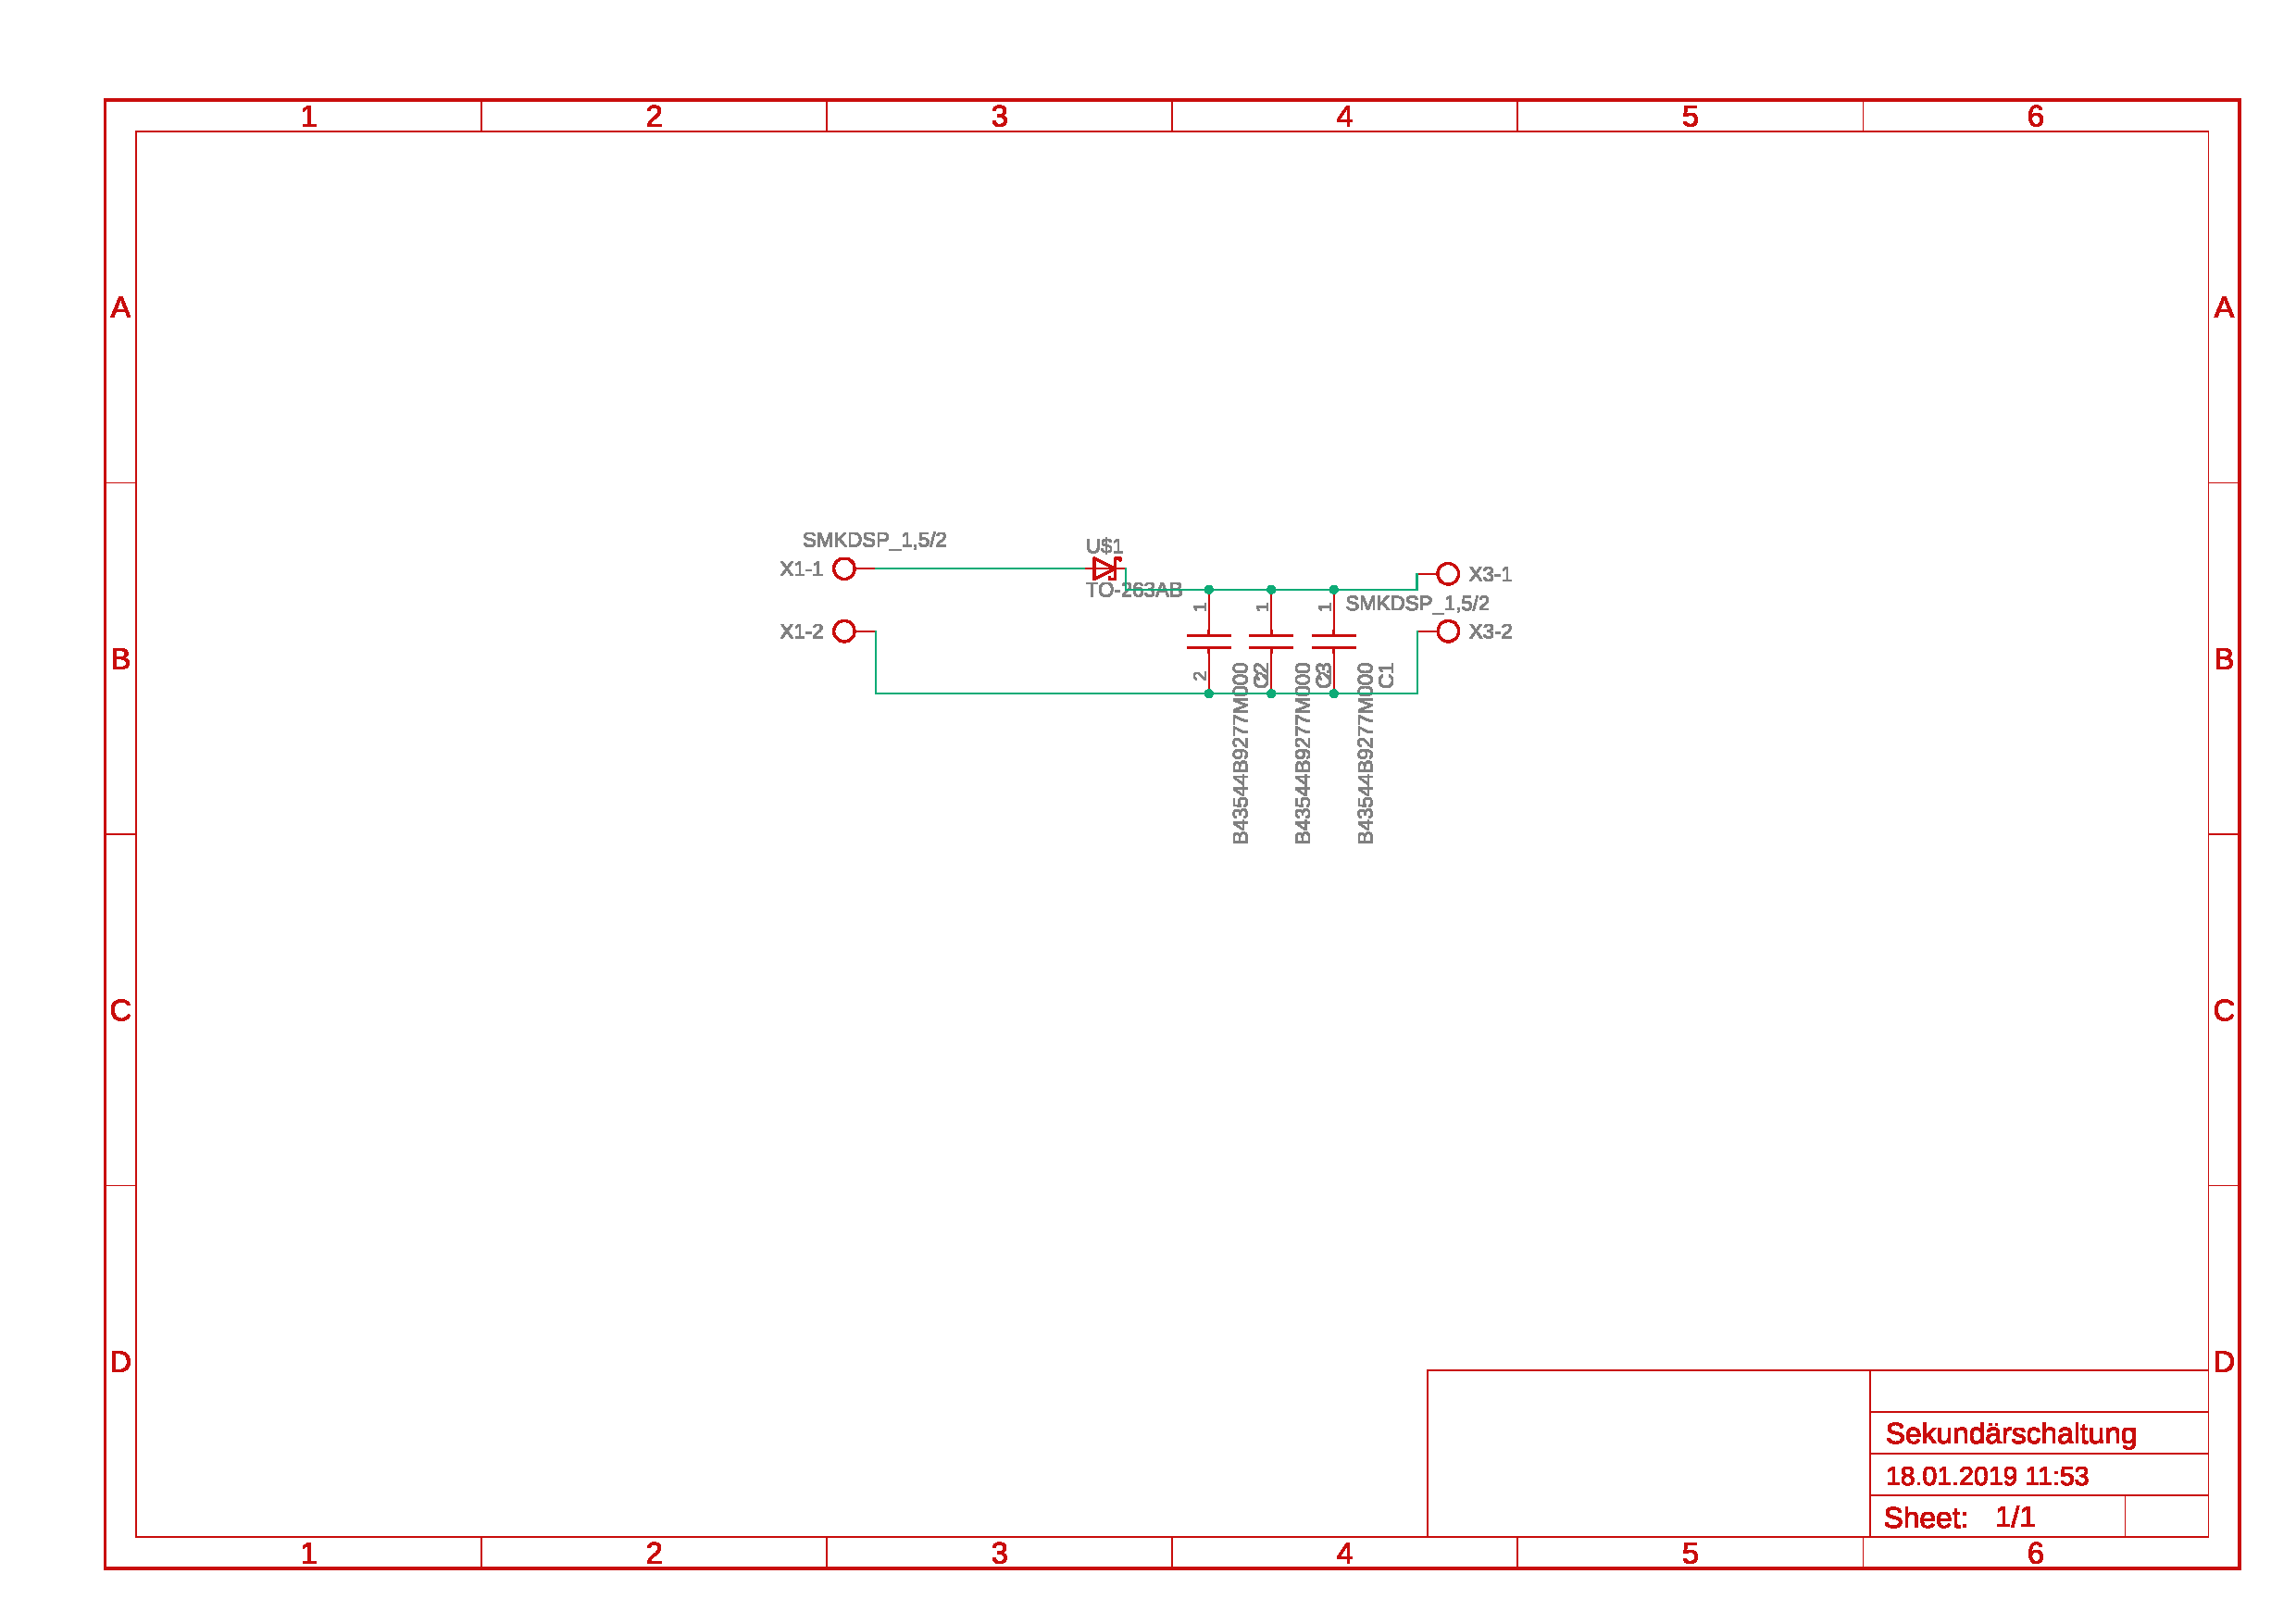
\includepdf[pages={1},fitpaper,nup=1x1,landscape=true,scale=0.85,offset=10 -40,pagecommand={\section{Schema Sekundärseite}\label{app:Schema_Sekundaer}\thispagestyle{myheadings}}]{appendix/schema_sek.pdf} \newpage

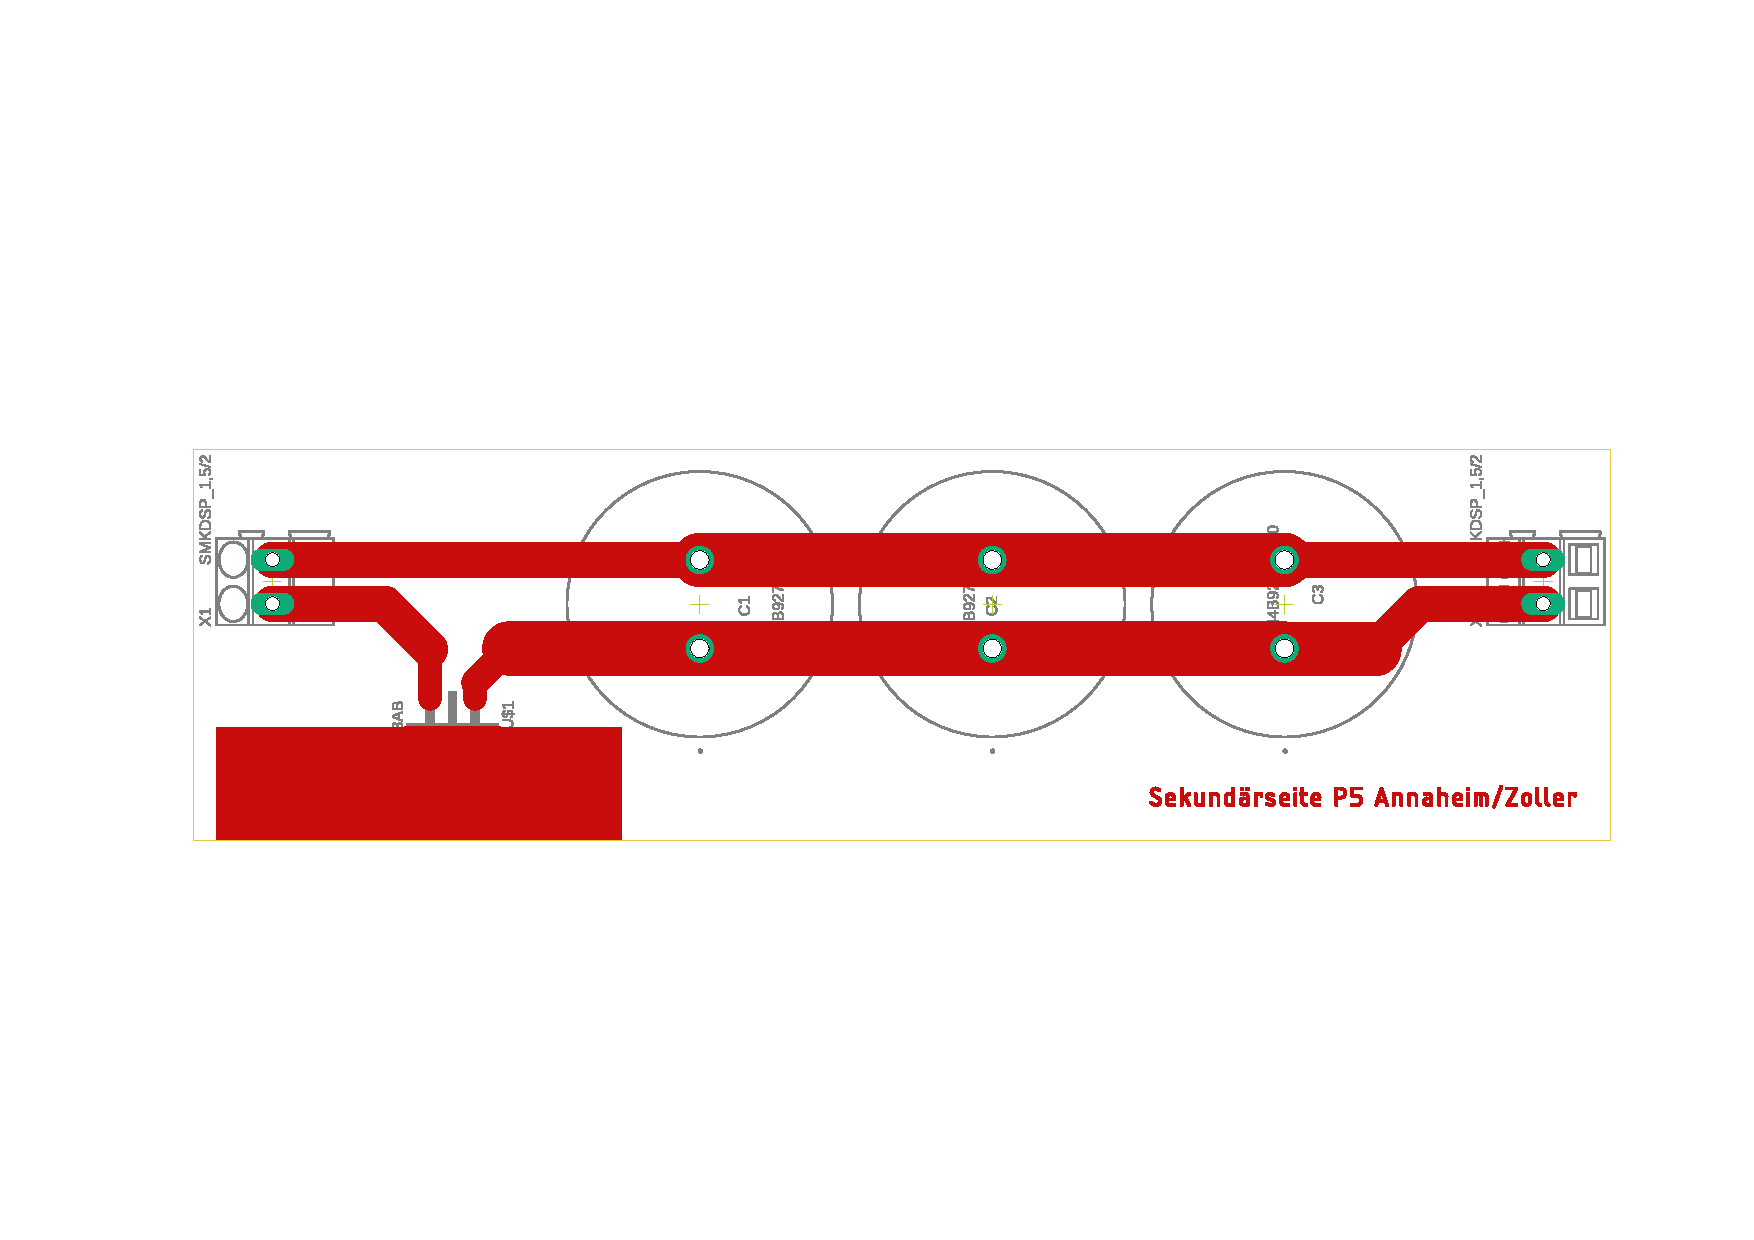
\includepdf[pages={1},nup=1x1,landscape=true,scale=0.85,offset=10 -40,pagecommand={\section{Layout Sekundärseite}\label{app:Layout_Sekundaer}\thispagestyle{myheadings}}]{appendix/layout_sek.pdf} \newpage
	
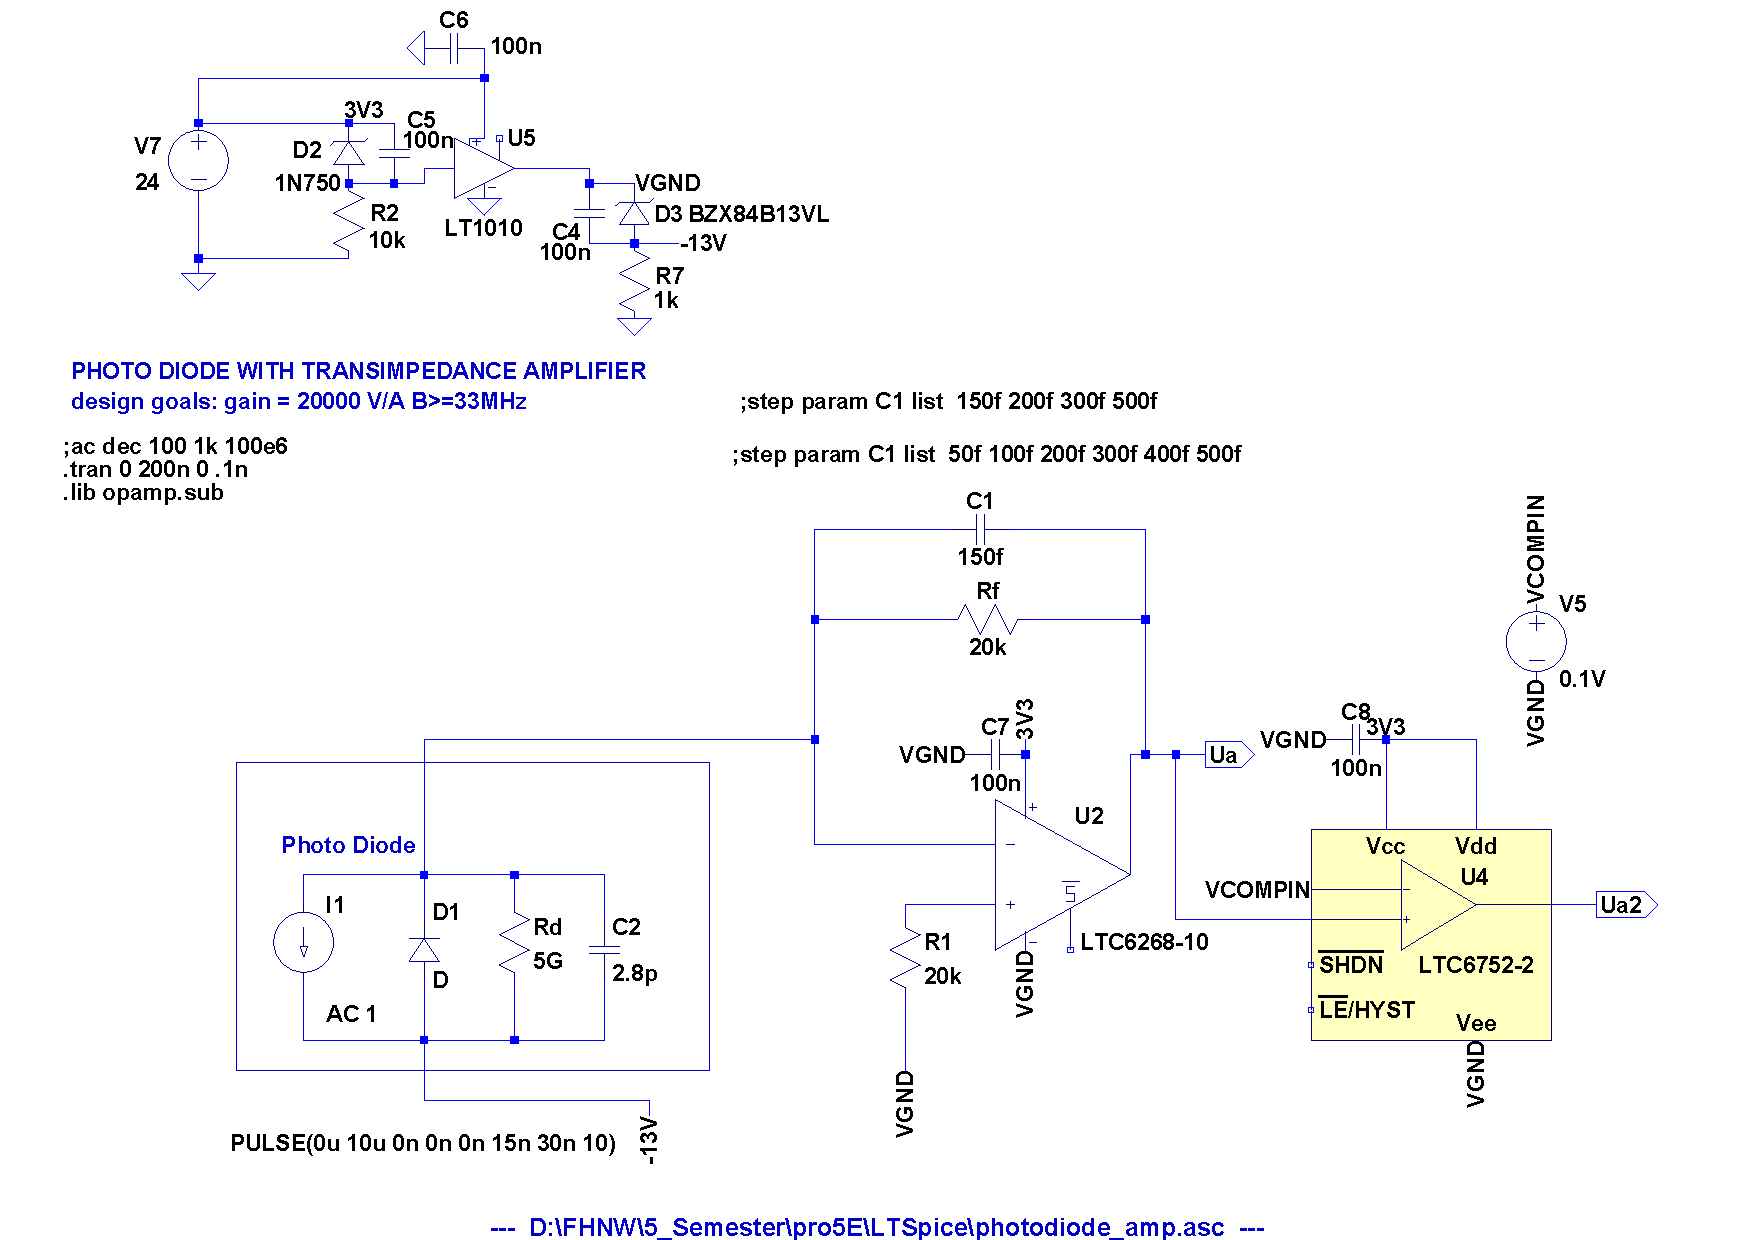
\includepdf[pages={1},nup=1x1,landscape=true,scale=0.85,offset=10 -40,pagecommand={\section{Simulation LTSpice Empfängerschaltung}\label{app:Sim_LTSpice_Data}\thispagestyle{myheadings}}]{appendix/Sim_LTSpice_Data.pdf} \newpage
	
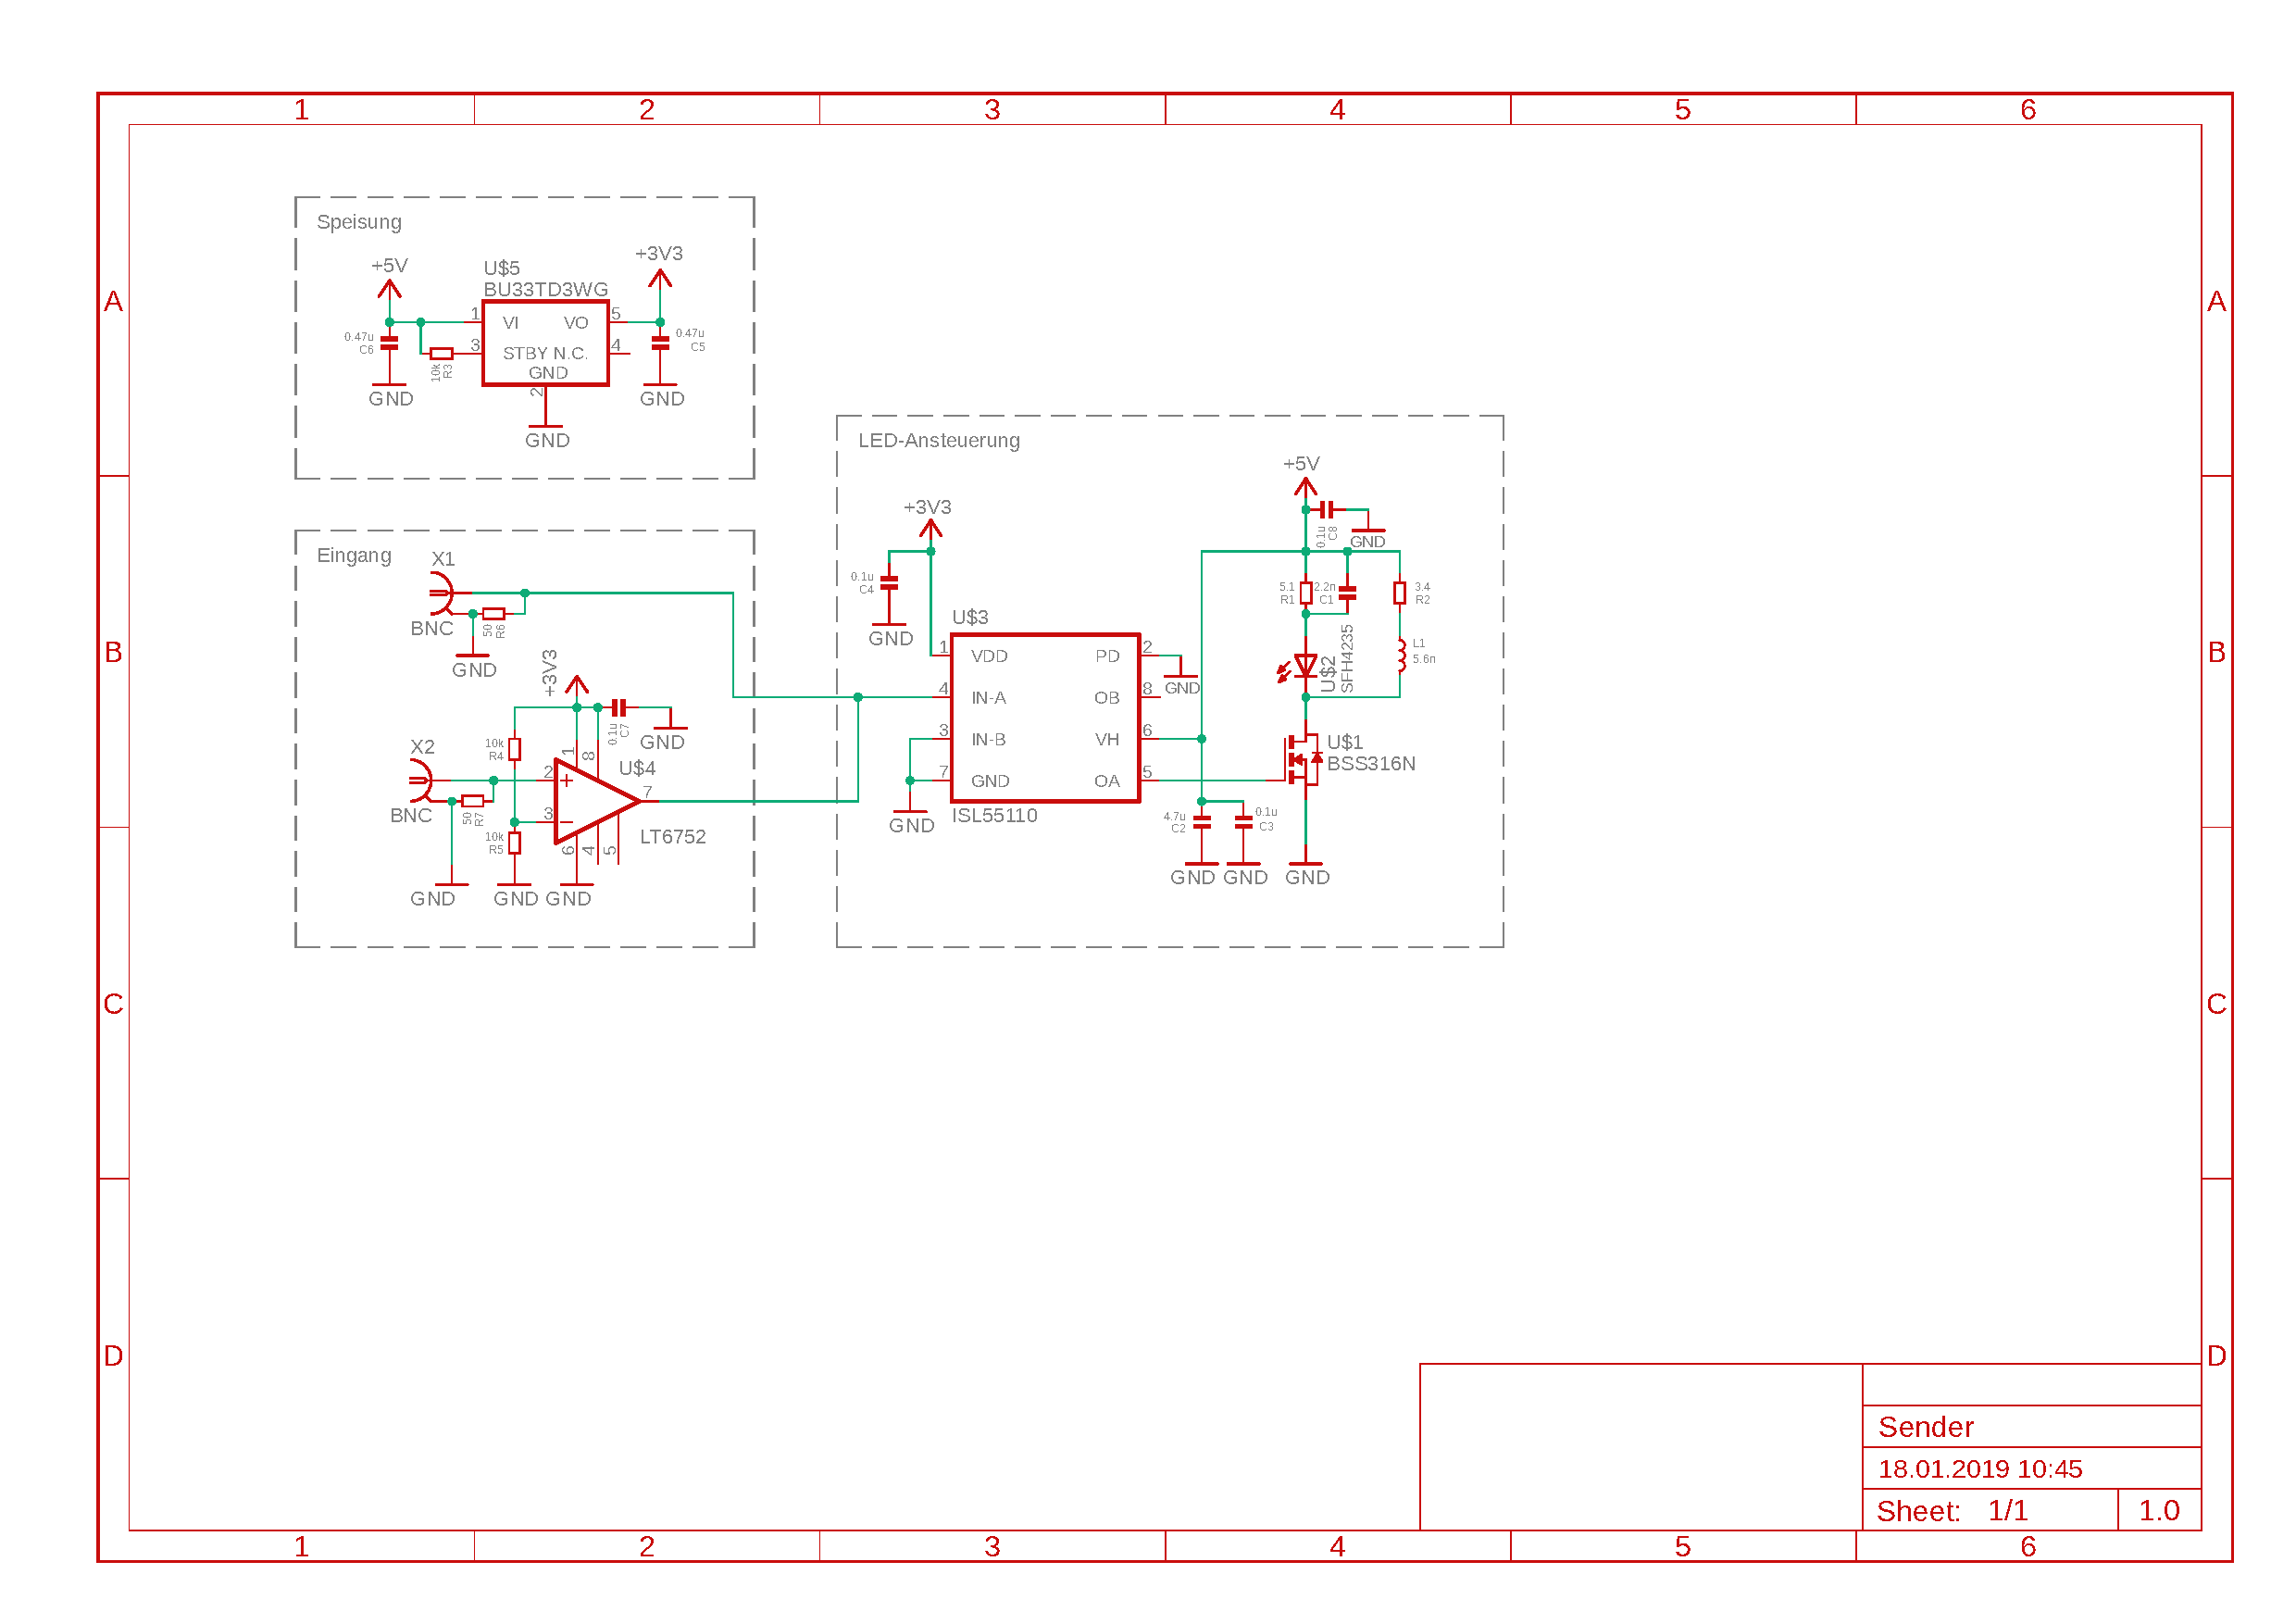
\includepdf[pages={1},fitpaper,nup=1x1,landscape=true,scale=0.85,offset=10 -40,pagecommand={\section{Schema Sender}\label{app:Schema_Sender}\thispagestyle{myheadings}}]{appendix/Schema_Sender.pdf} \newpage

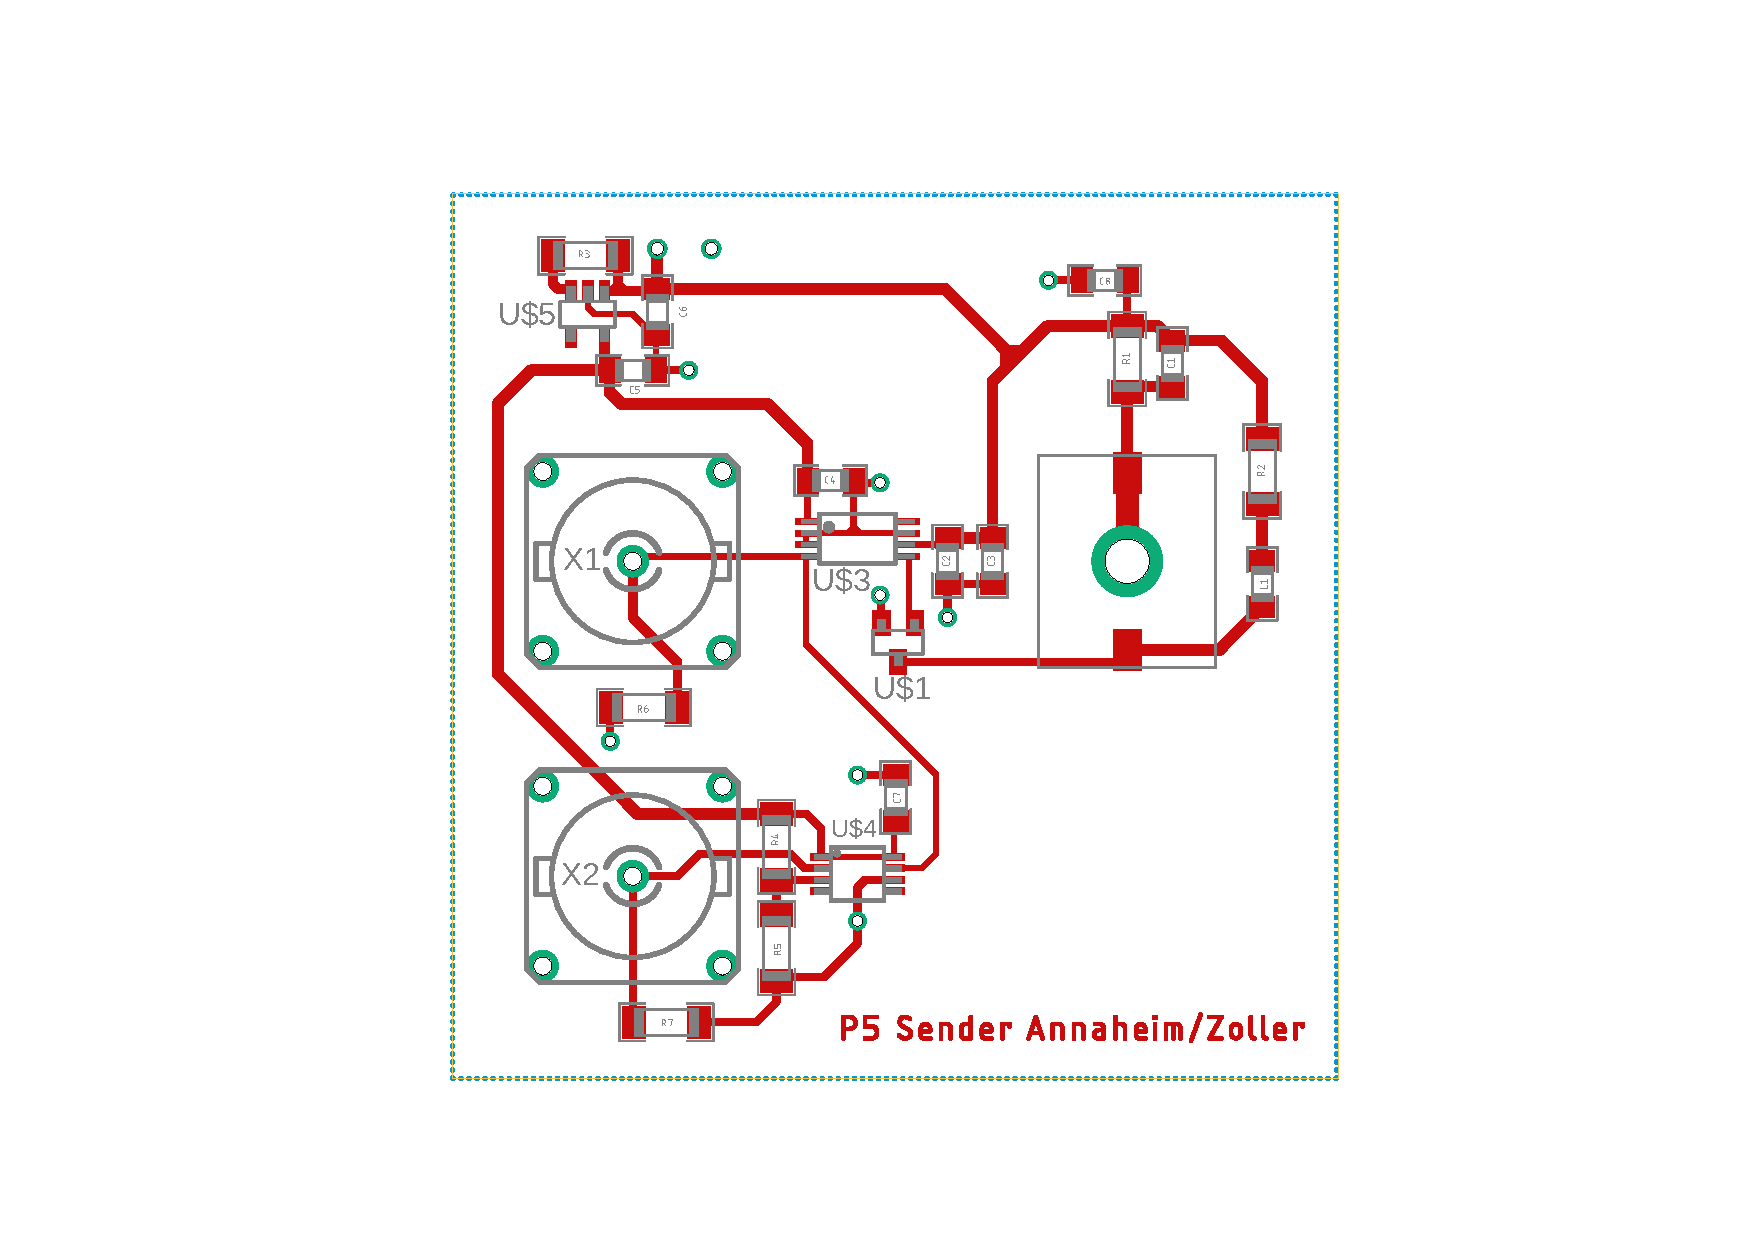
\includepdf[pages={1},nup=1x1,landscape=true,scale=0.85,offset=10 -40,pagecommand={\section{Layout Sender}\label{app:Layout_Sender}\thispagestyle{myheadings}}]{appendix/Layout_Sender.pdf} \newpage

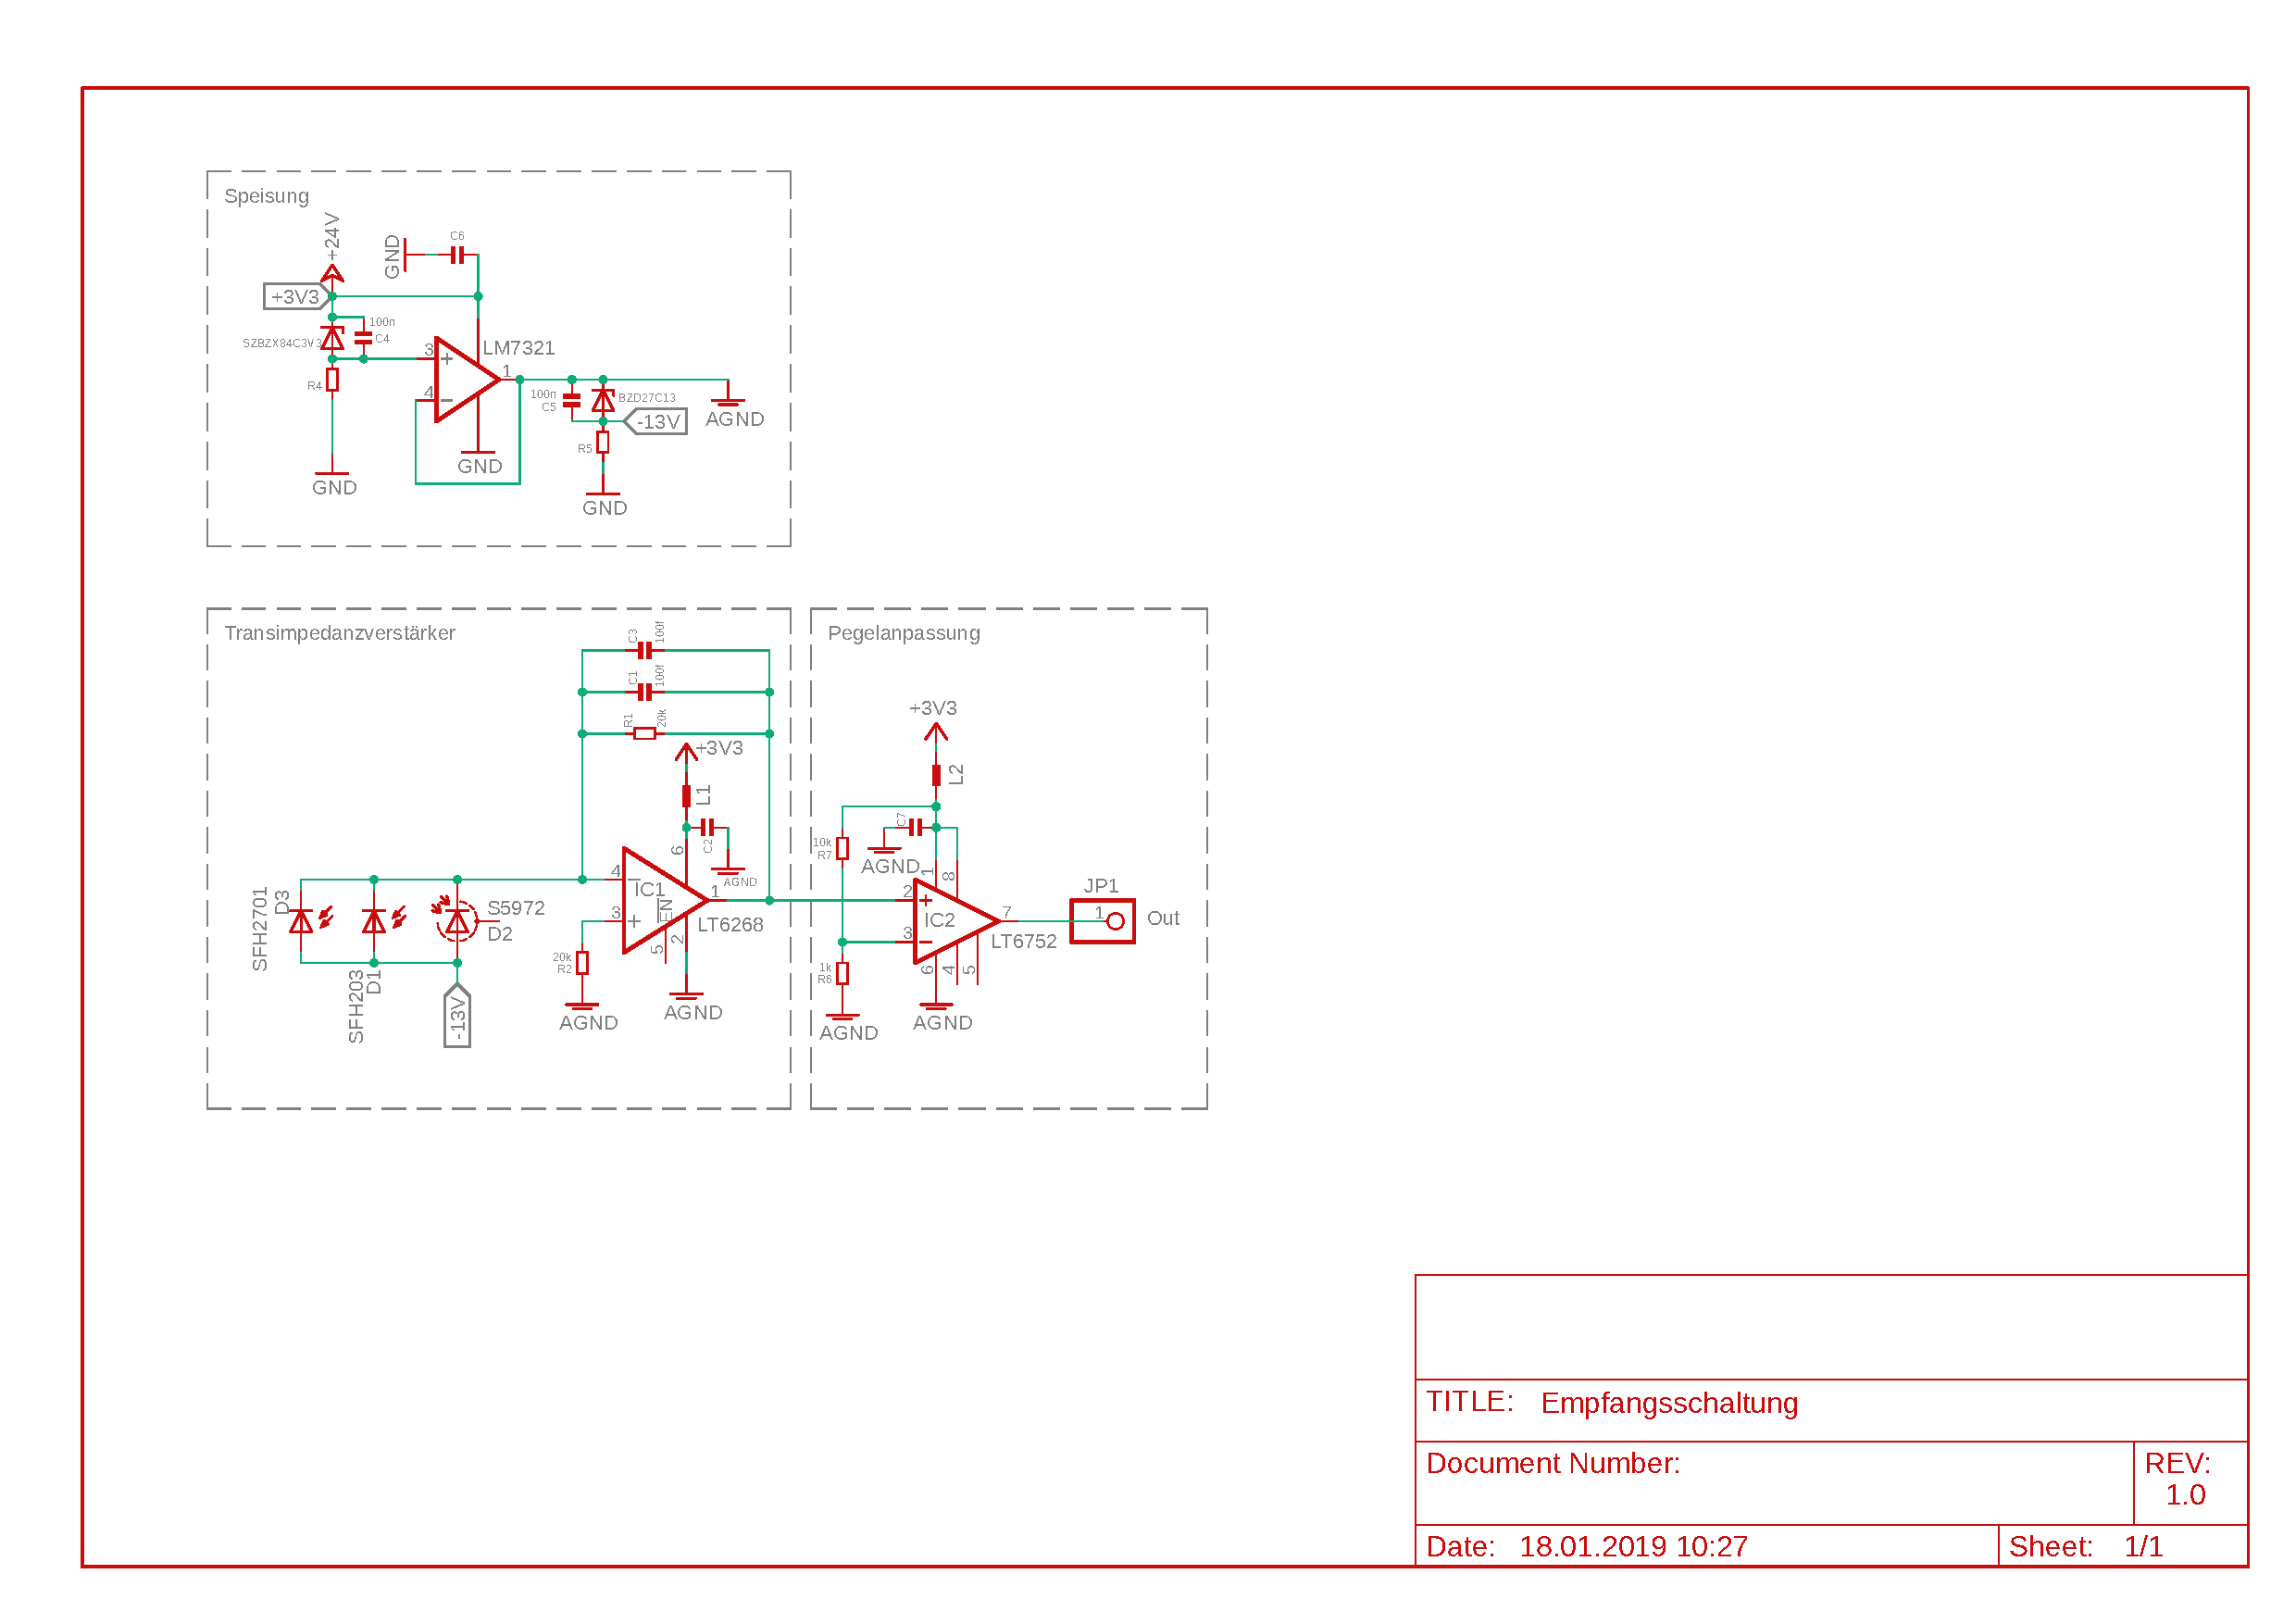
\includepdf[pages={1},fitpaper,nup=1x1,landscape=true,scale=0.85,offset=10 -40,pagecommand={\section{Schema Empfänger}\label{app:Schema_Empfaenger}\thispagestyle{myheadings}}]{appendix/Schema_Empfaenger.pdf} \newpage

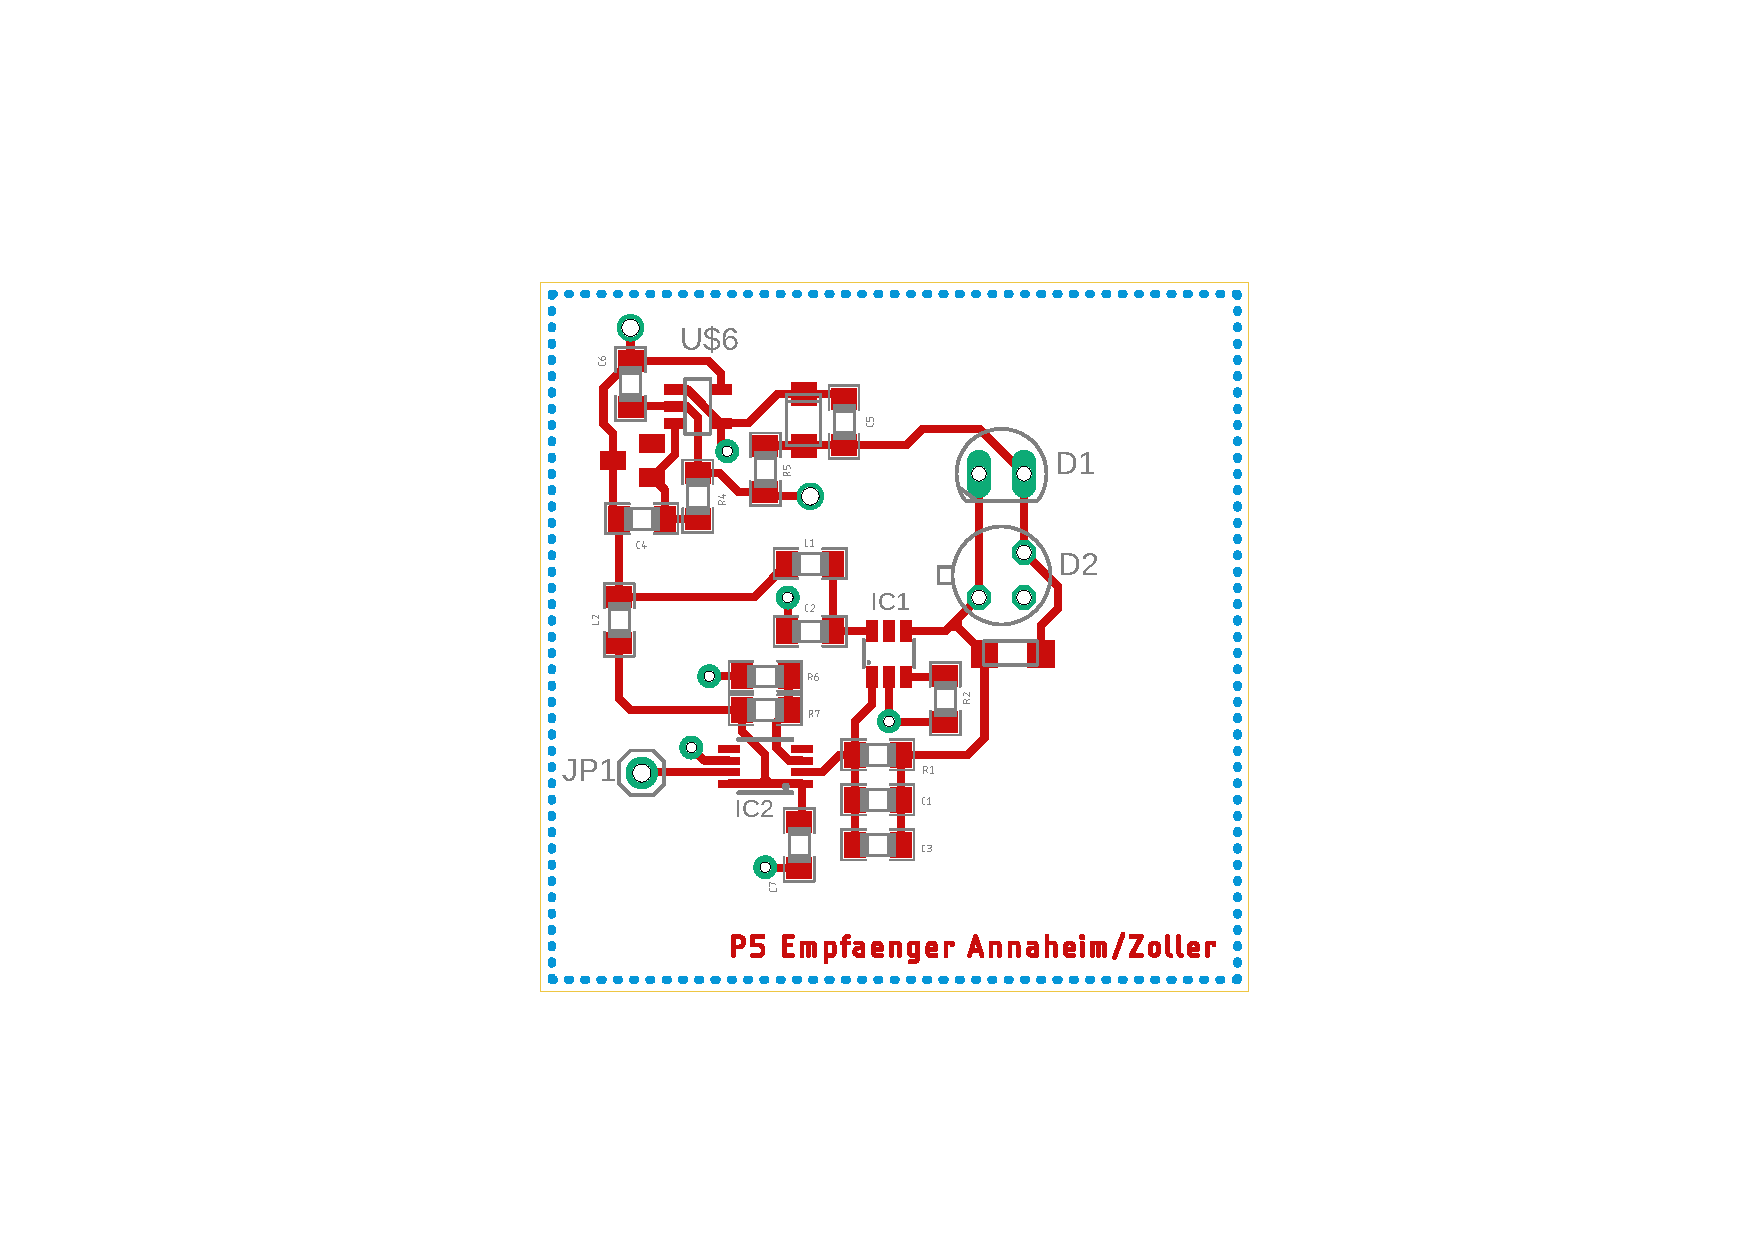
\includepdf[pages={1},nup=1x1,landscape=true,scale=0.85,offset=10 -40,pagecommand={\section{Layout Empfänger}\label{app:Layout_Empfaenger}\thispagestyle{myheadings}}]{appendix/Layout_Empfaenger.pdf} \newpage

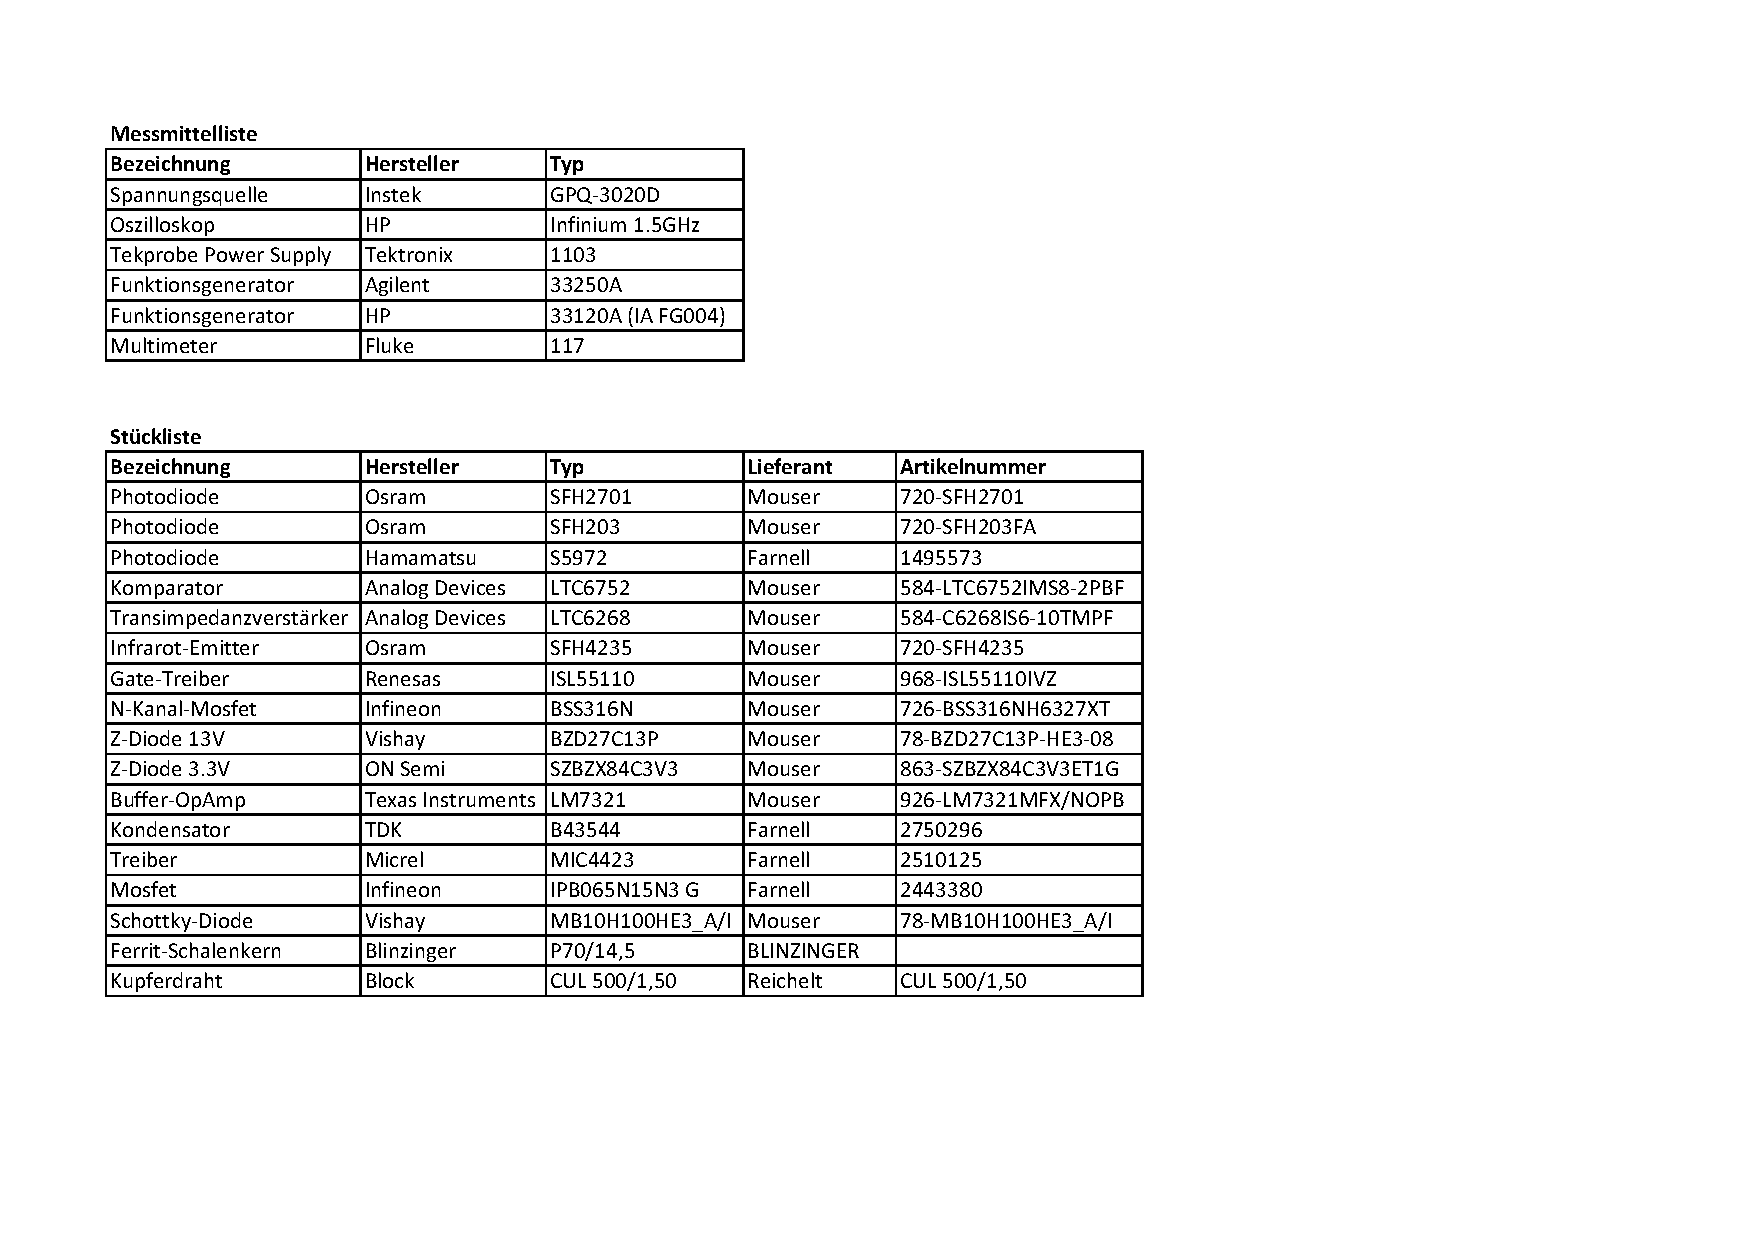
\includepdf[pages={1},nup=1x1,landscape=true,scale=0.85,offset=10 -40,pagecommand={\section{Messmittel- und Stückliste}\label{app:Messmittel}\thispagestyle{myheadings}}]{appendix/Messmittelliste.pdf} \newpage

\end{appendix}


%%---NOTES for DEBUG---------------------------------------------------------------------
\ifdraft{%Do this only if mode=draft
%%requires \usepackage{todonotes})
\newpage
\listoftodos[\section{Todo-Notes}]
\clearpage
}
{%Do this only if mode=final
}
\end{document}
